\subsection{Multijet Background Estimation}
\label{sec:multijet_background}
As discussed above, the SM backgrounds are estimated from Monte-Carlo simulation and constrained in the dedicated control regions. However, the multijet processes is poorly modelled in MC simulation due to the lack of understanding if QCD, so simulation is not feasible for this background contribution. Its contribution is from the following sources:
\begin{itemize}
	\item {\bf Photon Conversion}: When photons or pions interact with the detector material, they decay to soft leptons with similar behaviour to signal ones, which is difficult to recognize. This contribution is mainly into electron, while it could be suppressed by combined muon requirement in muon channel
	\item {\bf Lepton Misidentification}: Soft charged partons could be blocked at ECAL and leave no signature in HCAL, which is identical to electron signatures. In this case, they are reconstructed as electrons instead of jets. This source only contributes to electron channel.
	\item {\bf Heavy Hadron Decay}: The decay products of heavy partons also include leptons. If their decay is close to the primary vertex, the decayed leptons are not distinguishable from the prompt ones. Both electrons and muons have the contribution from this source. 
\end{itemize}
\noindent
As an alternative, the estimation is performed with fake factor method, a data-driven approach. It is only significant in resolved channel while begin negligible in boosted channel.  The details of this method could be found in the ATLAS Run2 VHbb analysis~\cite{ATLAS-CONF-2016-091, ATL-COM-PHYS-2016-429}. 
\\
\\{\bf Methodology}
\\
\\In the method, to be orthogonal to the signal and control region, fake factors are estimated in the region with only one small R jet called single jet control region where the existence of fat jet passing the selection is not allowed ($p_{T}^{J}>200~GeV$ \&\& $m^{J}>50~GeV$) to keep the orthogonality to boosted region. This region is then further divided into two subregions by lepton isolation, as shown in table \ref{tab:LepIsoCR}. With $p_{T}(\mu\nu)<150~GeV$, an isolated muon trigger is applied with isolation, $ptvarcone/p^{\mu}_{T}<0.07$ (at trigger level). In this case, the isolation requirement for inverse muon is tightened to $ptvarcone/p^{\mu}_{T}<0.07$ to keep the consistency of muons reconstructed at trigger and offline stages. As region $p_{T}(\mu\nu)>150 GeV$ is using $E_{T}^{miss}$ trigger, so the isolation bias is not present. Fake factors in the dedicated bins are defined as:
\begin{equation}
 f = \frac{N_{event}(CR(1j, \mu\left[signal\right]))}{N_{event}(CR(1j, \mu\left[inverse\right]))}
\end{equation}
with the binning in Table~\ref{tab:FFBinning}. Fake factors have the dependence on lepton eta (this dependence is for the consideration of detector homogeneity) and $p_{T}$. Additional binning on the $E_{T}^{miss}$ is applied in electron channel. For both channels, the fake factor is estimated in two different regions with $p_{T}(\mu\nu)<150~GeV$ and $p_{T}(\mu\nu)>150~GeV$ to achieve better precision. Fake factor is shown as a function of lepton $p_{T}$ in Figure~\ref{fig:fakefactor} for the region of $p_{T}(l\nu)>150~GeV$. It could be noticed that fake factor for electron channel is just up to $p_{T}=190~GeV$. For better accuracy, the fake factor for high $p_{T}$ electron is roughly evaluated in $p_{T}$ bins only which is shown in Figure~\ref{fig:fakefactor_el_highPt}.

\begin{table}[h]
  \caption{Isolation for leptons in the single jet control region} \label{tab:LepIsoCR}
  \begin{center}

    \begin{tabular}{ | c | c | c | }
     \hline
                               &   SingleJetSigLepCR   & SingleJetInvLepCR \\ \hline
    electron                   &        TightLH        & MediumLH (!TightLH) \\ \hline
    muon($p_{T}(l\nu)>150 GeV$) &  $Iso_{trk}<0.06$    & $0.06<Iso_{trk}<0.15$ \\ \hline
    muon($p_{T}(l\nu)<150 GeV$) &  $Iso_{trk}<0.06$    & $0.06<Iso_{trk}<0.07$ \\ \hline
\end{tabular}
\end{center}
\end{table}


\begin{table}[h]
  \caption{Binning for electrons and muons to evaluate fake factor} \label{tab:FFBinning}
\begin{center}

\begin{tabular}{ | c | c | c | c |}
    \hline
    channel  & $p_{T}(GeV)$ & $|\eta|$ & $E_{T}^{miss}(GeV)$ \\ \hline
    electron & 27-115 &  & 0, 60, 75, $\infty$ \\
             & 115-135&0, 1.37, 1.52, 2.47 & 0, 38, 52, $\infty$ \\
             & 135-155& & 0, 26, 43, $\infty$ \\
             & 155-190& & 0, 25, 45, $\infty$ \\ \hline
    muon     & 27, 42, 59, 76, 99, $\infty$ & 0, 1.05, 1.5, 2.5 & N/A \\ \hline

\end{tabular}
\end{center}
\end{table}

\begin{figure}[ht]
       \centering
       \subfloat[]{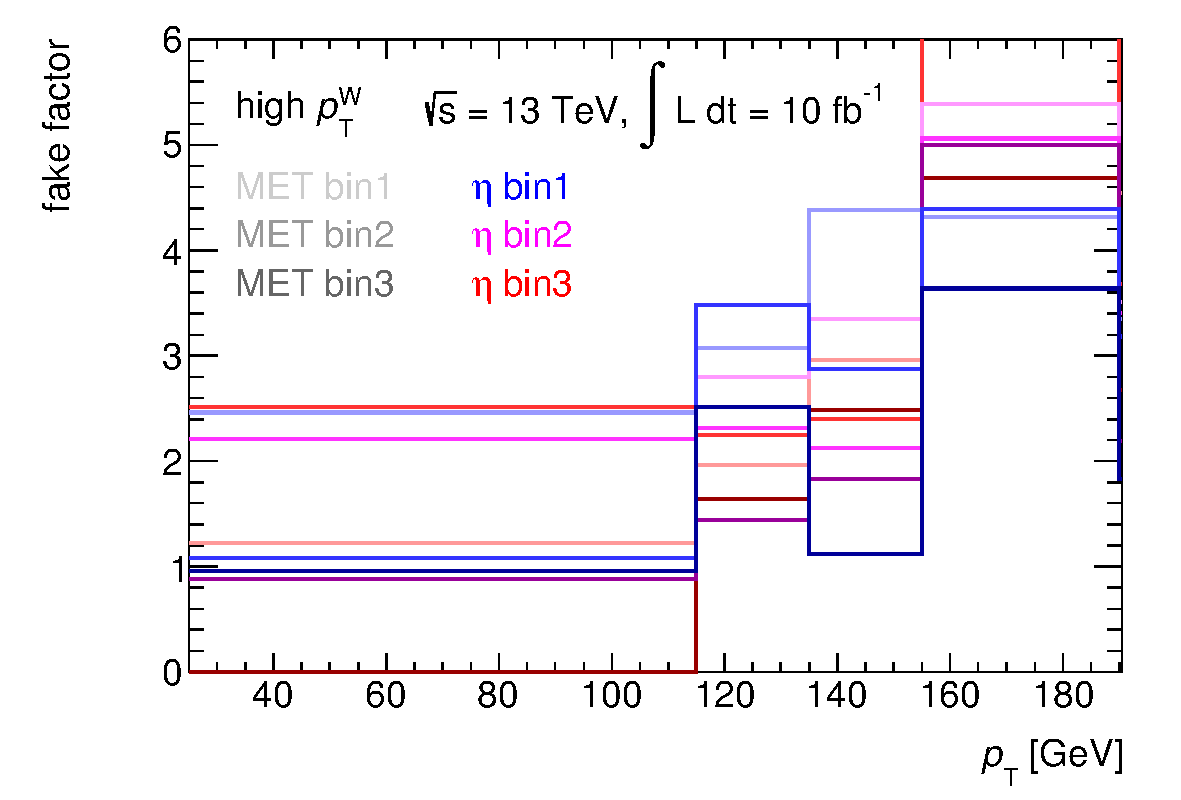
\includegraphics[width=0.4\textwidth]{Chapter3/fakefactor_el_medium_highpTW}}
       \subfloat[]{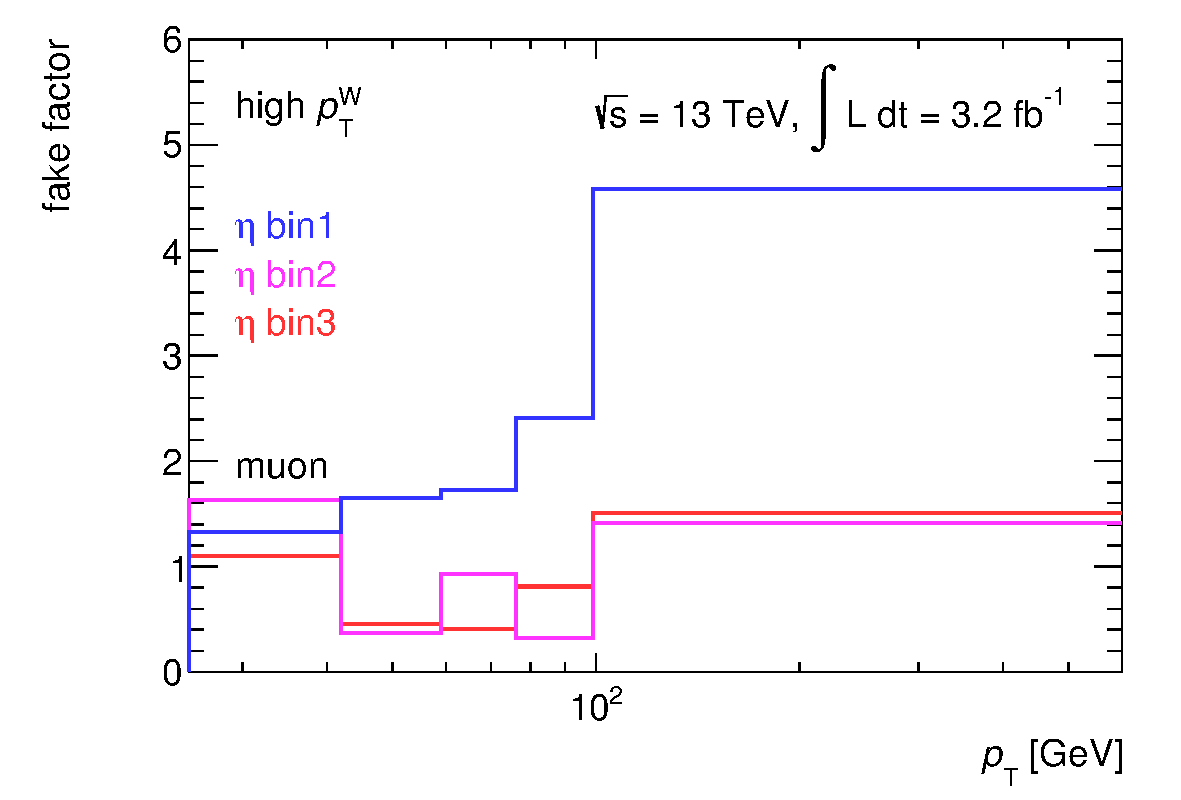
\includegraphics[width=0.4\textwidth]{Chapter3/fakerate_mu_ewk}} \\
       \caption{Fake factors for the corresponding binnings (shown in text) in electron (a) and muon (b) channels}
       \label{fig:fakefactor}
\end{figure}

\begin{figure}[ht]
       \centering
       \subfloat[]{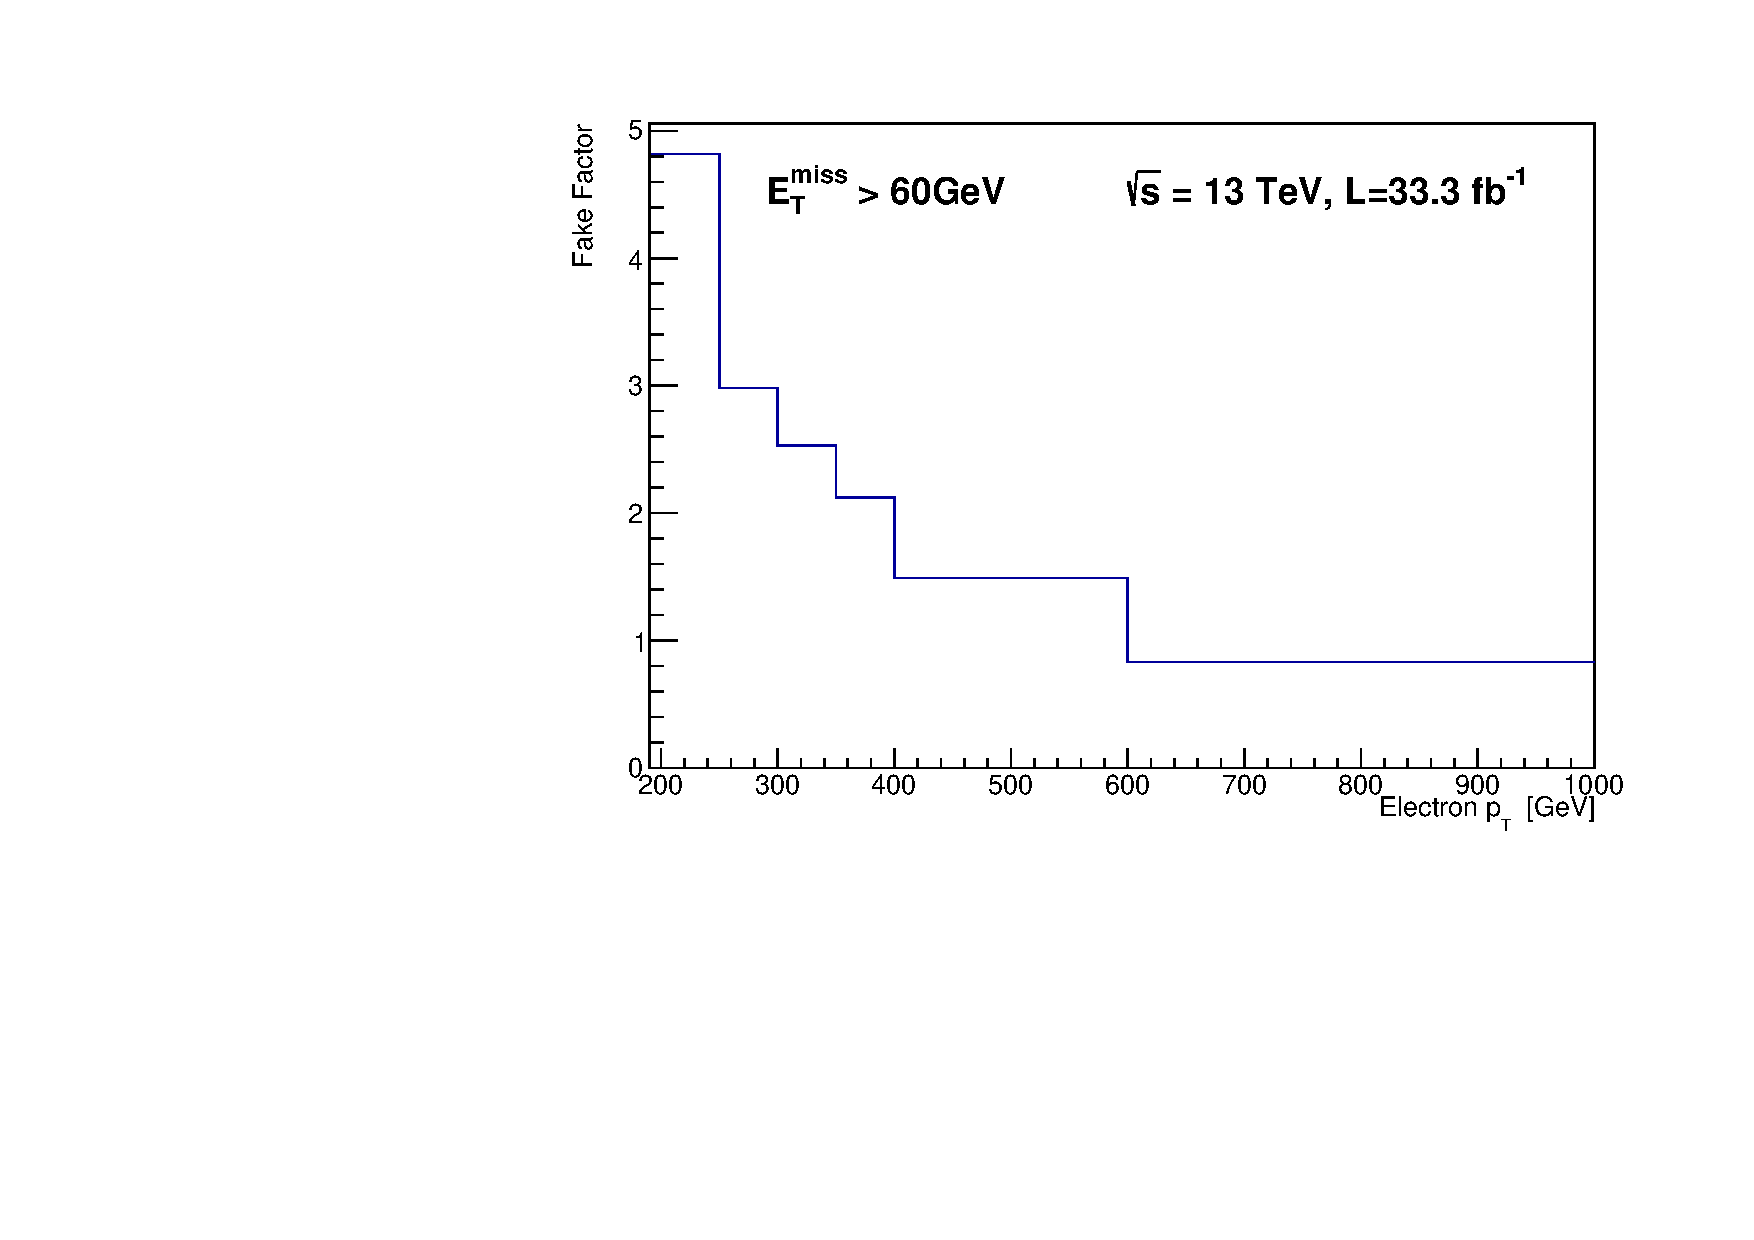
\includegraphics[width=0.4\textwidth]{Chapter3/fakerate_el_highPt.pdf}}
       \caption{Fake factors for high $p_T$ electrons}
       \label{fig:fakefactor_el_highPt}
\end{figure}


\subsubsection*{Electroweak Subtraction}

Electroweak interactions ($t\bar{t}$, W/Z+jets, diboson and single top) could also contribute to multijet events in addition to the multijet background, so they might be double counted from fake factor estimation and Monte Carlo simulation. To avoid this issue, those events are removed by employing fake factor estimation on Monte Carlo samples, which could be expressed as the following equation:
\begin{equation}
 N^{MJ}_{events} = N^{data}_{events}-N^{MC}_{event}
\end{equation}
and it is anticipated that $N^{data}_{events}\approx N^{MC}_{event}$ with $E^{miss}_{T}>150GeV$. A control region was defined to verify this with a simple selection of at least two jets with $P_{T}>20GeV$ and exactly one signal electron or muon. The comparison between data and the SM background from the MC simulation in this control region is shown in Figure~\ref{fig:dijetFakeCR_el} and Figure~\ref{fig:dijetFakeCR_mu} for electron and muon channels respectively. The observed discrepancy was contributed by the multijet events. However, unfortunately, the inconsistency remains with $E_{T}^{miss}>150 GeV$. That means the multijet events from the SM backgrounds (electroweak interactions) are not well-modelled. In this case, the electroweak subtraction is applied with a scale factor derive from the ratio of events from data and simulation in the bin of $150 GeV<E^{miss}_{T}<250GeV$ defined as: 
\begin{equation}
f = \frac{N_{event}(data)}{N_{event}(MC)}
\end{equation}
It is applied as an additional correction on fake factor for events with $E_{T}^{miss}>150 GeV$ from simulation. The electroweak subtraction factors for electron and muon channels are shown in Table~\ref{tab:ewsubtraction}.

\begin{figure}[ht]
       \centering
       \subfloat[]{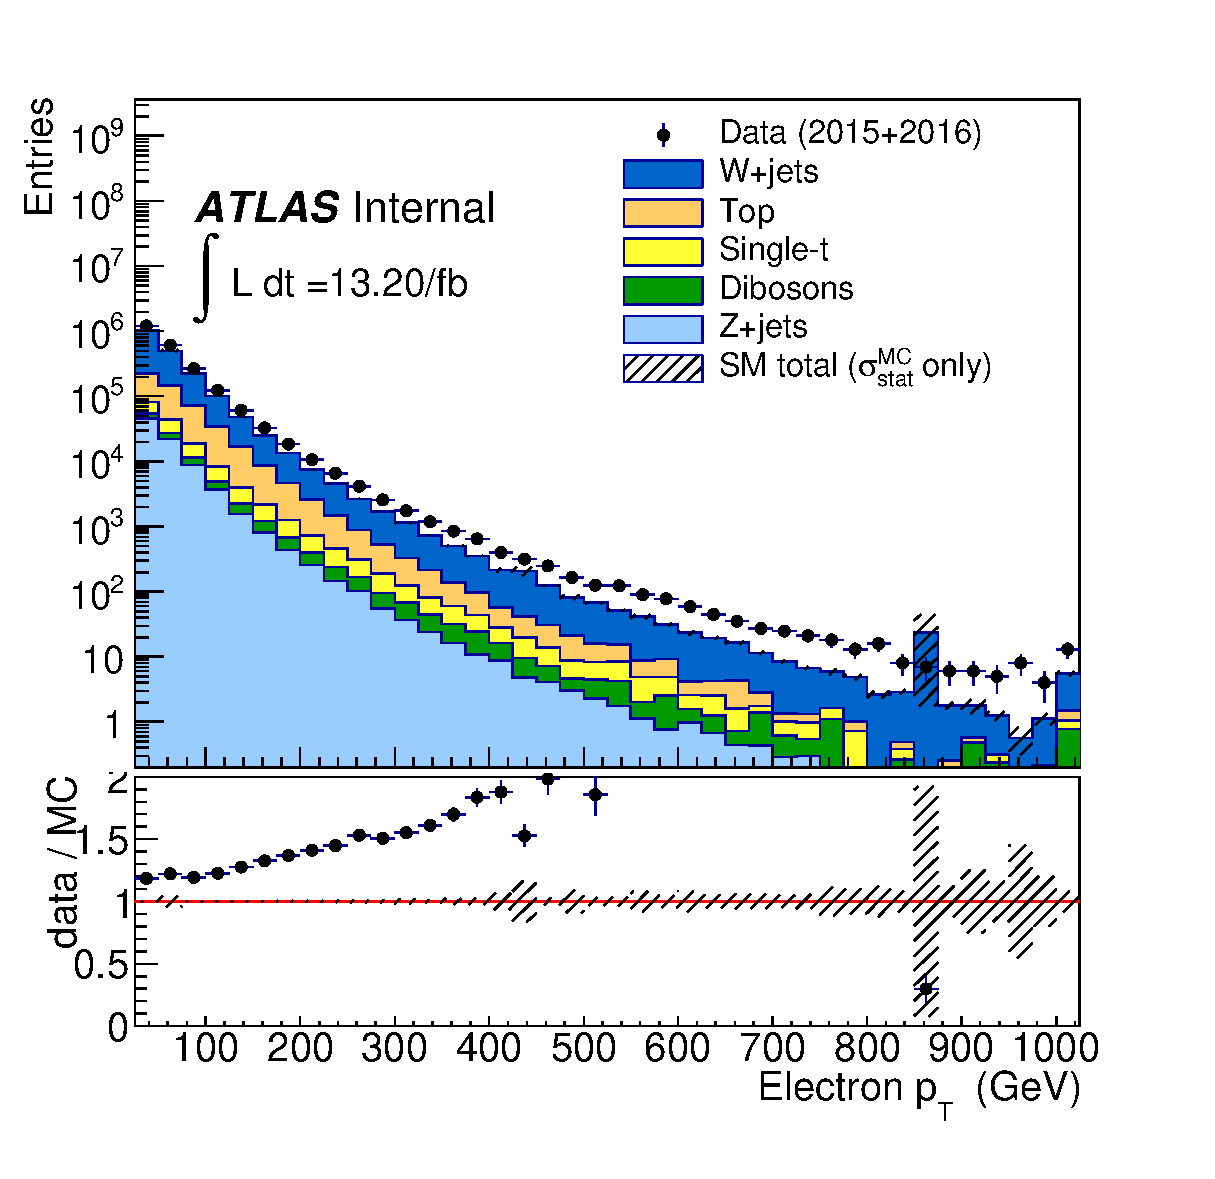
\includegraphics[width=0.45\textwidth]{Chapter3/MJ_CR/electronPt.eps}}
       \subfloat[]{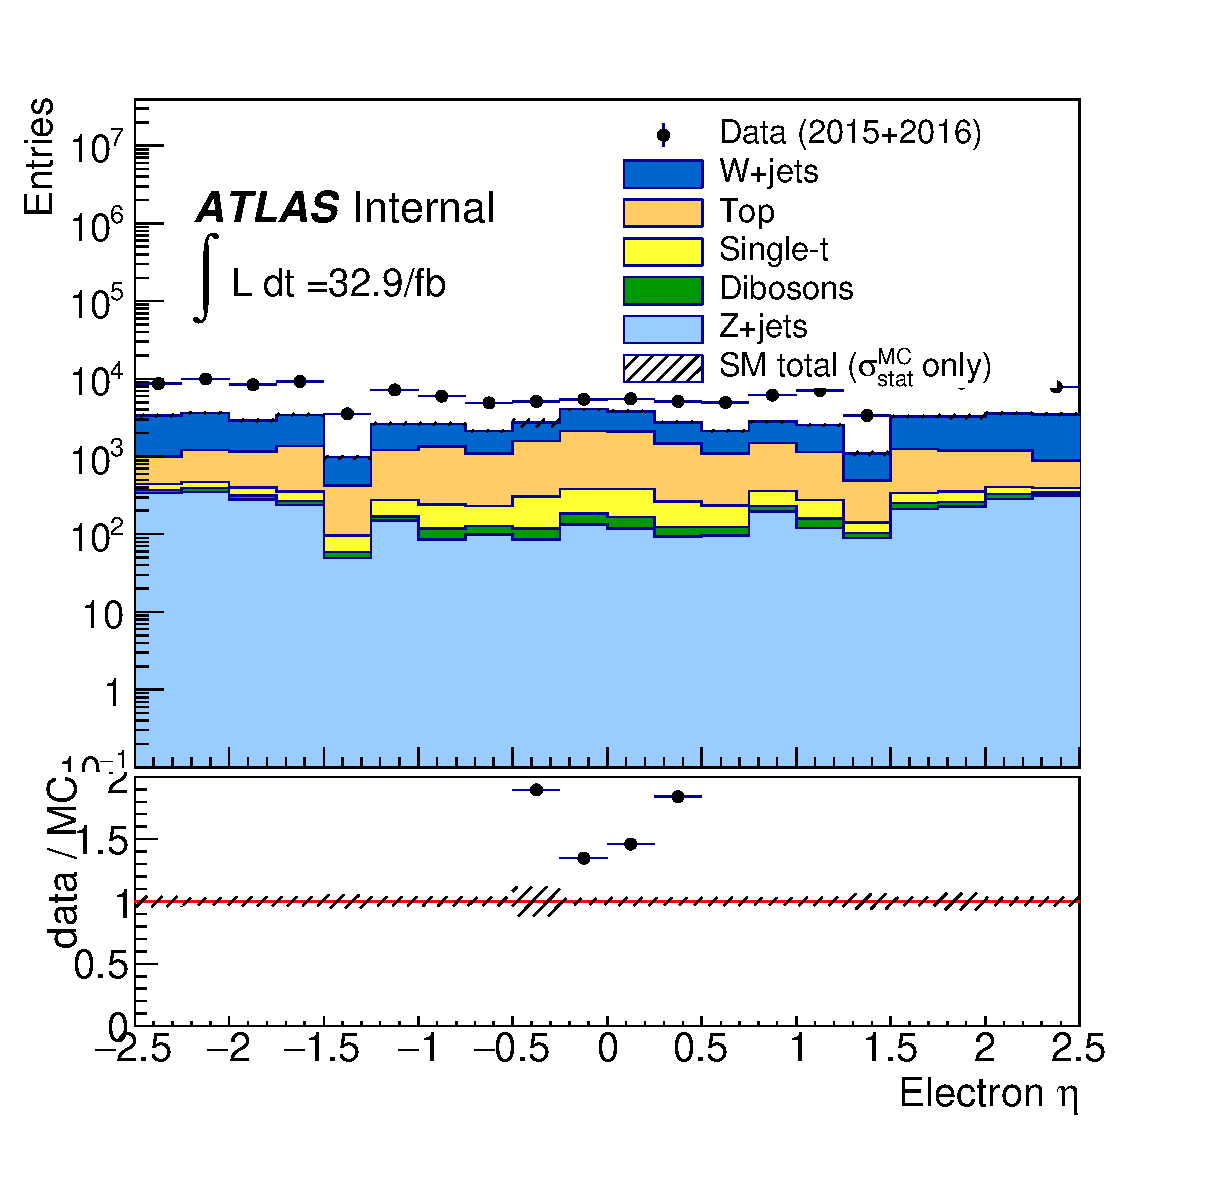
\includegraphics[width=0.45\textwidth]{Chapter3/MJ_CR/electronEta.eps}}\\ 
       \subfloat[]{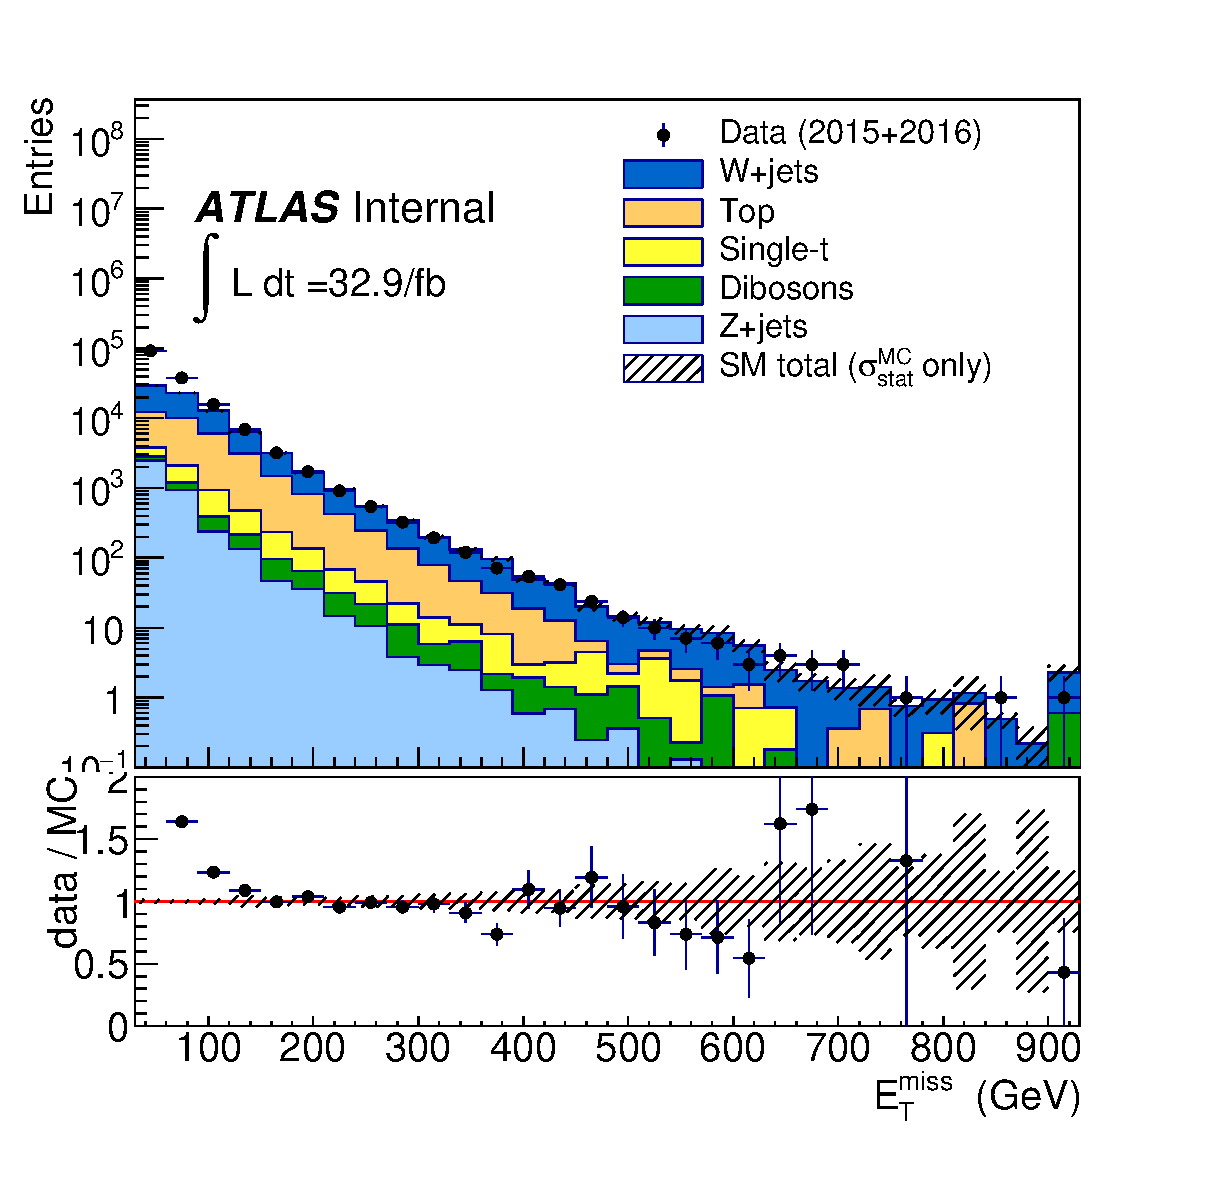
\includegraphics[width=0.45\textwidth]{Chapter3/MJ_CR/met_el.eps}}
       \subfloat[]{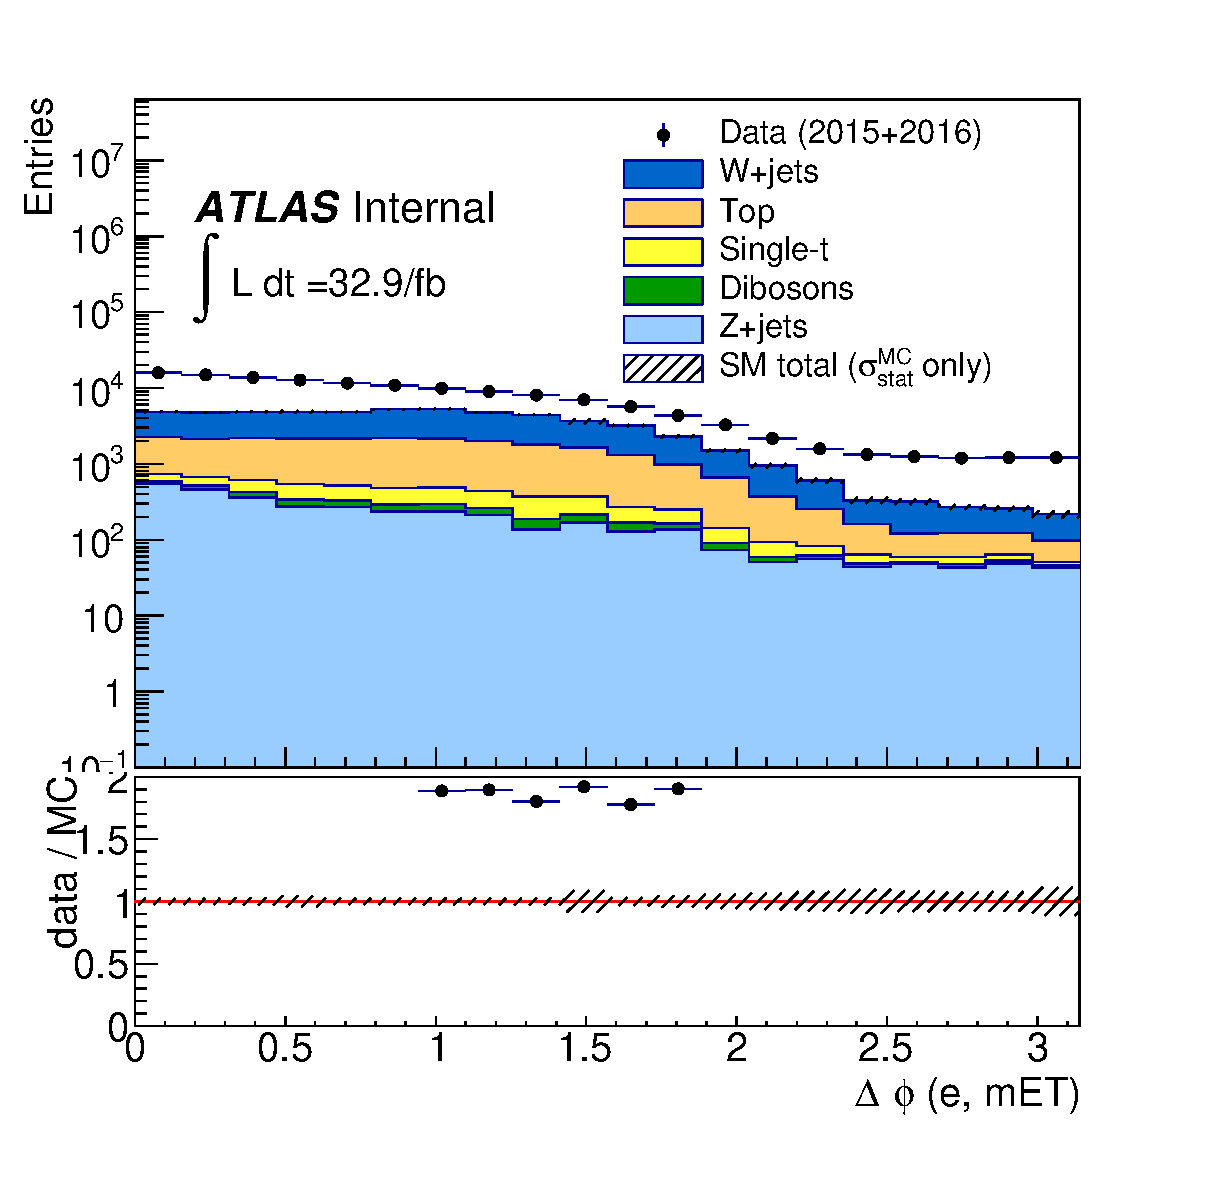
\includegraphics[width=0.45\textwidth]{Chapter3/MJ_CR/dphilepmet_el.eps}}\\
       \caption{The distribution of lepton $p_{T}$,$\eta$, $E_{T}^{miss}$ and $\Delta\phi$(e,$E_{T}^{miss}$) in dijet fake control region with inversed lepton for electron channel. The inconsistency is thought to be comprised of multijet events without applying electroweak subtraction.} 
       \label{fig:dijetFakeCR_el}
\end{figure}

\begin{figure}[ht]
       \centering
       \subfloat[]{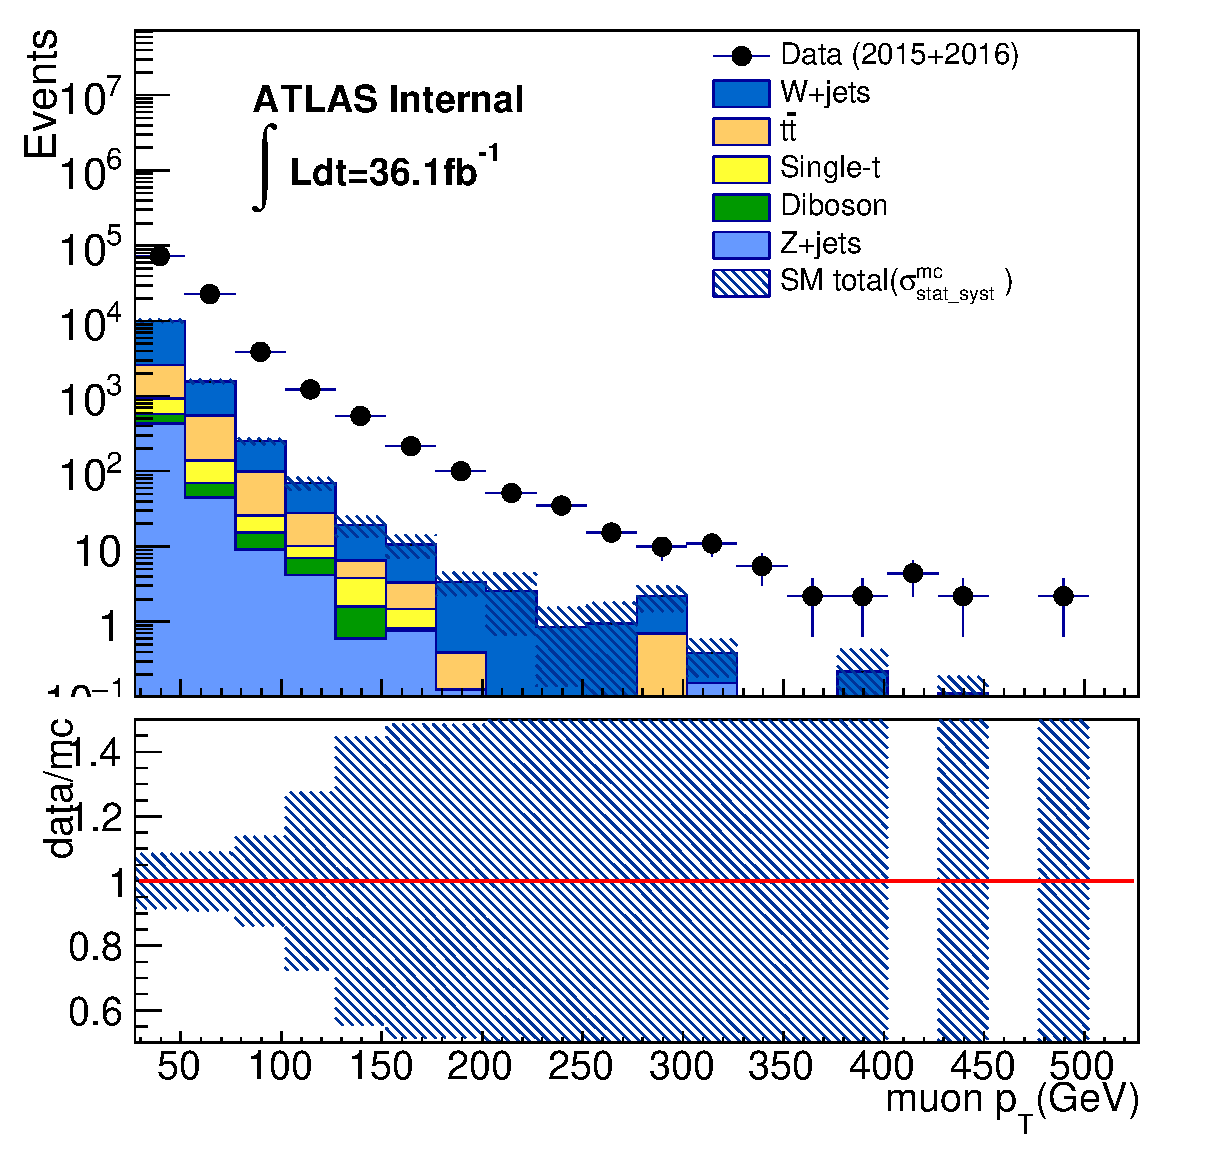
\includegraphics[width=0.45\textwidth]{Chapter3/MJ_CR/muonPt.eps}}
       \subfloat[]{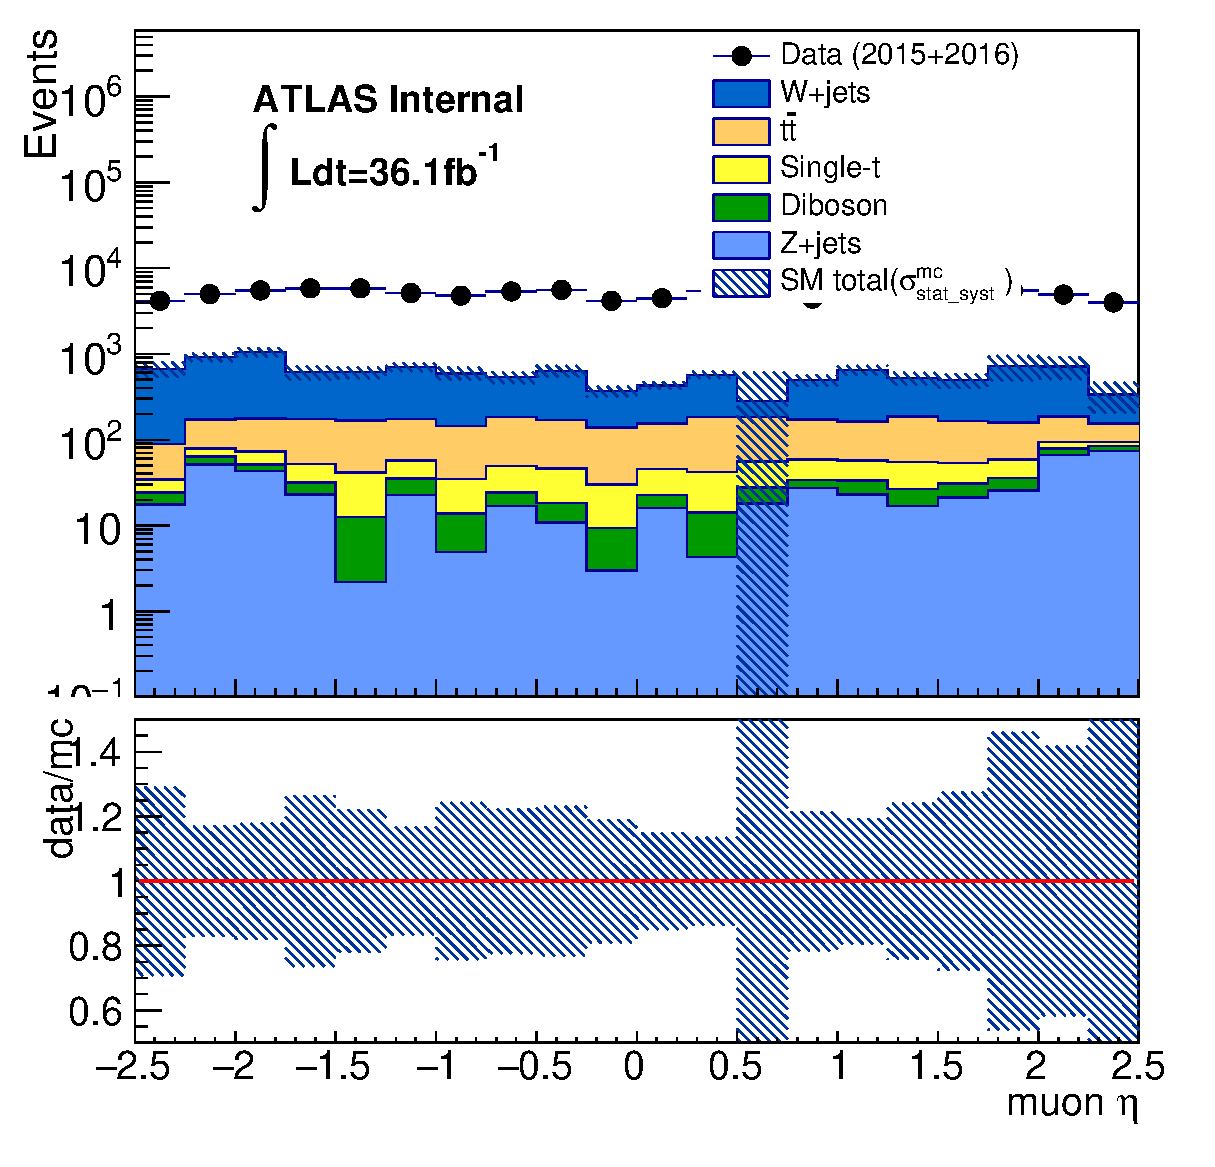
\includegraphics[width=0.45\textwidth]{Chapter3/MJ_CR/muonEta.eps}} \\
       \subfloat[]{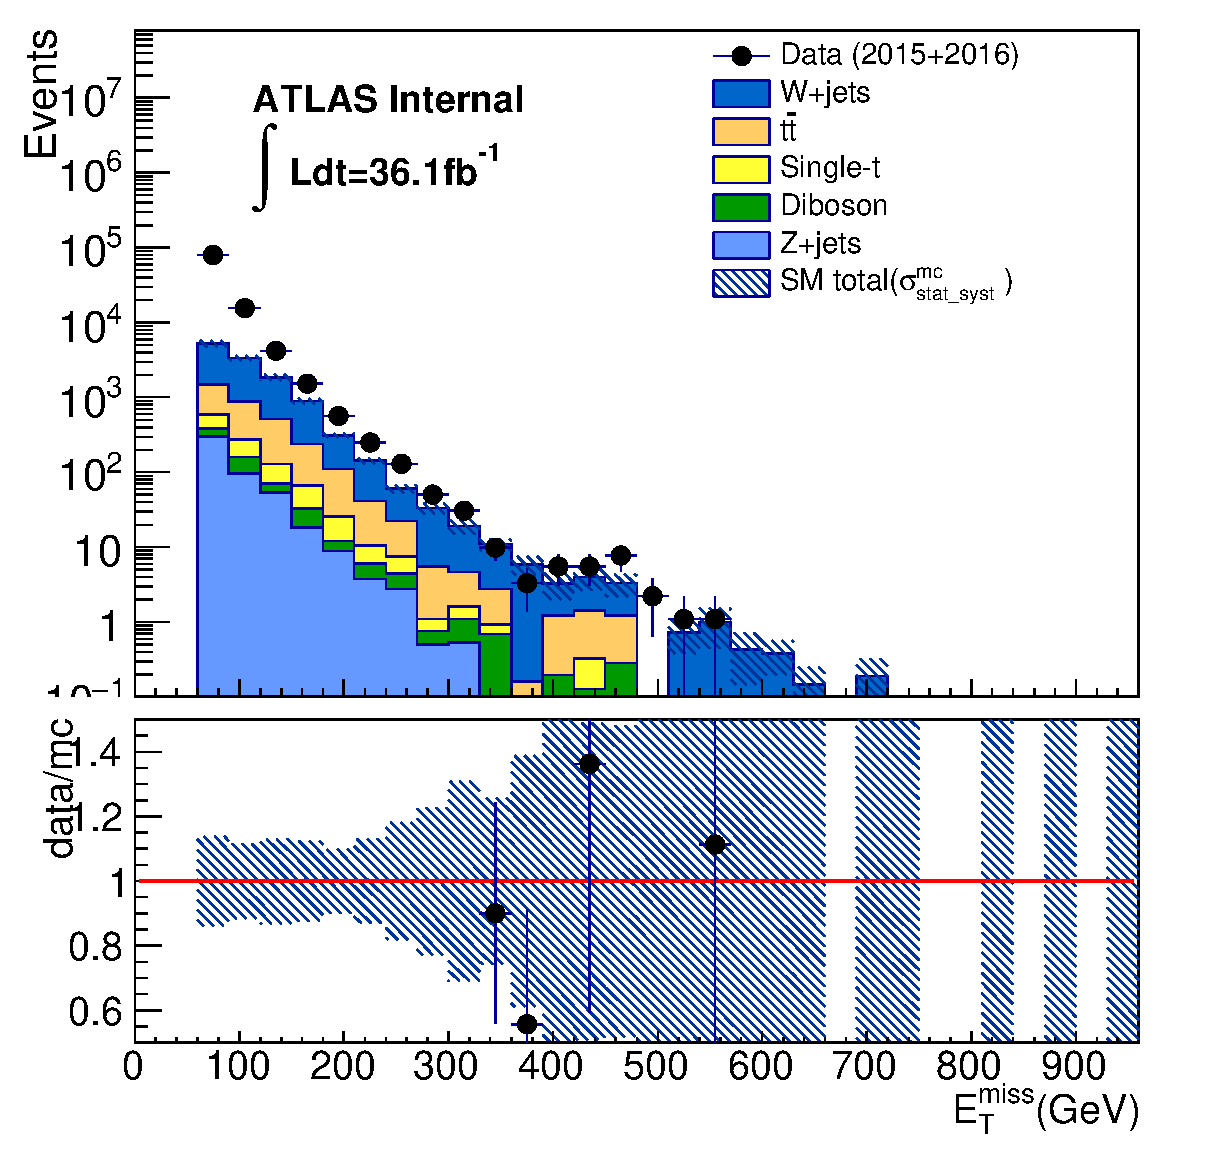
\includegraphics[width=0.45\textwidth]{Chapter3/MJ_CR/met_mu.eps}}
       \subfloat[]{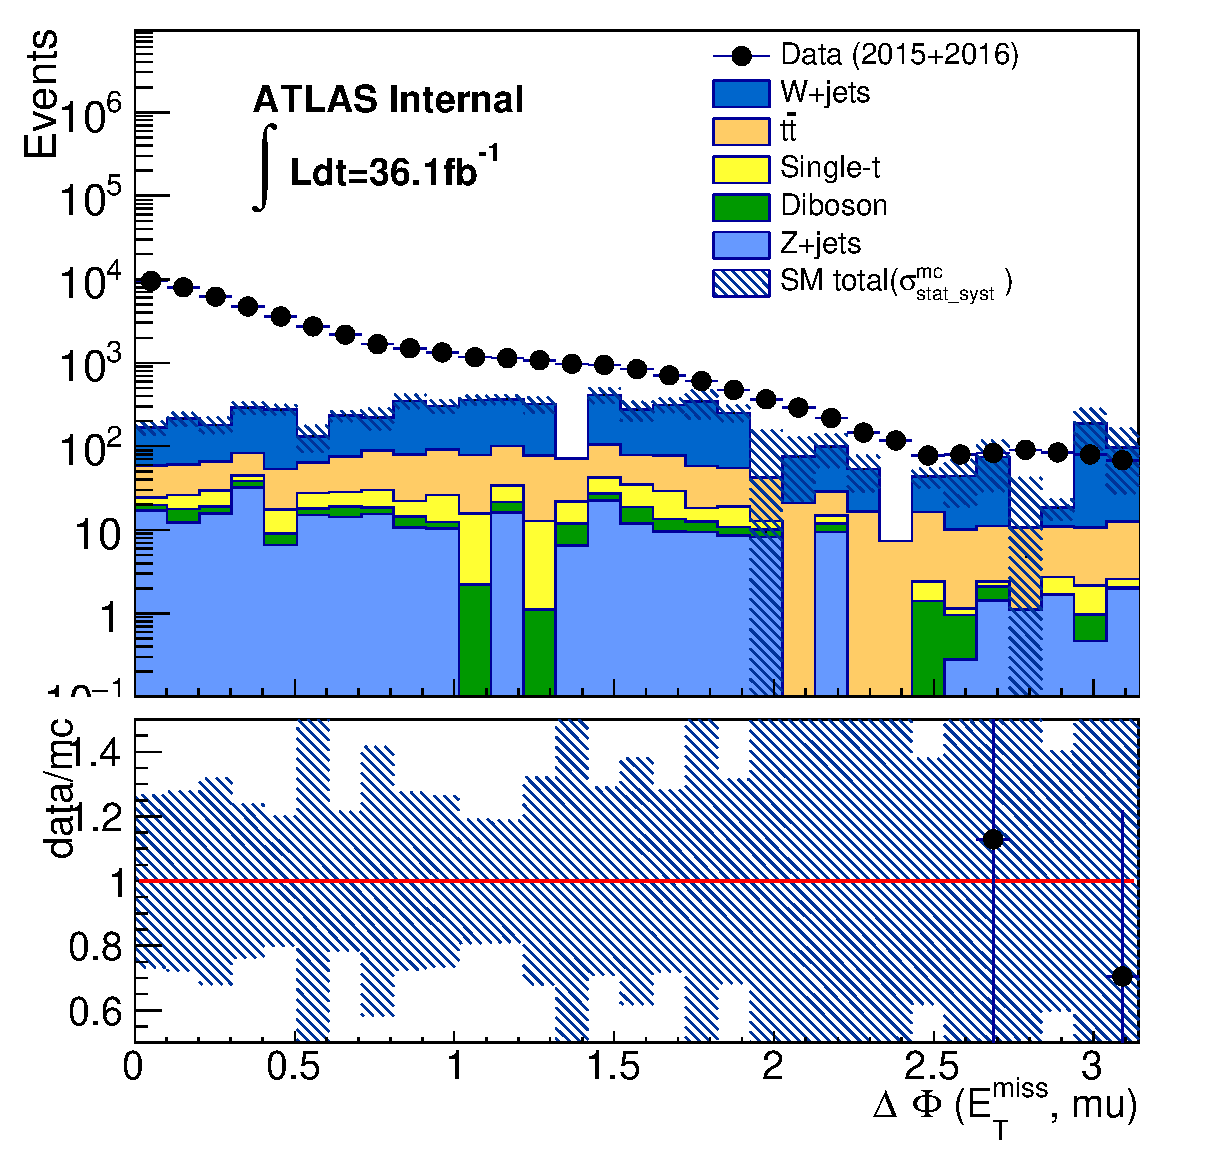
\includegraphics[width=0.45\textwidth]{Chapter3/MJ_CR/dphilepmet_mu.eps}}\\
       \caption{The distribution of lepton $p_{T}$,$\eta$, $E_{T}^{miss}$ and $\Delta\phi$($\mu$,$E_{T}^{miss}$) in dijet fake control region with inversed lepton for muon channel. The inconsistency is thought to be comprised of multijet events without applying electroweak subtraction.}
       \label{fig:dijetFakeCR_mu}
\end{figure}

\begin{table}[h]
  \caption{Electroweak subtraction factor for electron and muon channels} \label{tab:ewsubtraction}
  \begin{center}

    \begin{tabular}{ | c | c | c | }
     \hline
     channels                       &   electron   & muon \\ \hline
     EW subtraction factor          &   1.36       & 1.49 \\ \hline
\end{tabular}
\end{center}
\end{table}

\subsubsection*{Validation}
The method is validated in the dedicated validation region. The definition is similar to the signal region with looser cut to enrich the multijet events. It requires at lease two resolved jets ($p_{T}^{leading}>60GeV$, $p_{T}^{subleading}>45GeV$), $30GeV<E^{miss}_{T}<50GeV$, exactly one isolated lepton and the resolved triggers passed for electron and muon channels respectively. This definition is slightly overlapped with signal and control regions, but the upper cut on $E^{miss}_{T}$ suppress the signal contribution.  As the fake factors were derived from two bins of $p_{T}(l\nu)$, the validation is performed on $p_{T}(l\nu)<150 GeV$ and $p_{T}(l\nu)>150 GeV$. The results are presented in Figures~\ref{fig:FakeVR1_el} -~\ref{fig:FakeVR2_mu} with multijet background estimated using fake factor method. In general, data agrees well with backgrounds with tolerable inconsistency within statistic uncertainties. The disagreement in the region of $p_{T}(l\nu)>150 GeV$ is supposed to be due to the low statistics for fake factor estimation in single jet control region, but it should not have great impact in final interpretation, as multijet events would just account for around 10\% of the whole background. The related systematic uncertainty would be discussed in Chapter~\ref{Ch:resonance_stat}.
\clearpage
\begin{figure}[ht]
	\centering
	\subfloat[]{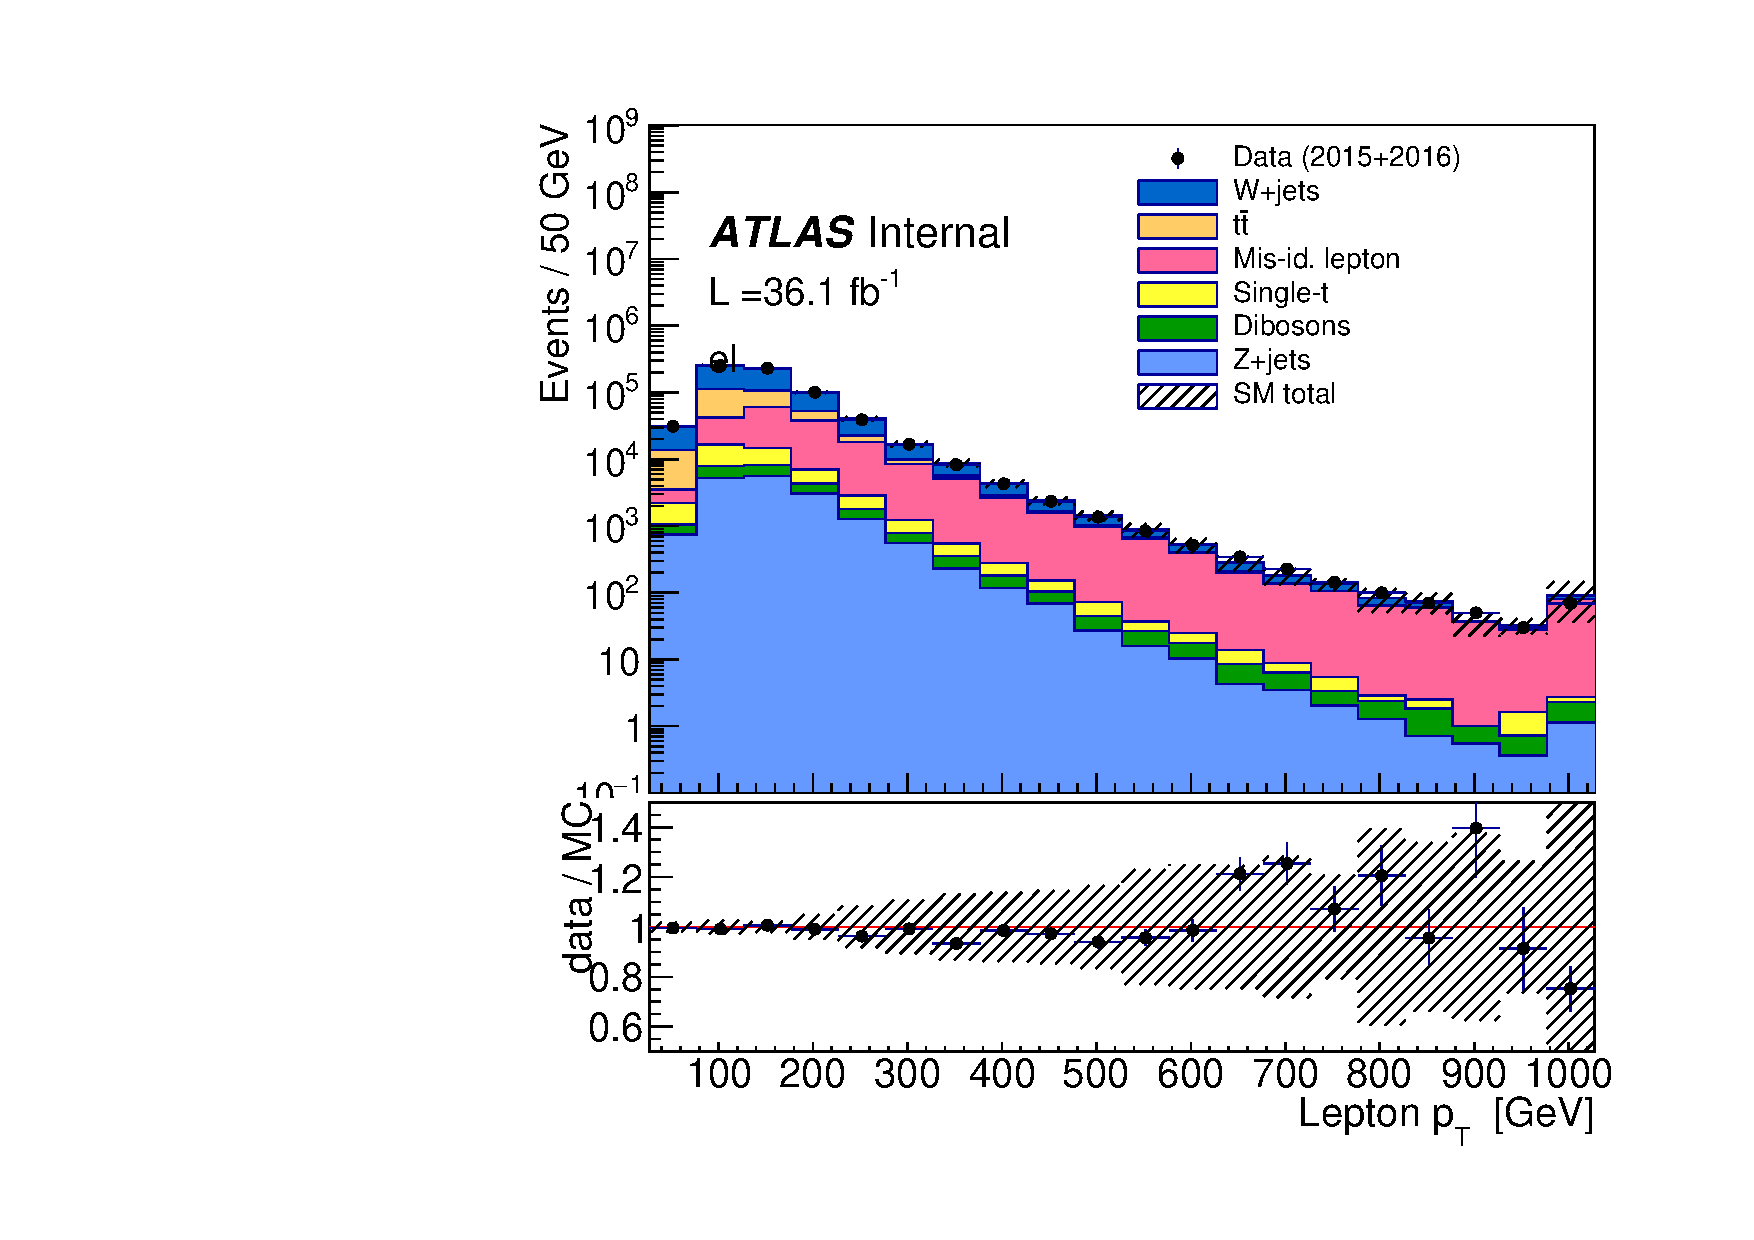
\includegraphics[width=0.43\textwidth]{Chapter3/MJ_VR/lep1pt_Loose_el_highWpt}}
	\subfloat[]{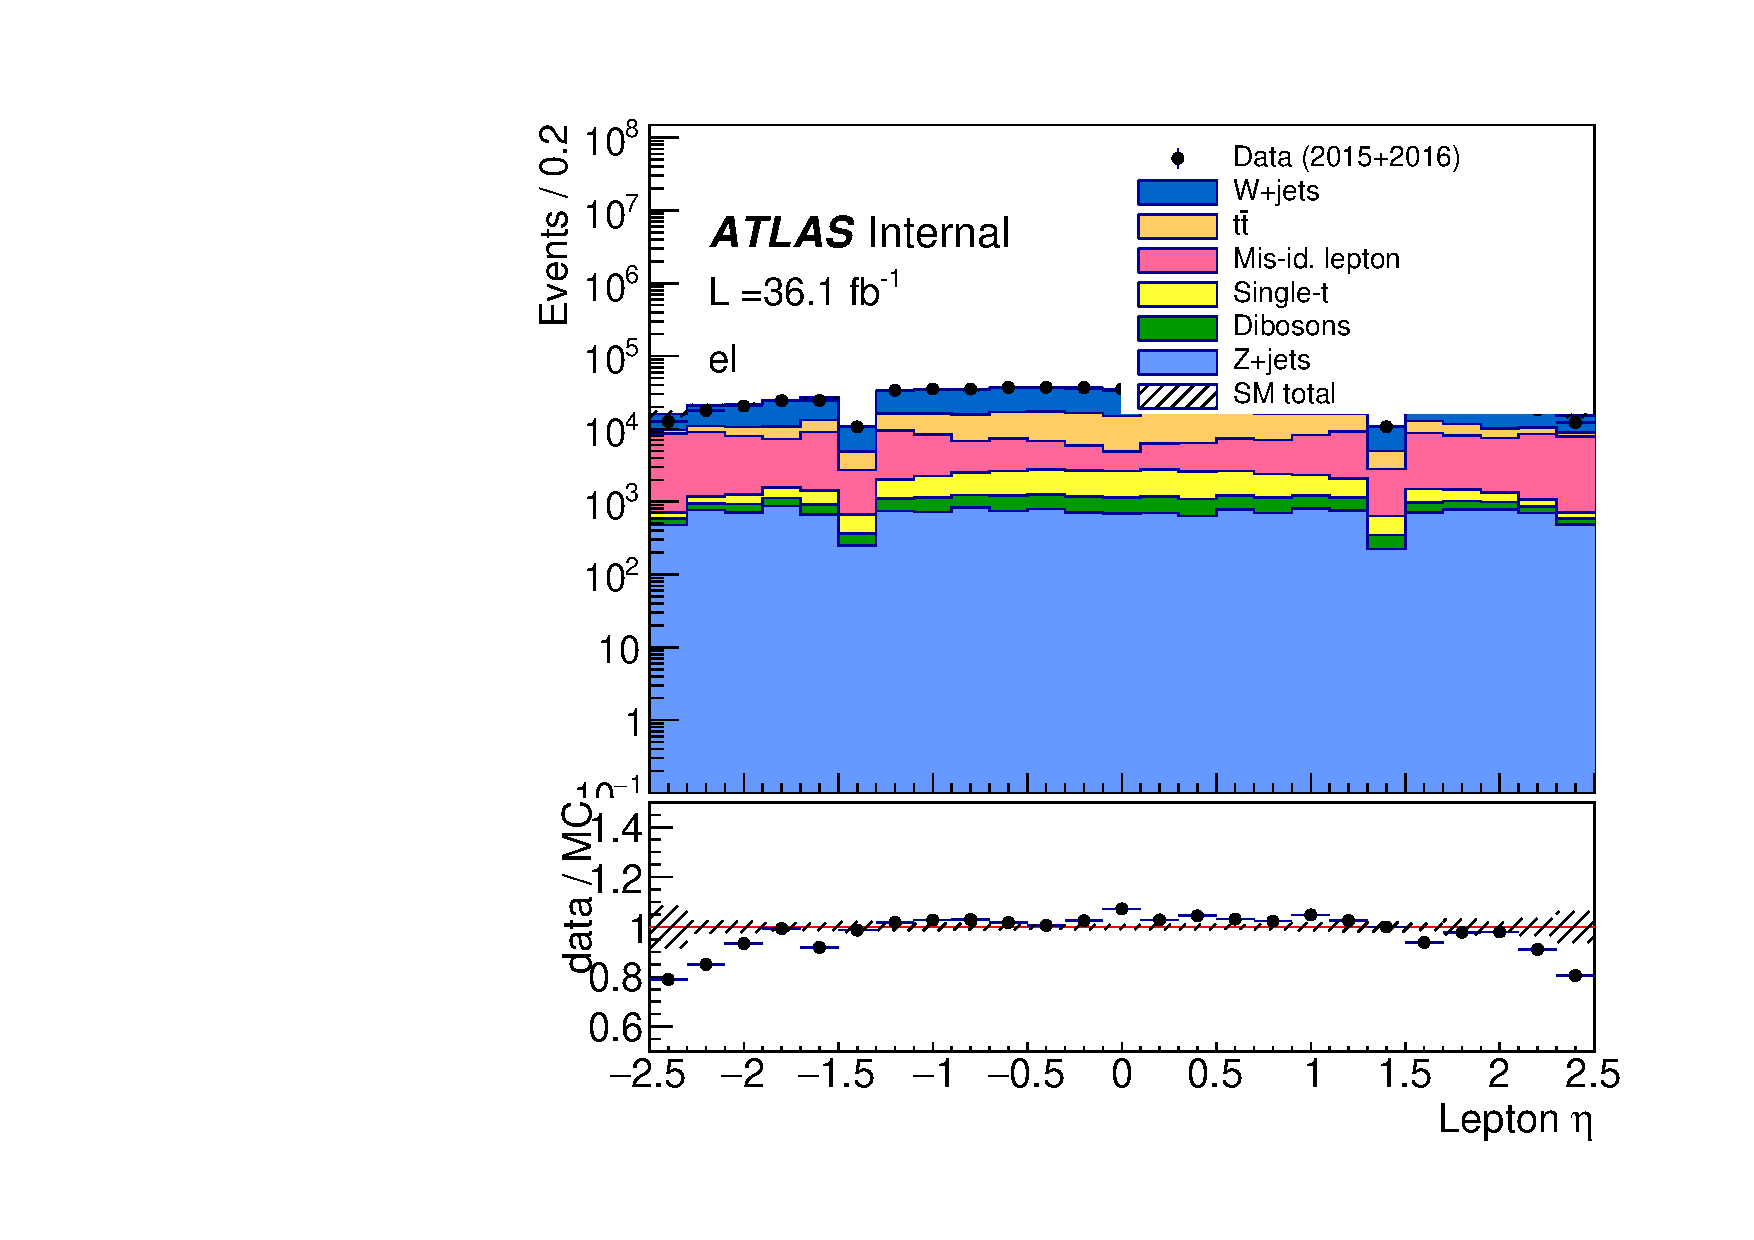
\includegraphics[width=0.43\textwidth]{Chapter3/MJ_VR/lep1eta_Loose_el_highWpt}}\\
	\subfloat[]{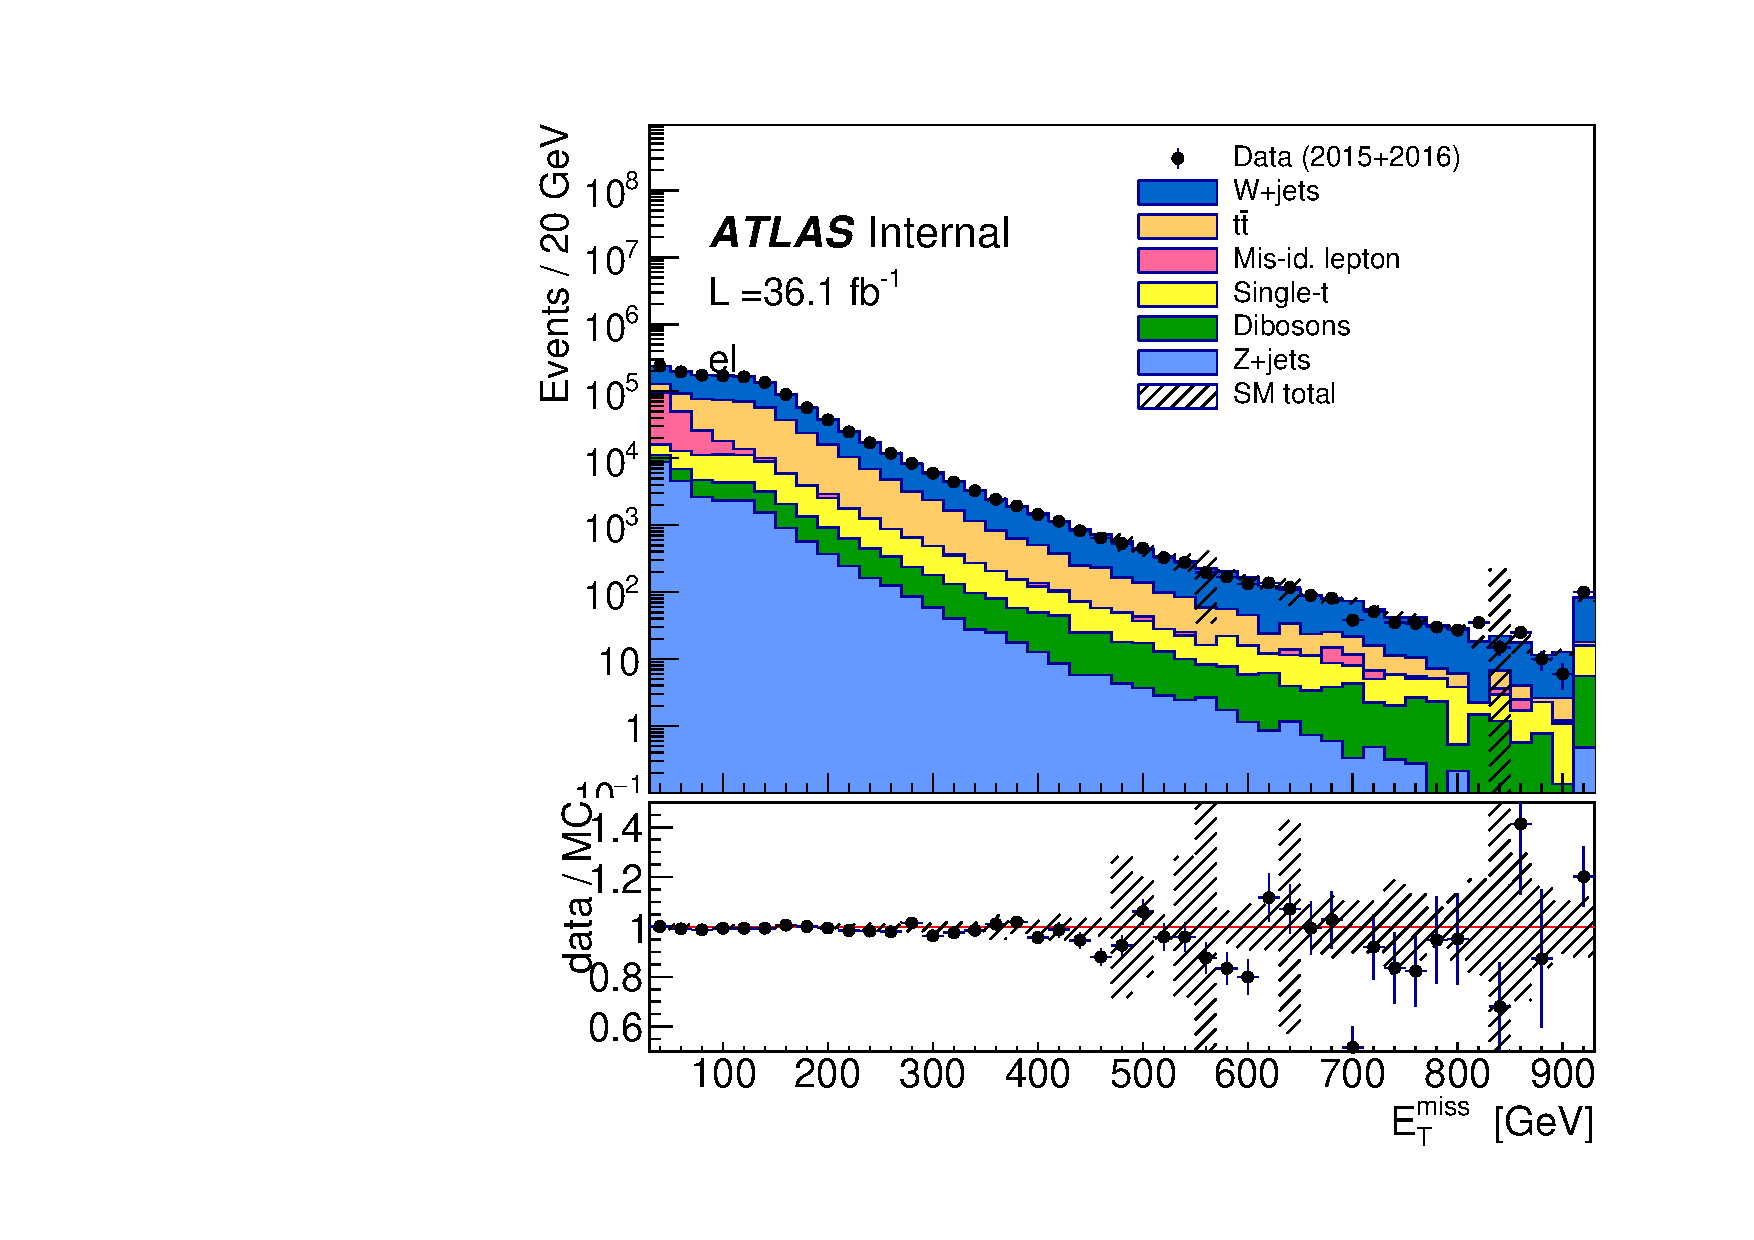
\includegraphics[width=0.43\textwidth]{Chapter3/MJ_VR/met_Loose_el_highWpt}}
	\subfloat[]{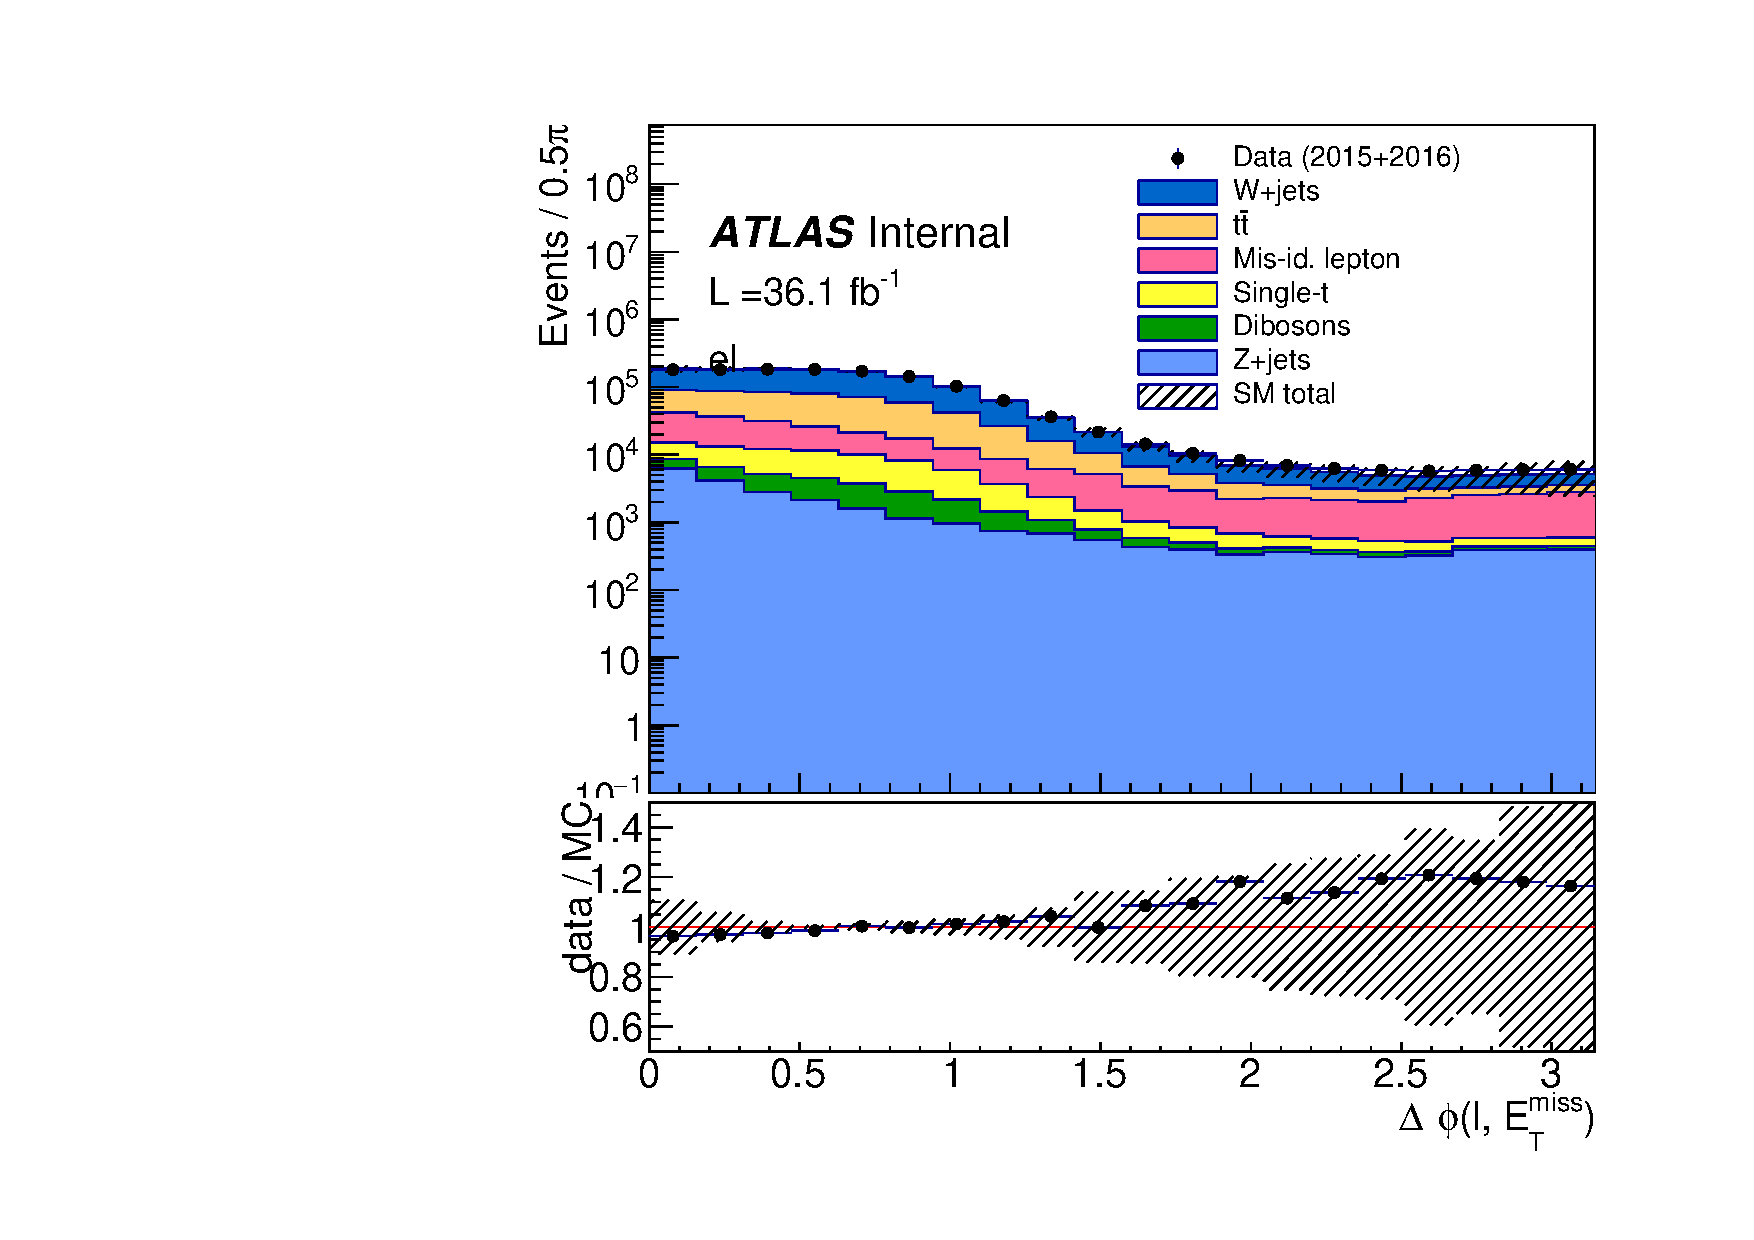
\includegraphics[width=0.43\textwidth]{Chapter3/MJ_VR/dphilepmet_Loose_el_highWpt}}\\
	\subfloat[]{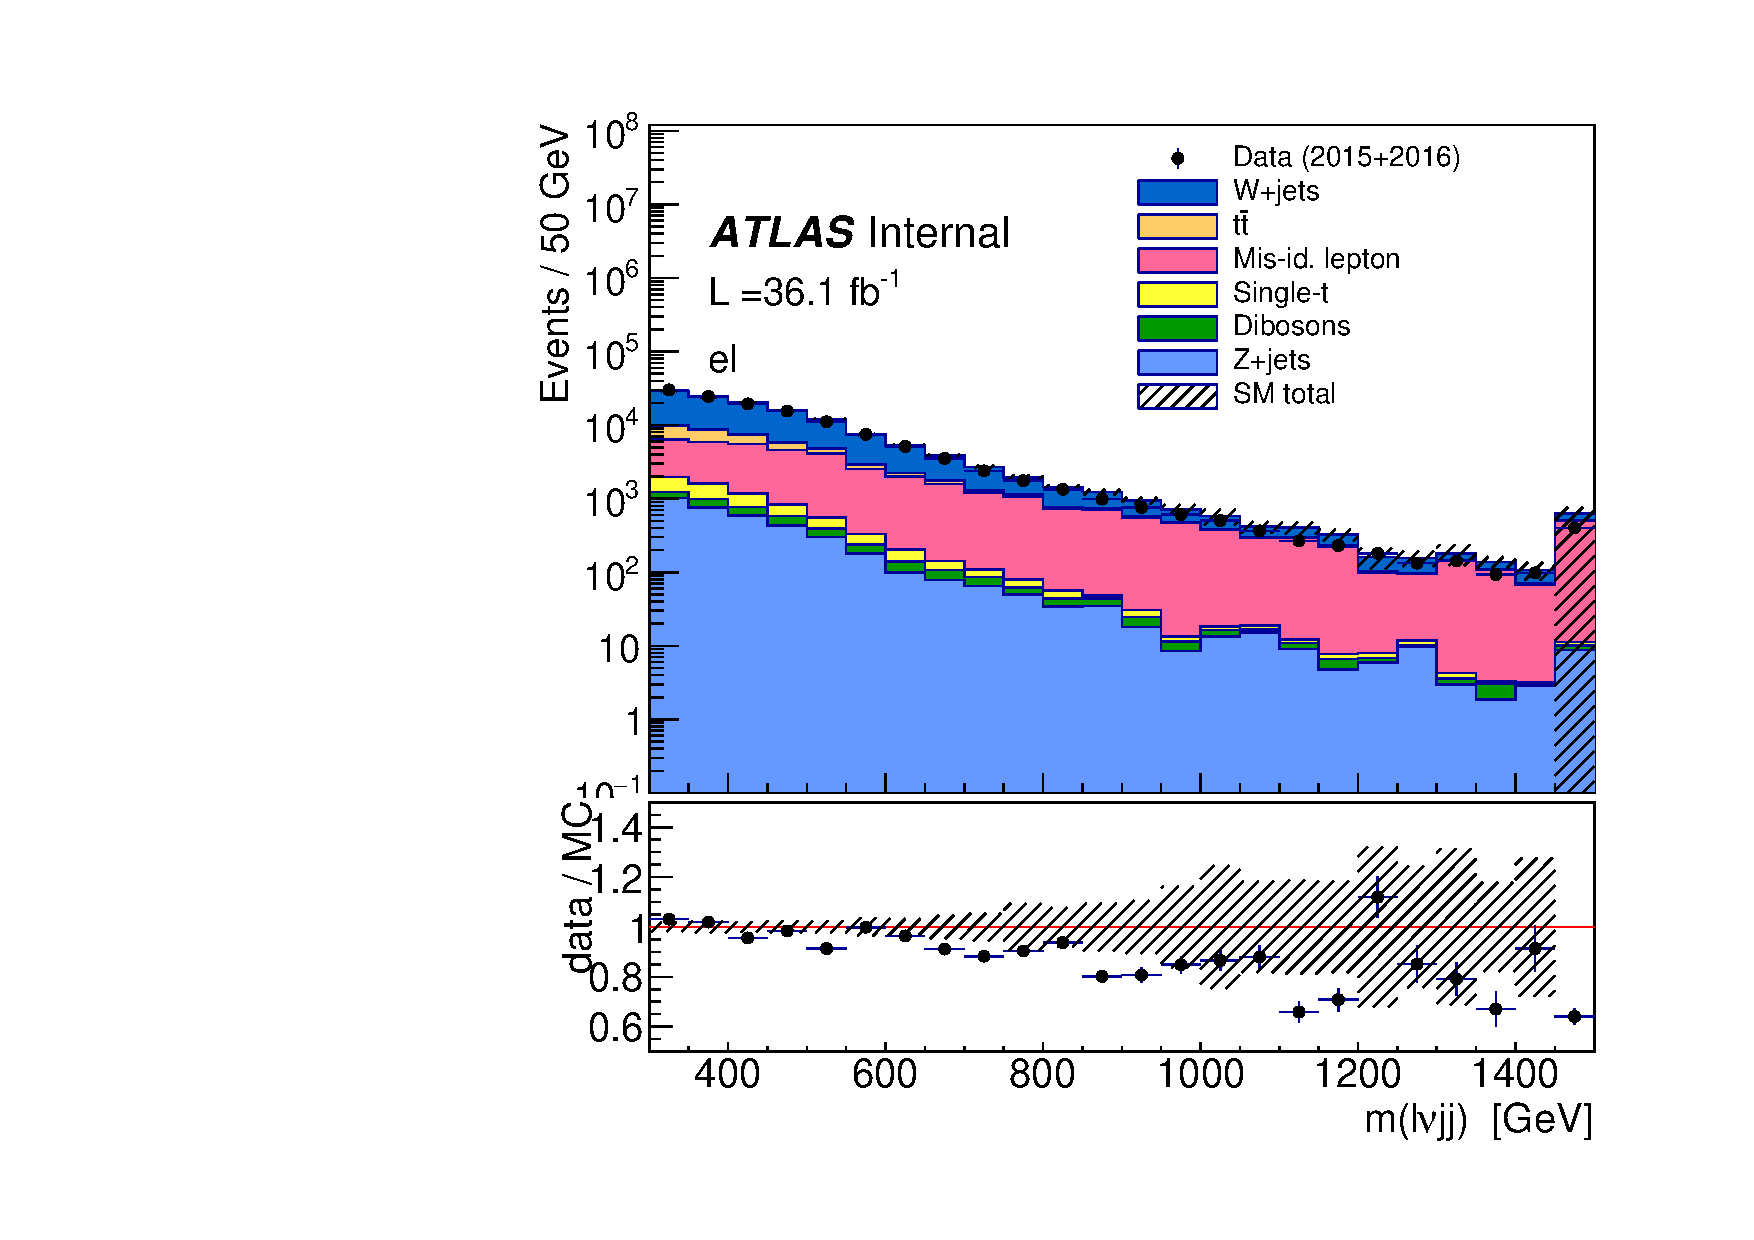
\includegraphics[width=0.43\textwidth]{Chapter3/MJ_VR/lvjjmass_Loose_el_highWpt}}
	\caption{The distribution of lepton $p_{T}$,$\eta$, $E_{T}^{miss}$, $\Delta\phi$(e,$E_{T}^{miss}$), $m_{WV}$in validation region with $p_{T}(l\nu)>150 GeV$ in electron channel with multijet background}
	\label{fig:FakeVR1_el}
	
\end{figure}
\clearpage
\begin{figure}[ht]
	\centering
	\subfloat[]{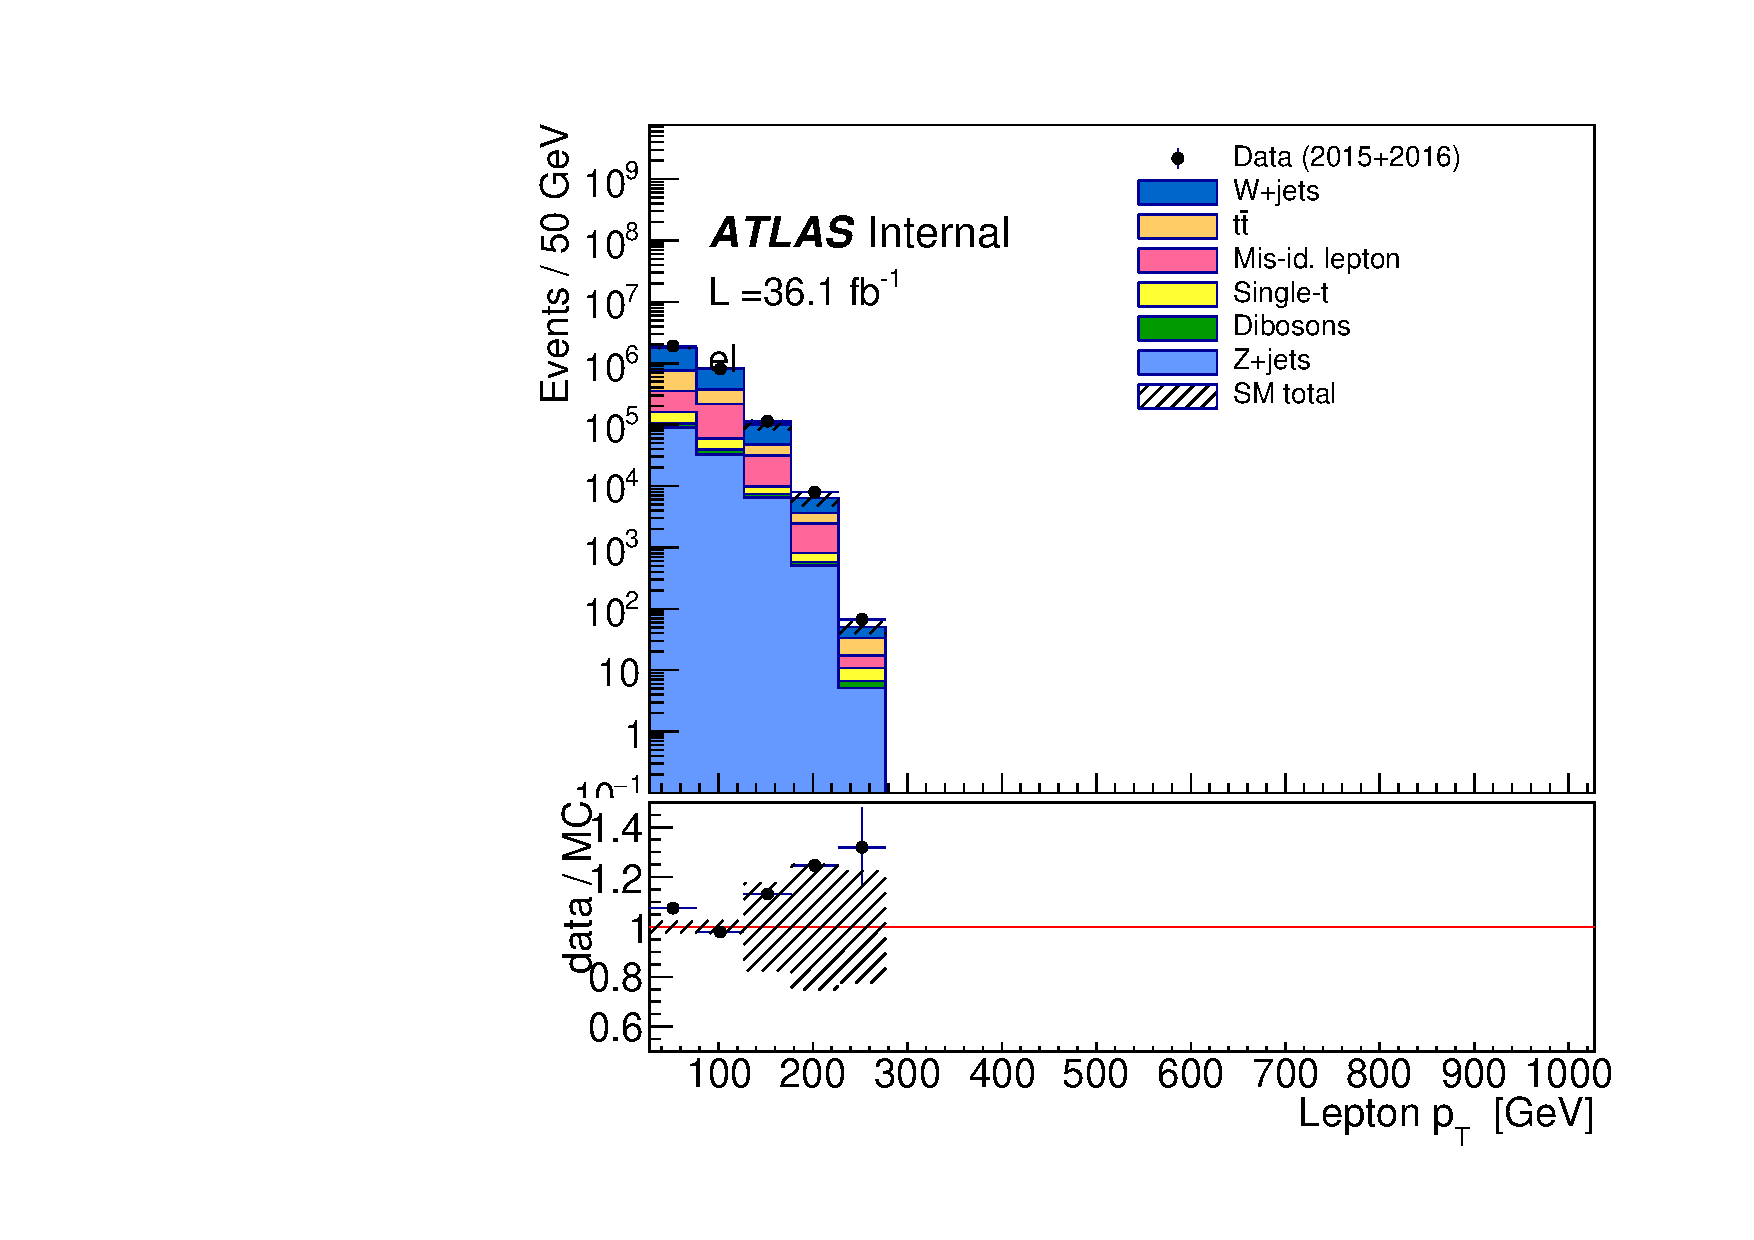
\includegraphics[width=0.43\textwidth]{Chapter3/MJ_VR/lep1pt_Loose_el_lowWpt}}
	\subfloat[]{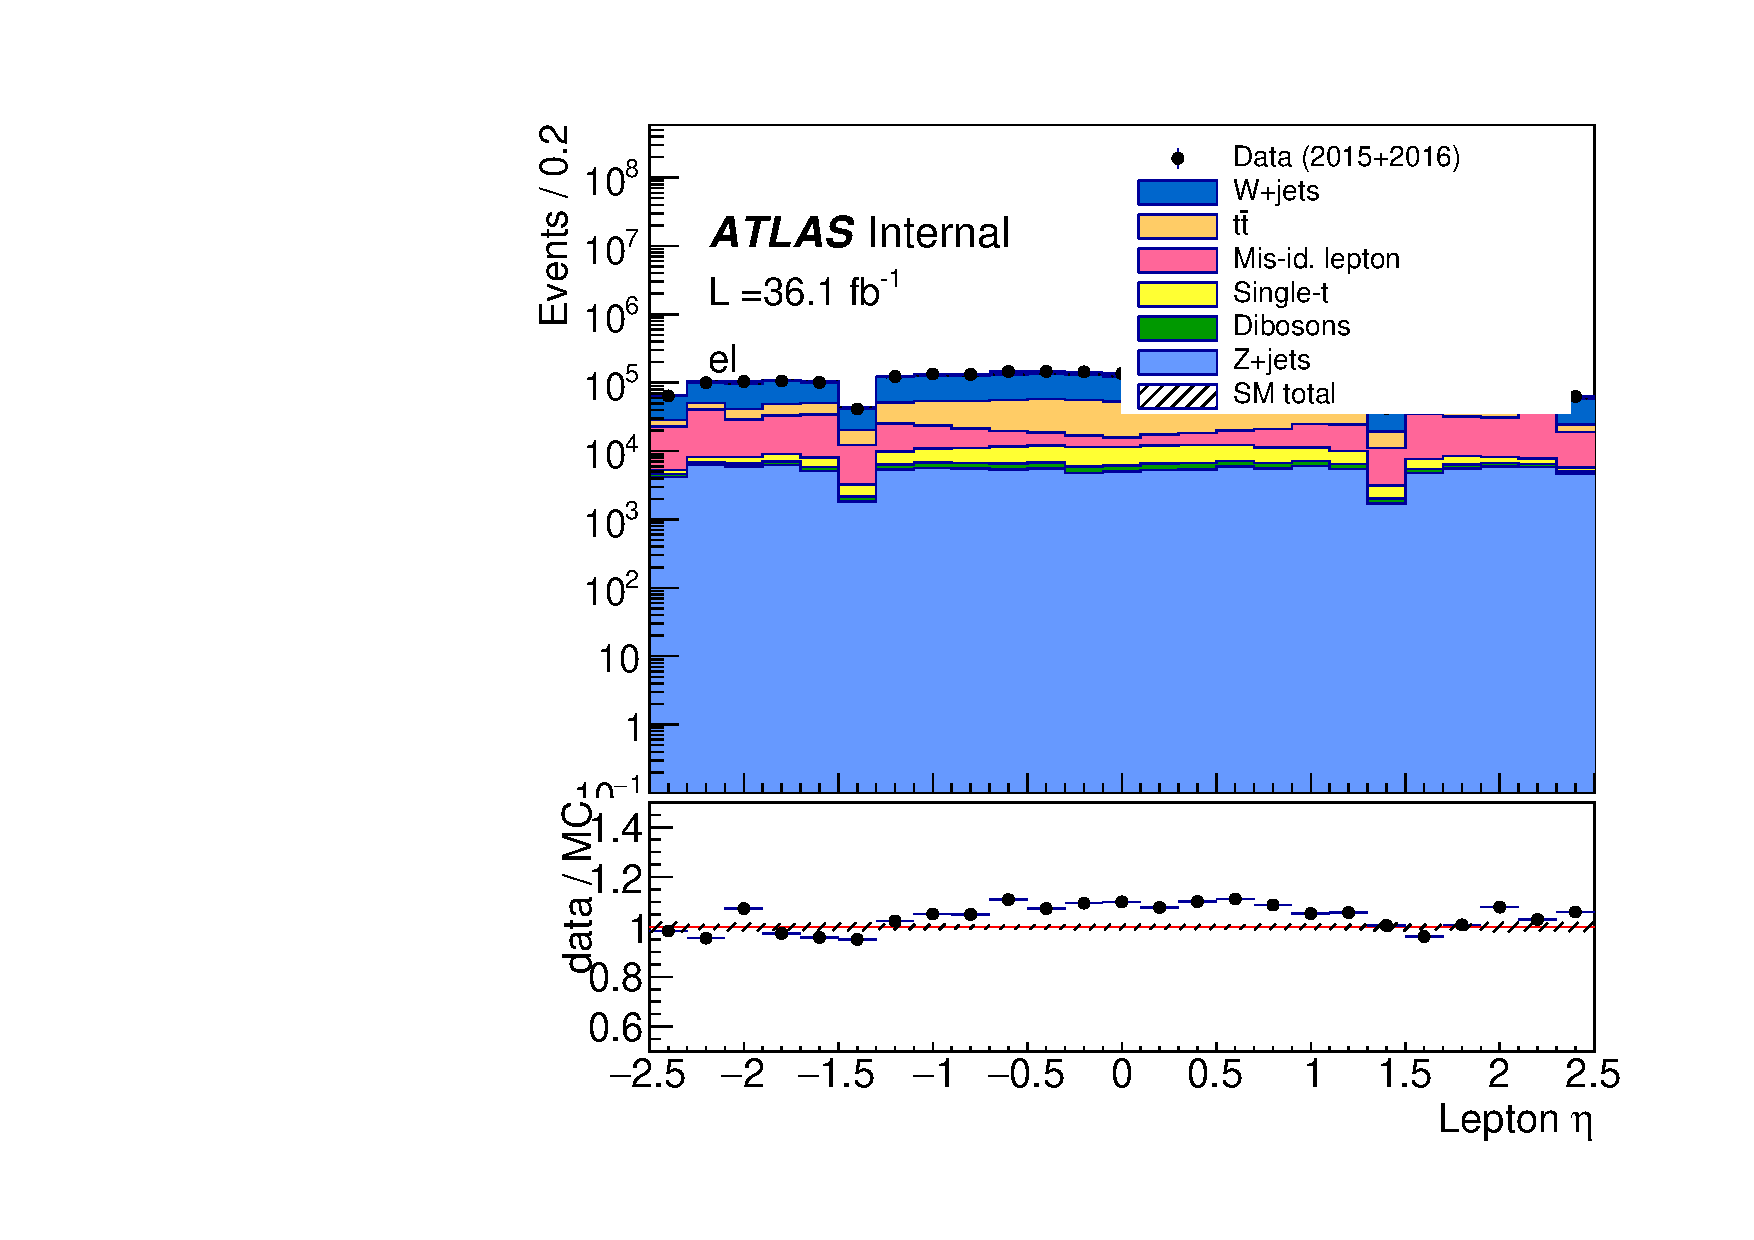
\includegraphics[width=0.43\textwidth]{Chapter3/MJ_VR/lep1eta_Loose_el_lowWpt}}\\
	\subfloat[]{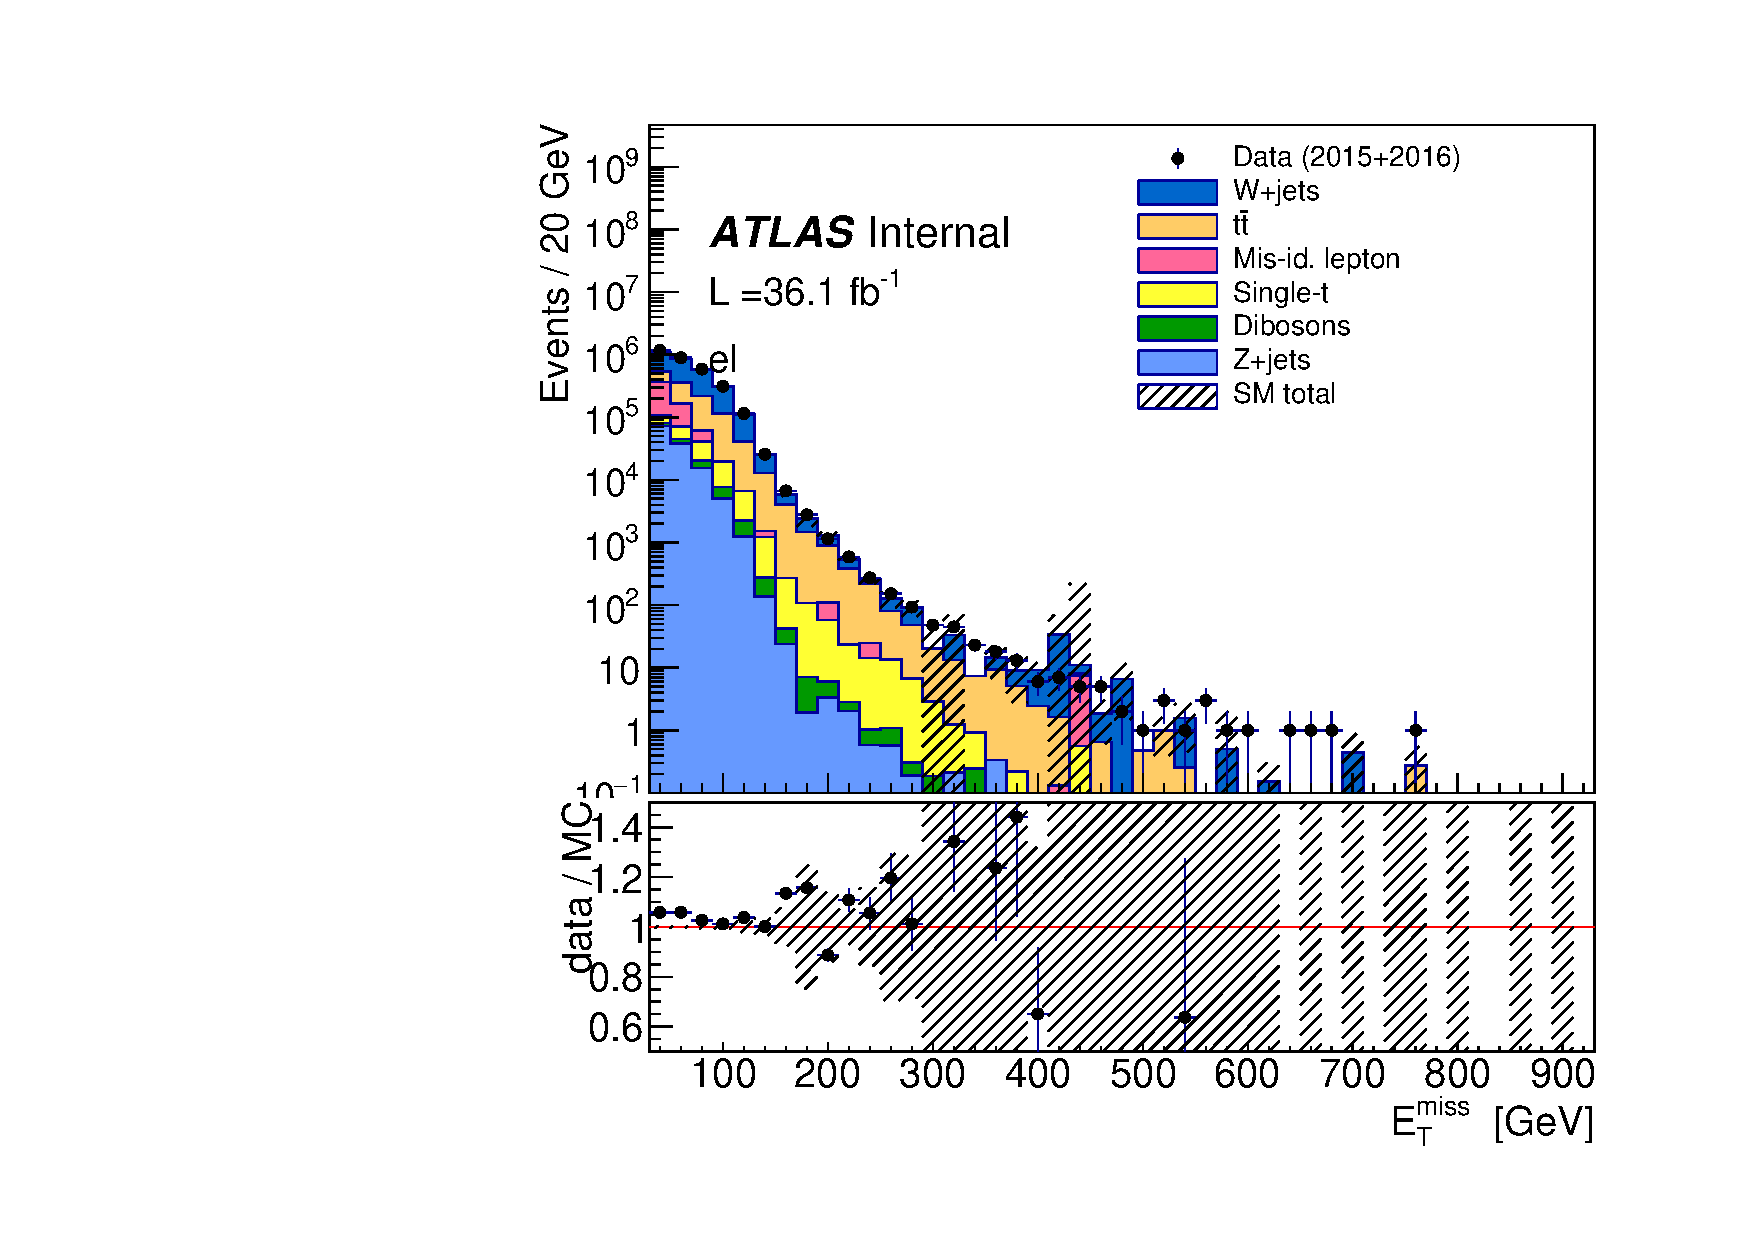
\includegraphics[width=0.43\textwidth]{Chapter3/MJ_VR/met_Loose_el_lowWpt}}
	\subfloat[]{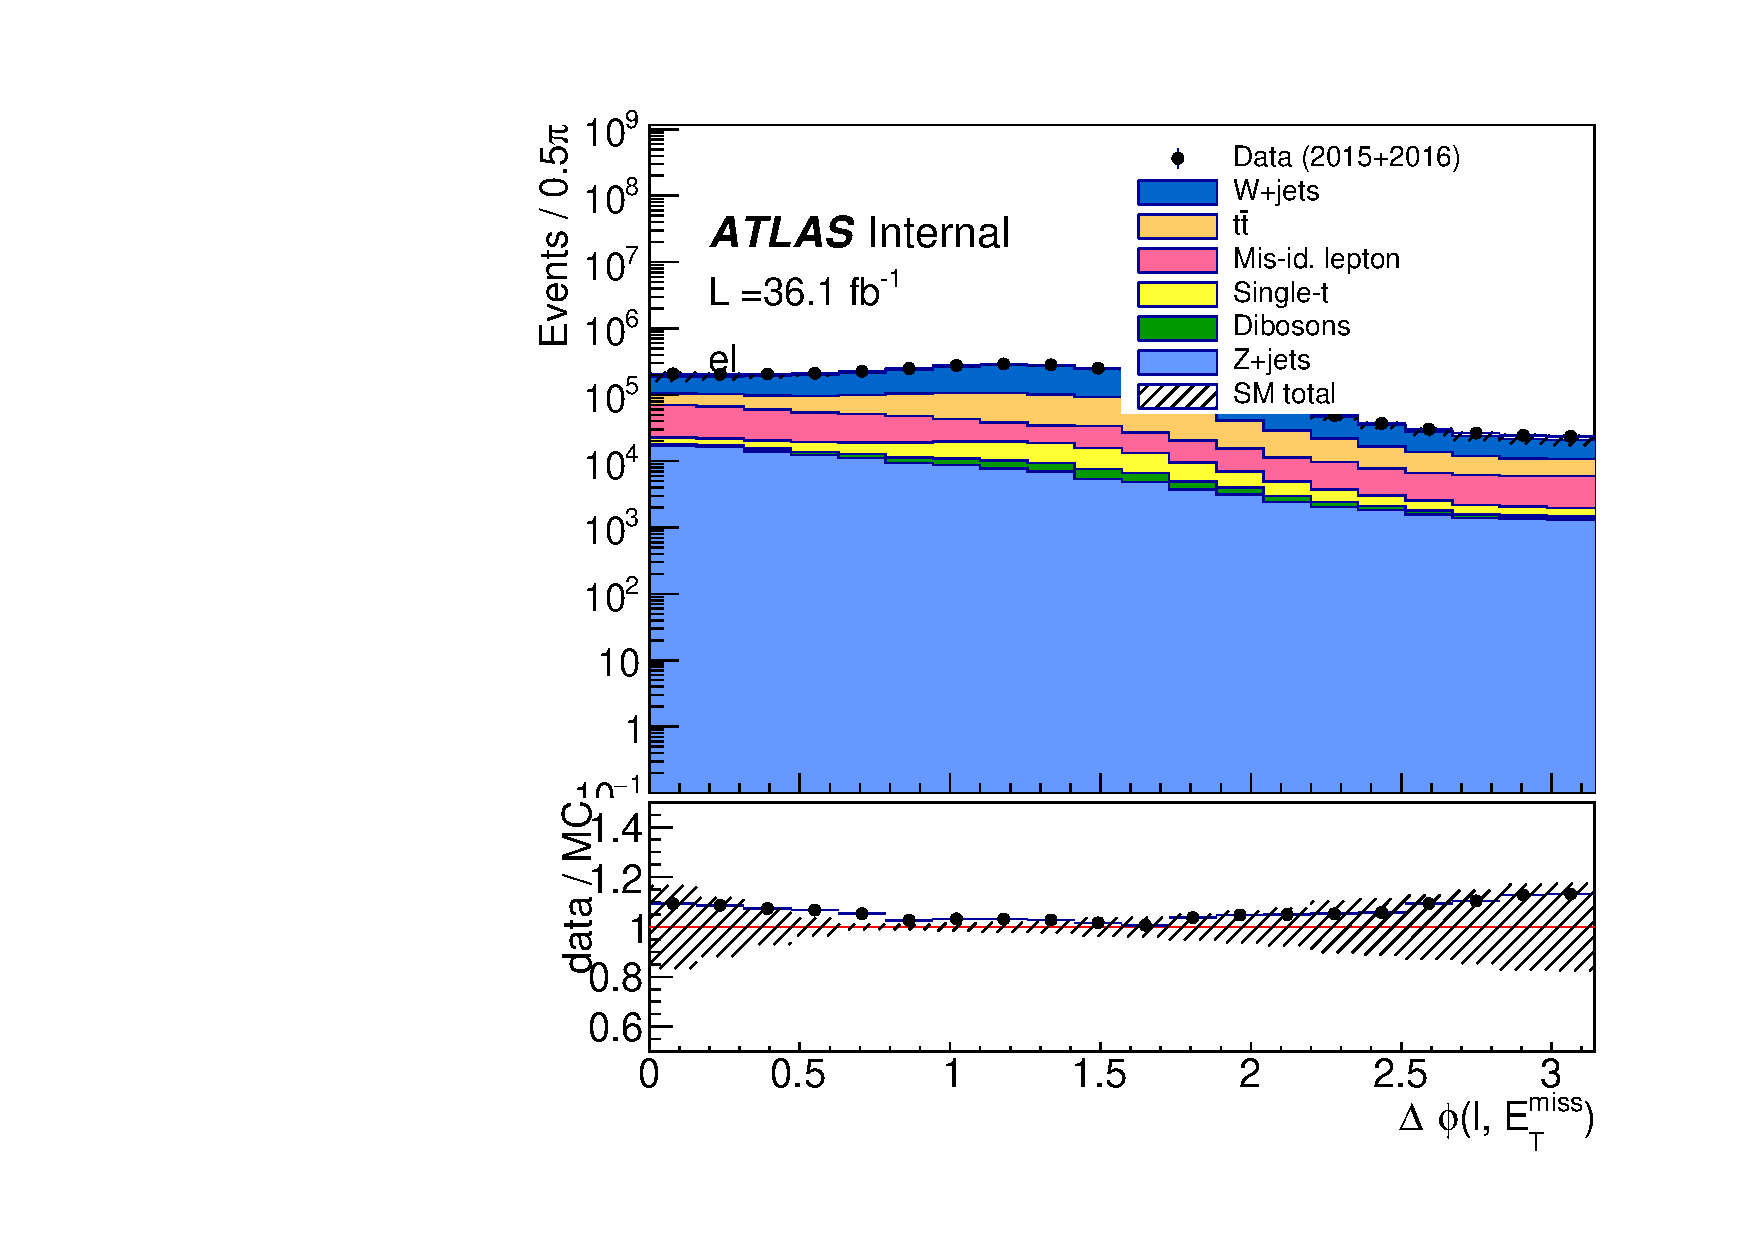
\includegraphics[width=0.43\textwidth]{Chapter3/MJ_VR/dphilepmet_Loose_el_lowWpt}}\\
	\subfloat[]{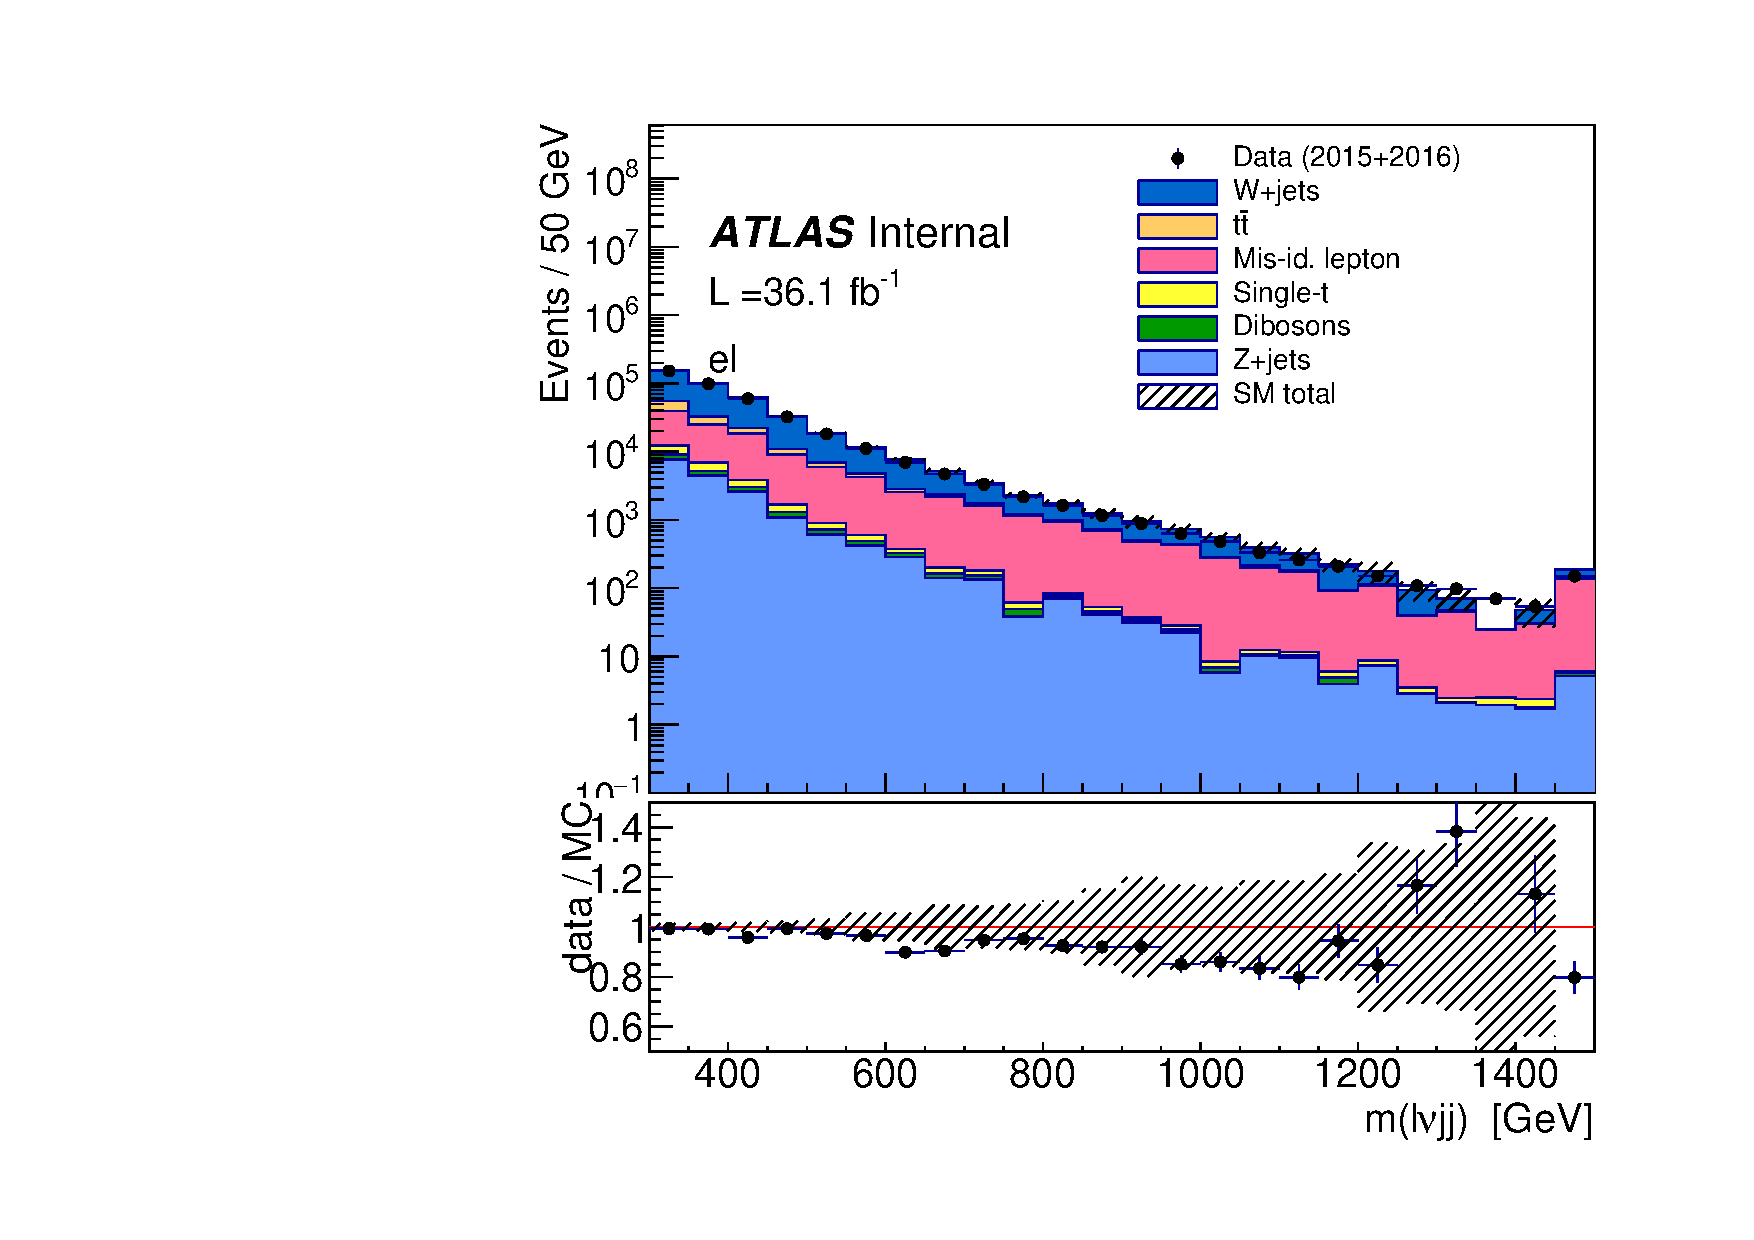
\includegraphics[width=0.43\textwidth]{Chapter3/MJ_VR/lvjjmass_Loose_el_lowWpt}}
	\caption{The distribution of lepton $p_{T}$,$\eta$, $E_{T}^{miss}$, $\Delta\phi$(e,$E_{T}^{miss}$), $m_{WV}$ and BDT in validation region with $p_{T}(l\nu)<150 GeV$ in electron channel with multijet background}
	\label{fig:FakeVR2_el}
\end{figure}
\clearpage
\begin{figure}[ht]
	\centering
	\subfloat[]{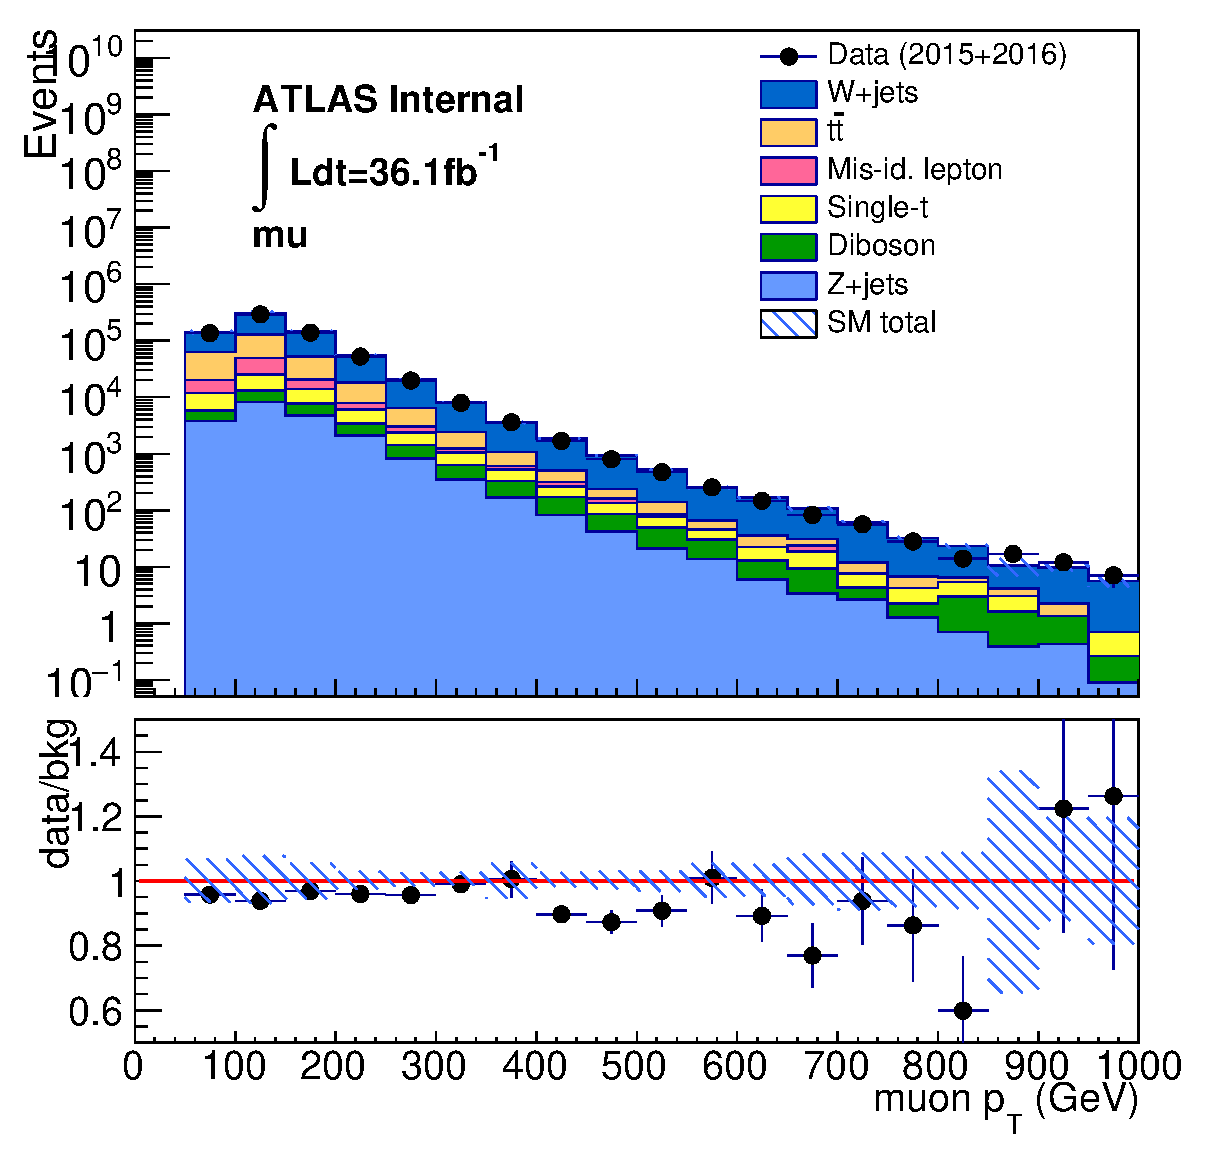
\includegraphics[width=0.43\textwidth]{Chapter3/MJ_VR/lep1pt_Loose_mu_highWpt.eps}}
	\subfloat[]{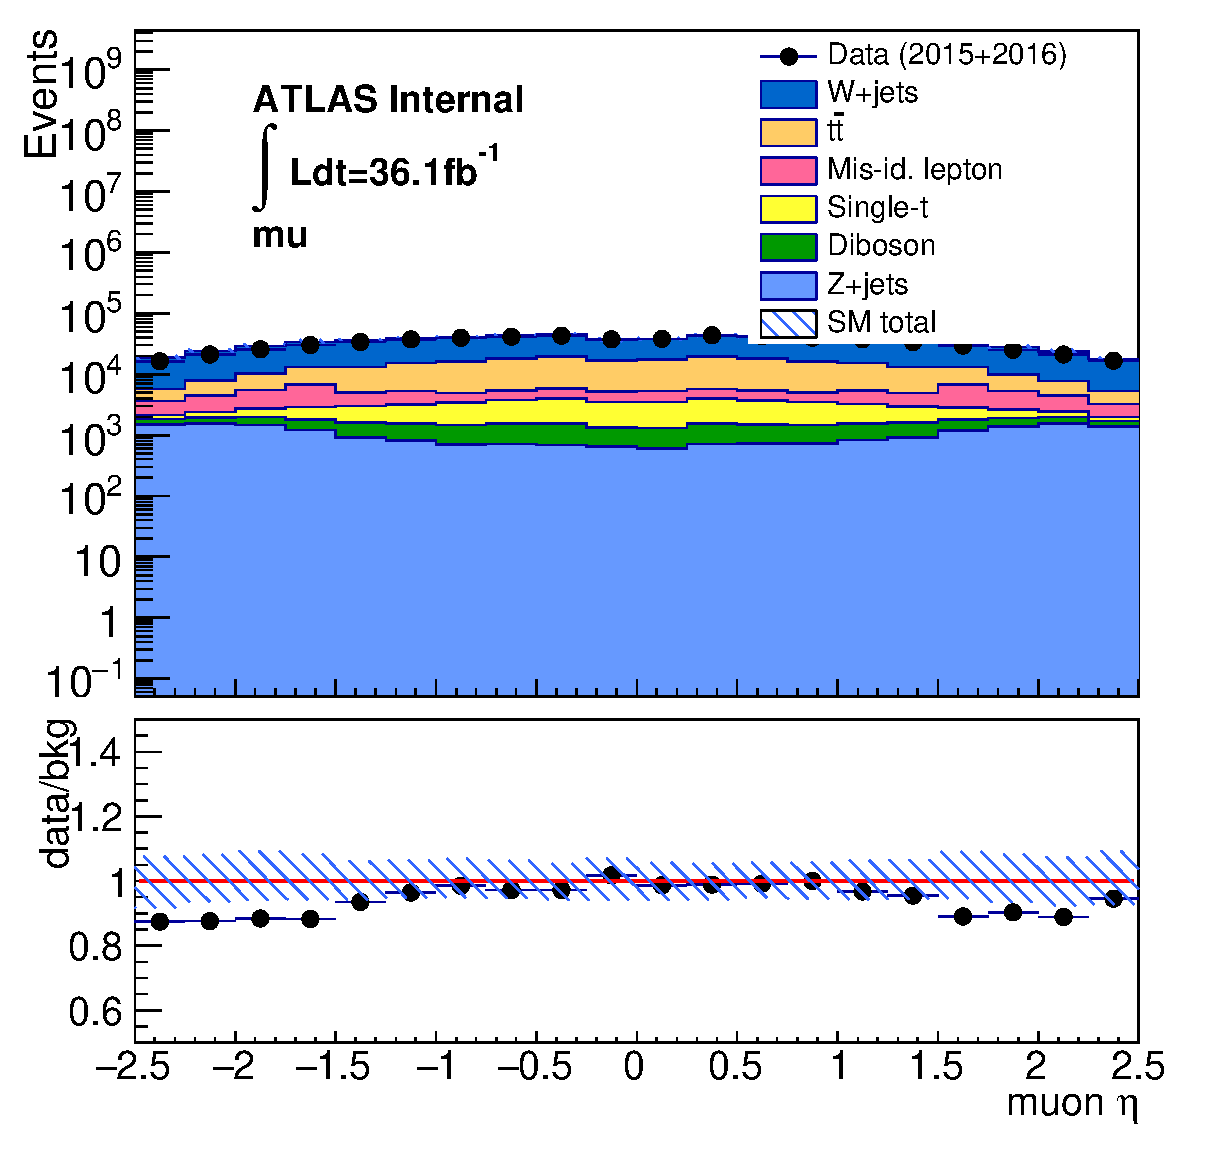
\includegraphics[width=0.43\textwidth]{Chapter3/MJ_VR/lep1eta_Loose_mu_highWpt.eps}}\\
	\subfloat[]{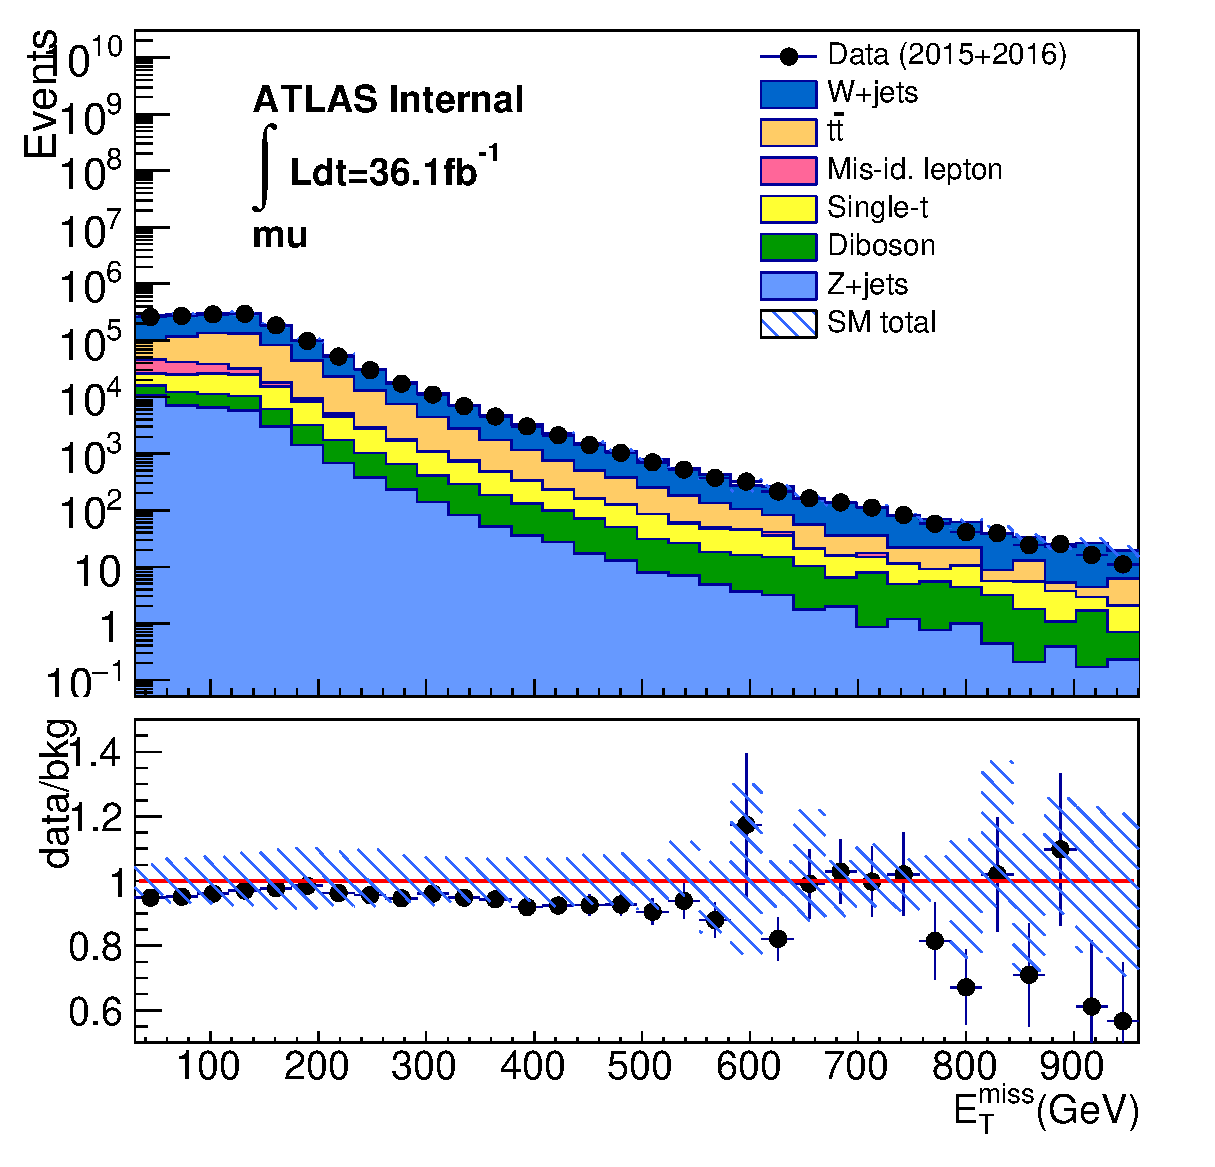
\includegraphics[width=0.43\textwidth]{Chapter3/MJ_VR/met_Loose_mu_highWpt.eps}}
	\subfloat[]{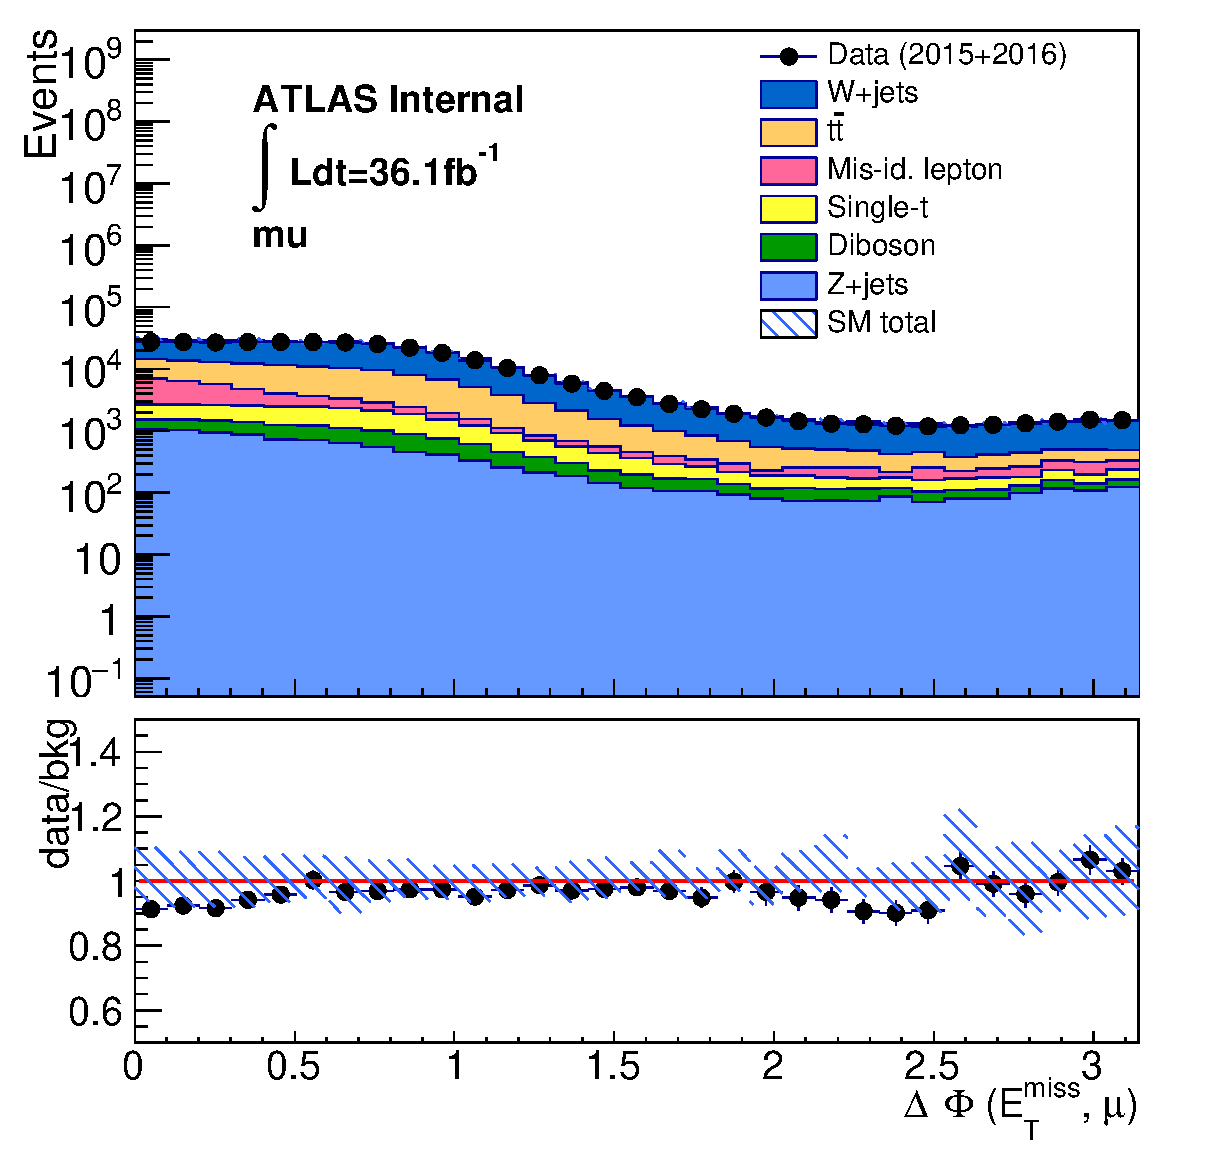
\includegraphics[width=0.43\textwidth]{Chapter3/MJ_VR/dphilepmet_Loose_mu_highWpt.eps}}\\
	\subfloat[]{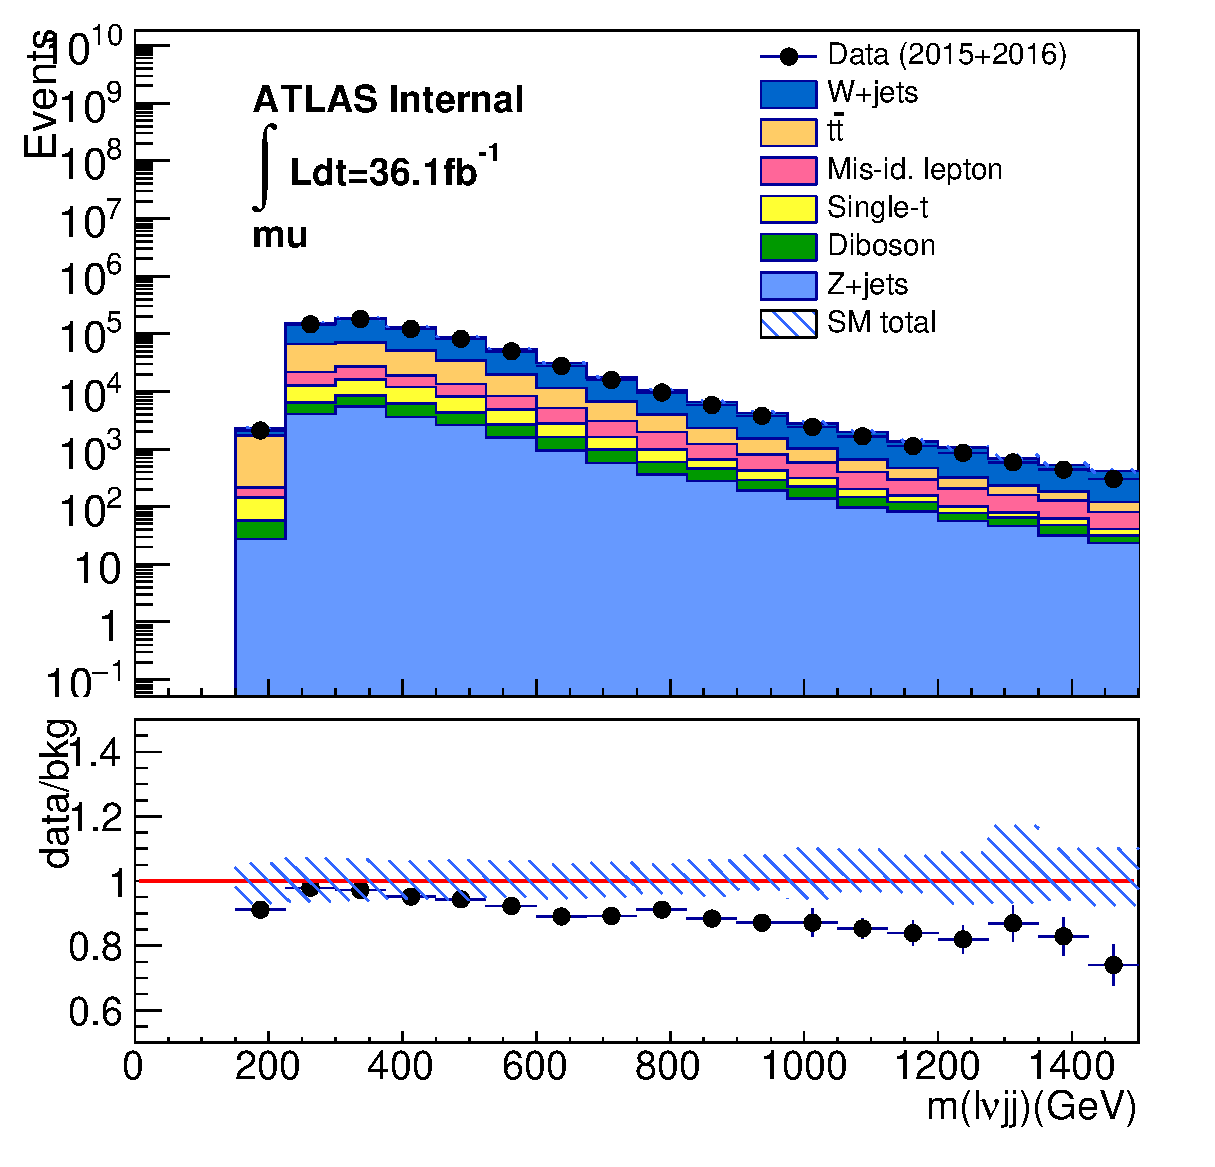
\includegraphics[width=0.43\textwidth]{Chapter3/MJ_VR/lvjjmass_Loose_mu_highWpt.eps}}
	\caption{The distribution of lepton $p_{T}$,$\eta$, $E_{T}^{miss}$, $\Delta\phi$($\mu$,$E_{T}^{miss}$), $m_{WV}$ and BDT in validation region with $p_{T}(l\nu)>150 GeV$ in muon channel with multijet background}
	\label{fig:FakeVR1_mu}
\end{figure}
\clearpage
\begin{figure}[ht]
	\centering
	\subfloat[]{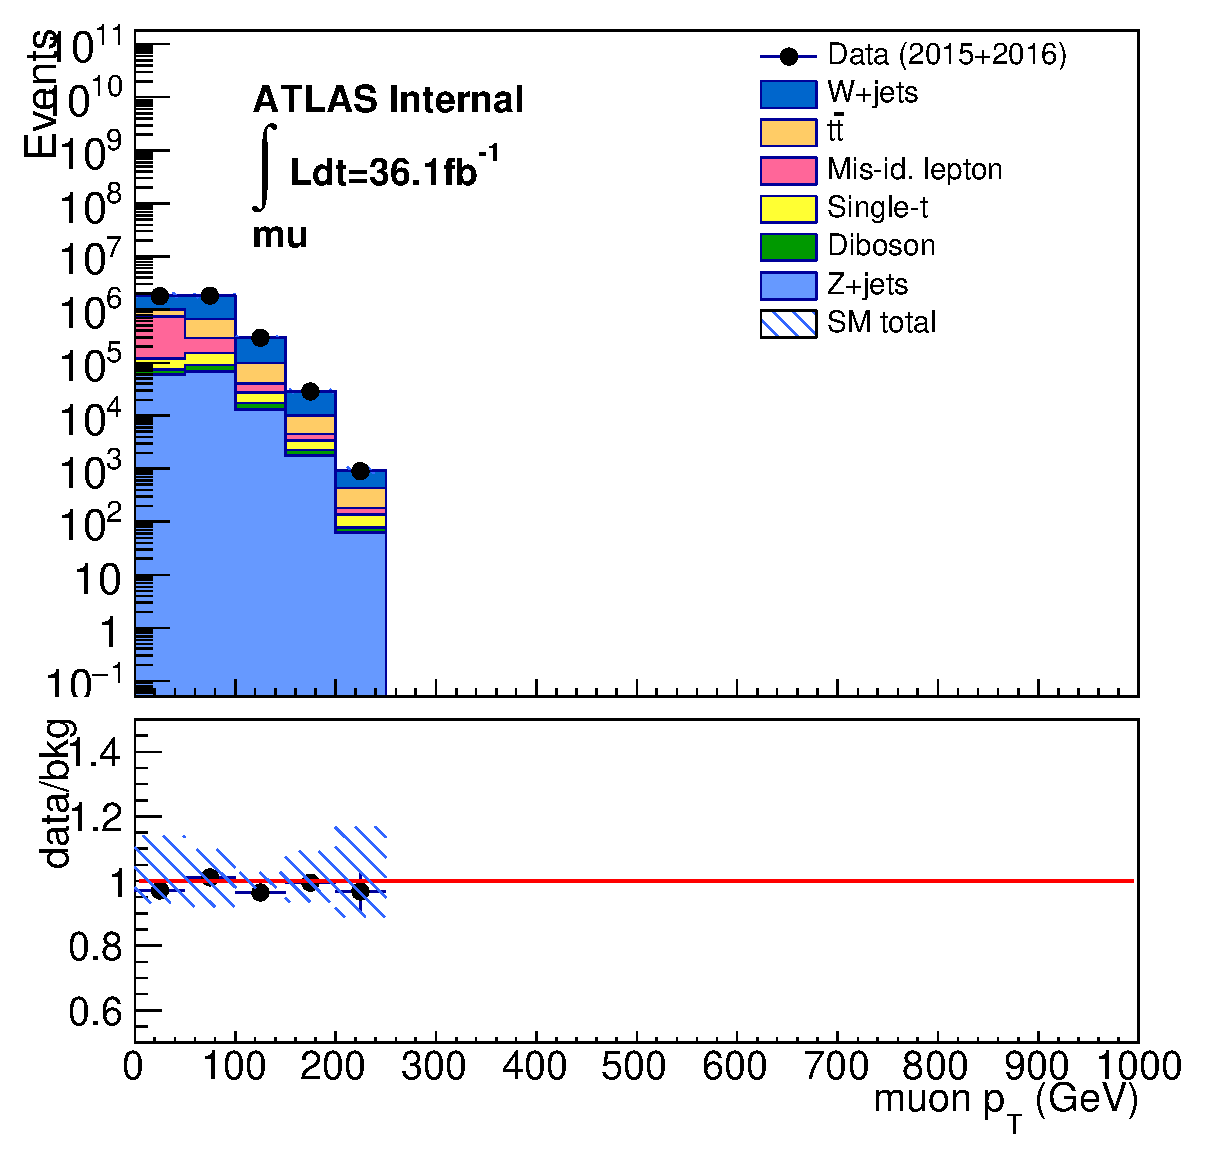
\includegraphics[width=0.43\textwidth]{Chapter3/MJ_VR/lep1pt_Loose_mu_lowWpt.eps}}
	\subfloat[]{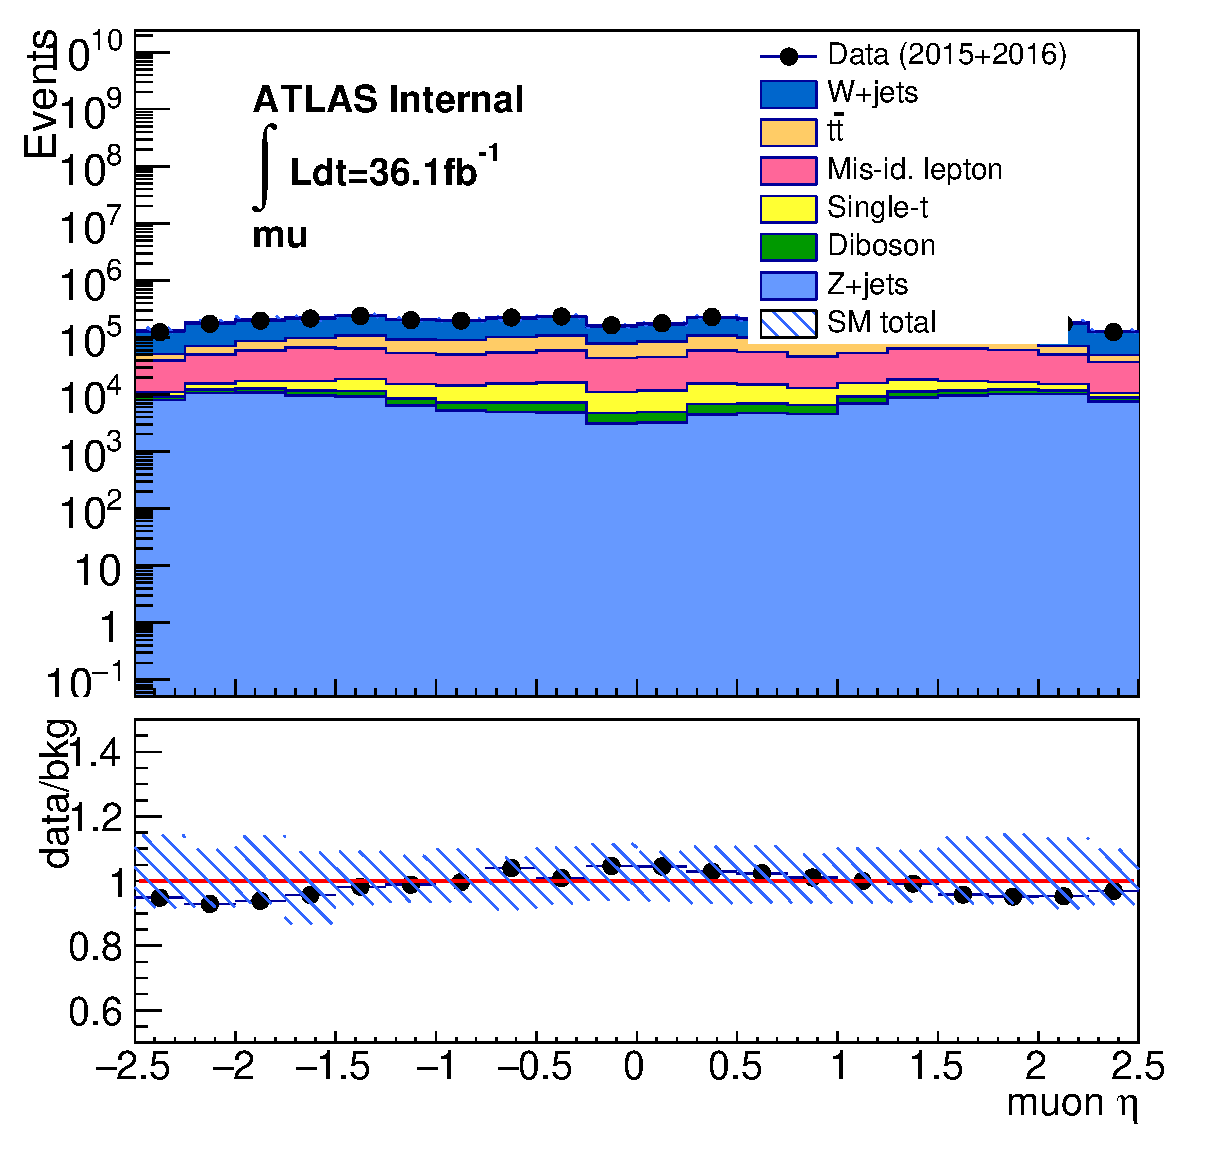
\includegraphics[width=0.43\textwidth]{Chapter3/MJ_VR/lep1eta_Loose_mu_lowWpt.eps}}\\
	\subfloat[]{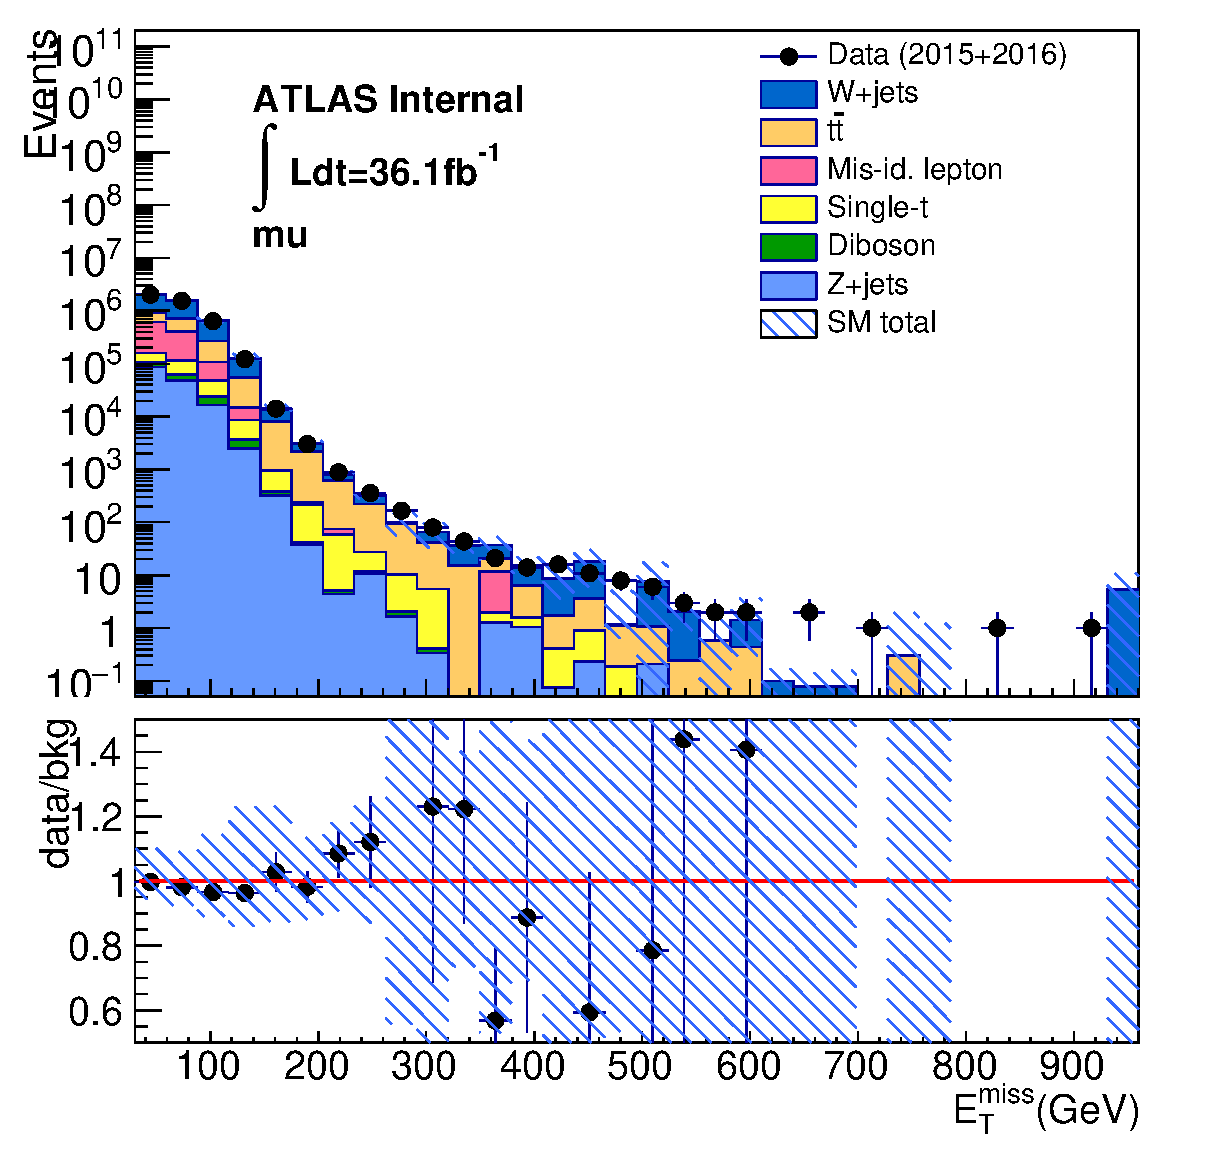
\includegraphics[width=0.43\textwidth]{Chapter3/MJ_VR/met_Loose_mu_lowWpt.eps}}
	\subfloat[]{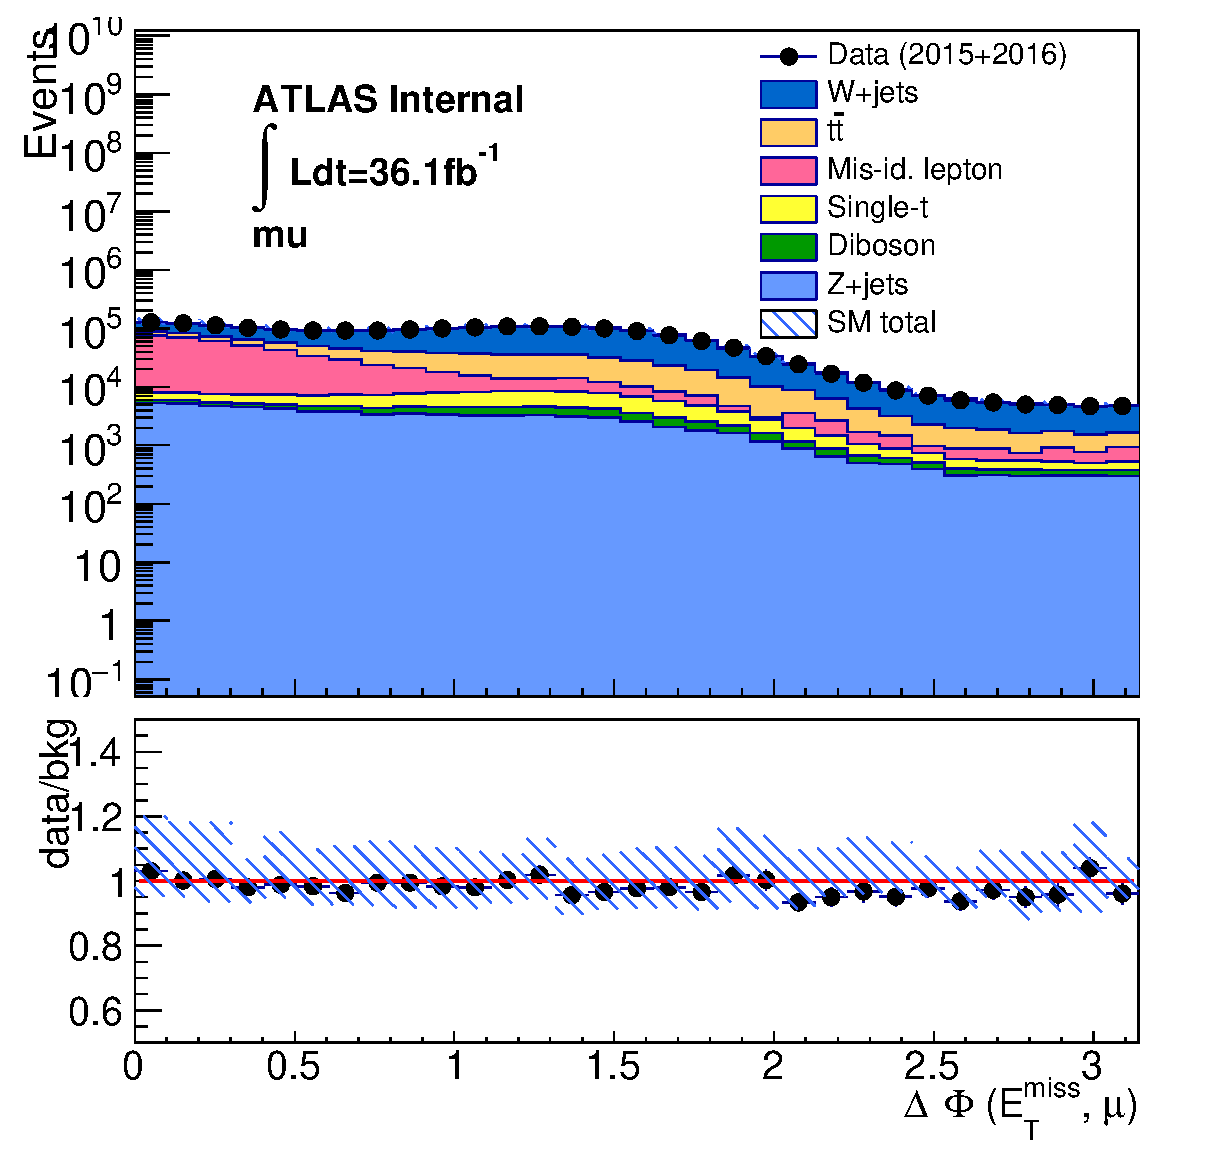
\includegraphics[width=0.43\textwidth]{Chapter3/MJ_VR/dphilepmet_Loose_mu_lowWpt.eps}}\\
	\subfloat[]{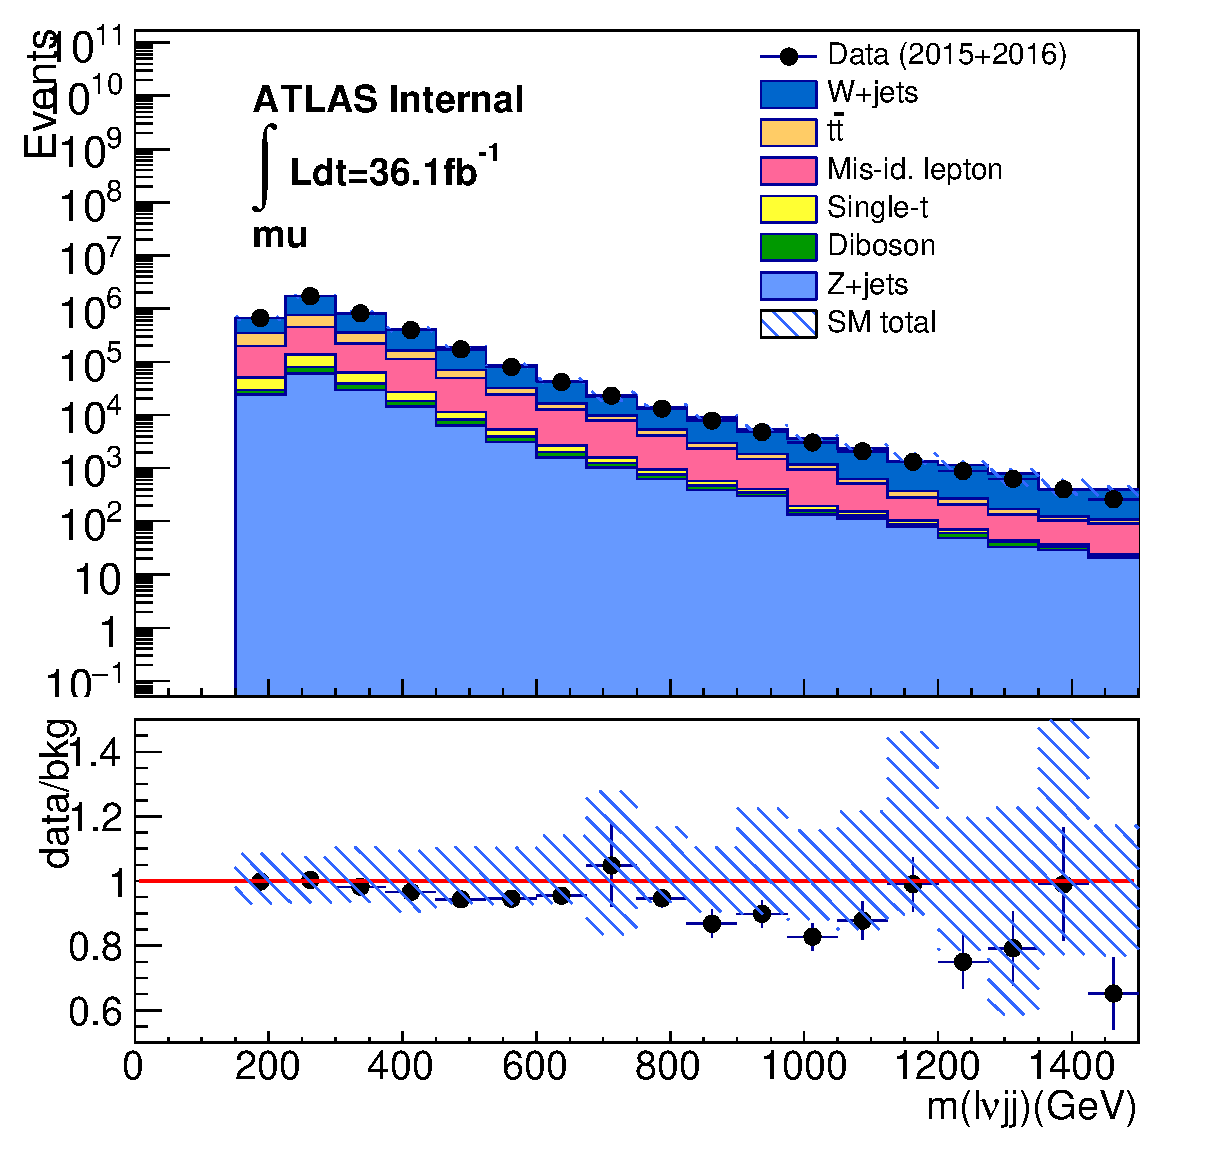
\includegraphics[width=0.43\textwidth]{Chapter3/MJ_VR/lvjjmass_Loose_mu_lowWpt.eps}}
	\caption{The distribution of lepton $p_{T}$,$\eta$, $E_{T}^{miss}$, $\Delta\phi$($\mu$,$E_{T}^{miss}$), $m_{WV}$ and BDT in validation region with $p_{T}(l\nu)<150 GeV$ in muon channel with multijet background}
	\label{fig:FakeVR2_mu}
\end{figure}
\clearpage
\section{Data Background Comparison}
\label{Sec:data_bkg_compar}
To verify the modelling of background estimation, the comparison in top and W+jet control regions are performed for both VBF and ggF categories. The consistency is not perfect as expectation, and the fitting in the control regions is on the purpose to recover it, which will be discussed in next chapter. The other issue in the background simulation is that a slope in the ratio of data over background is observed in $m^{VBF}_{jj}$ in resolved VBF category for V+jet samples from Sherpa generator. In this analysis, it is also taken as one contribution to the mismodelling of simulation. 
\\
\\Fig. \ref{Fig:ggFWR} and Fig. \ref{Fig:ggFTR} are the comparison plots for $m_{WV}$ in ggF category, while Fig. \ref{Fig:mWVVBFWR} to Fig. \ref{Fig:mWVVBFTR} are for VBF category. The comparison of  $m^{VBF}(j,j)$ could be found in Fig. \ref{Fig:mJJVBFWR} and Fig. \ref{Fig:mJJVBFTR} to examine the VBF modelling. 
\newpage

\begin{figure}[ht]
	\centering
	\subfloat[]{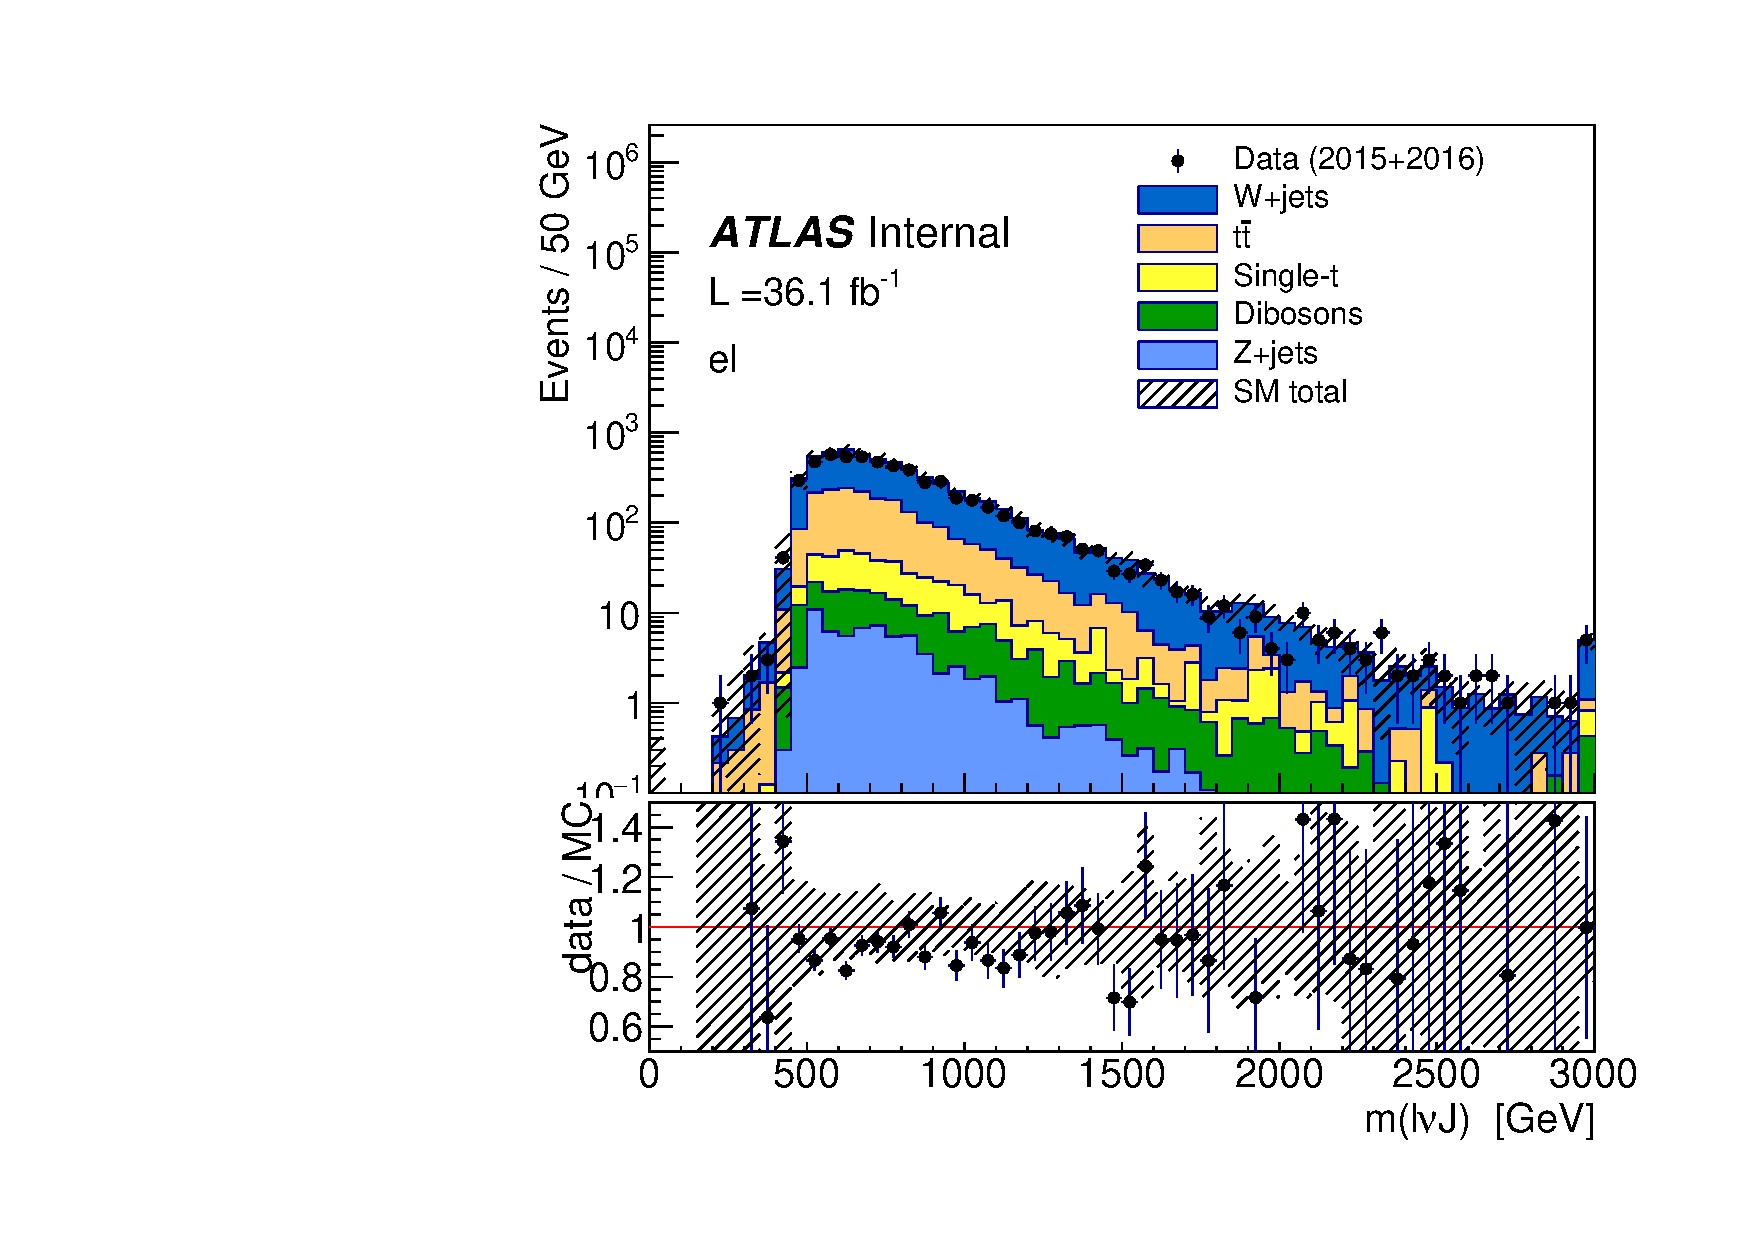
\includegraphics[width=0.43\textwidth]{Chapter3/HighPurityCR_36fb/VVM_3_el}}
	\subfloat[]{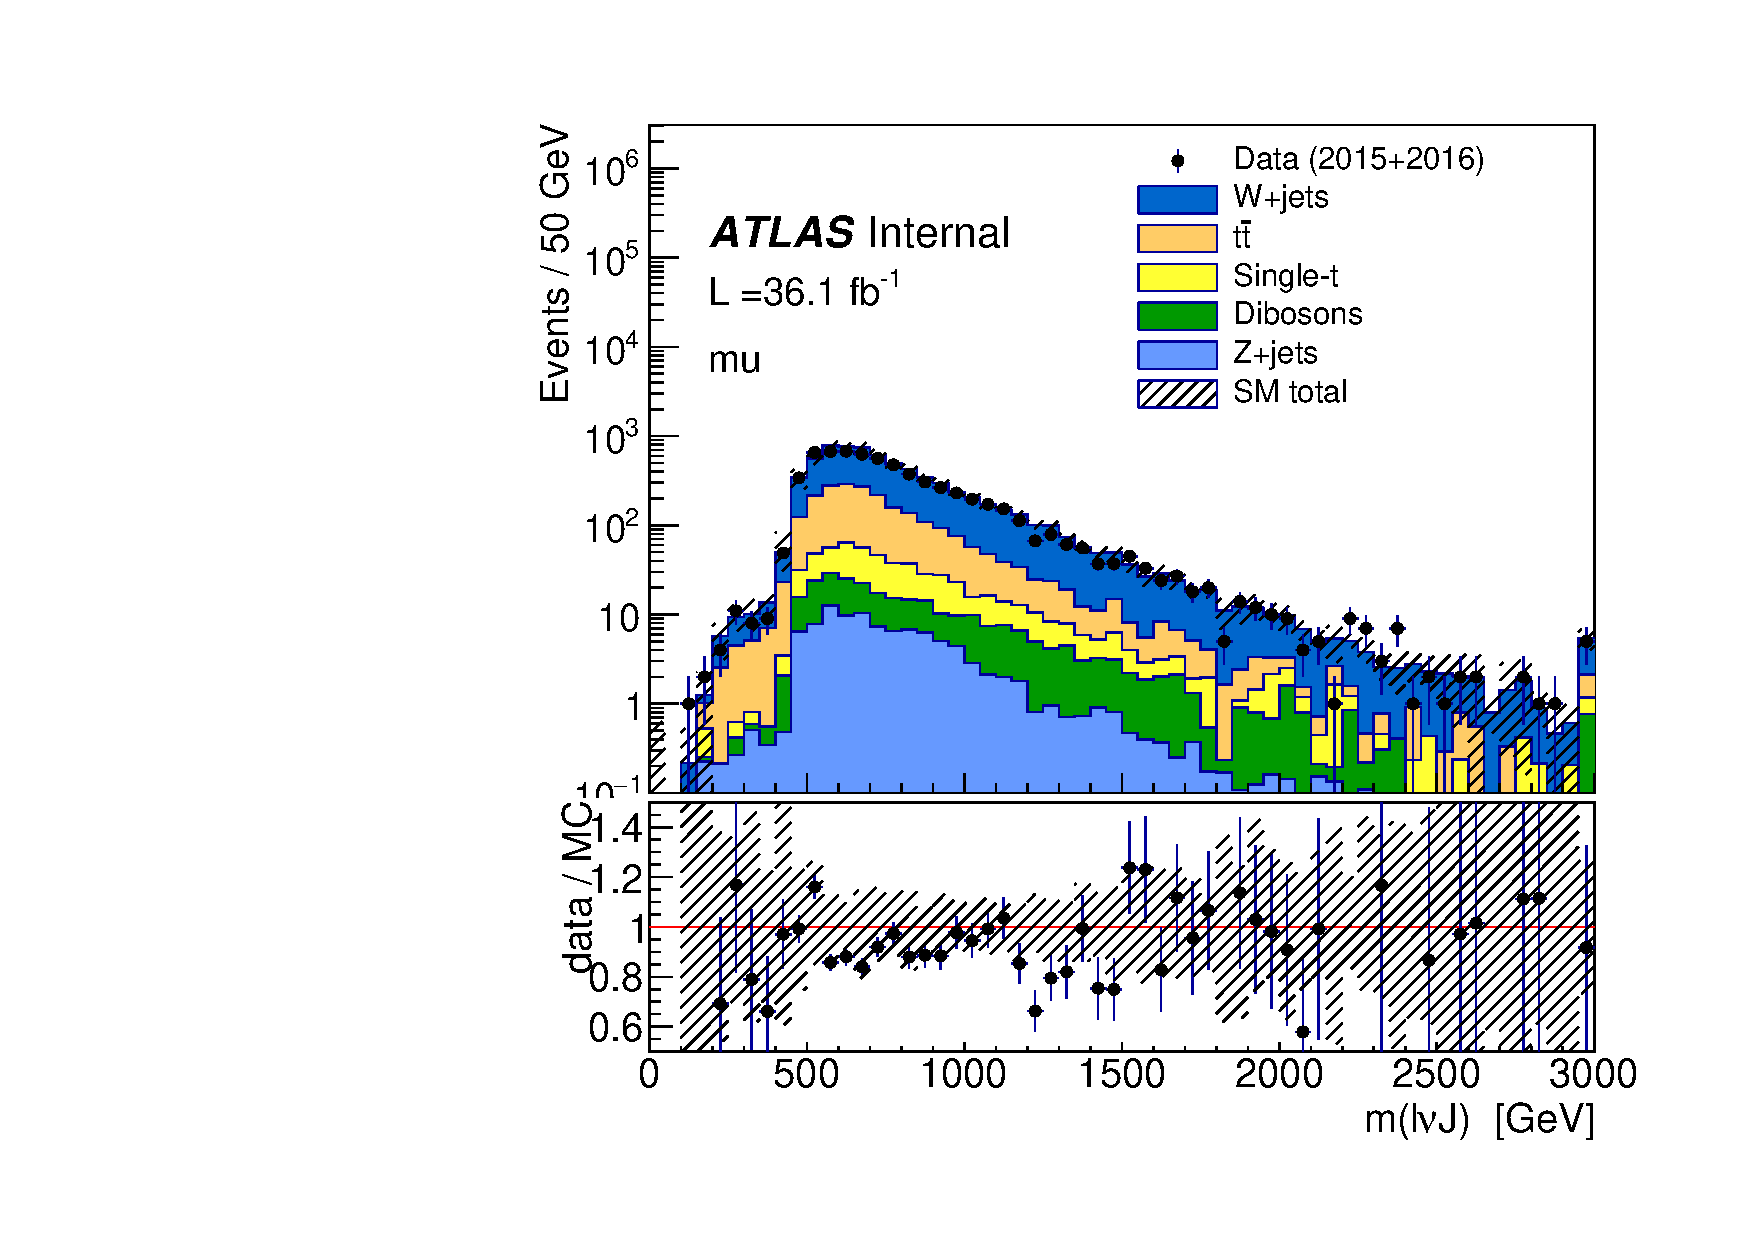
\includegraphics[width=0.43\textwidth]{Chapter3/HighPurityCR_36fb/VVM_3_mu}}\\
	\subfloat[]{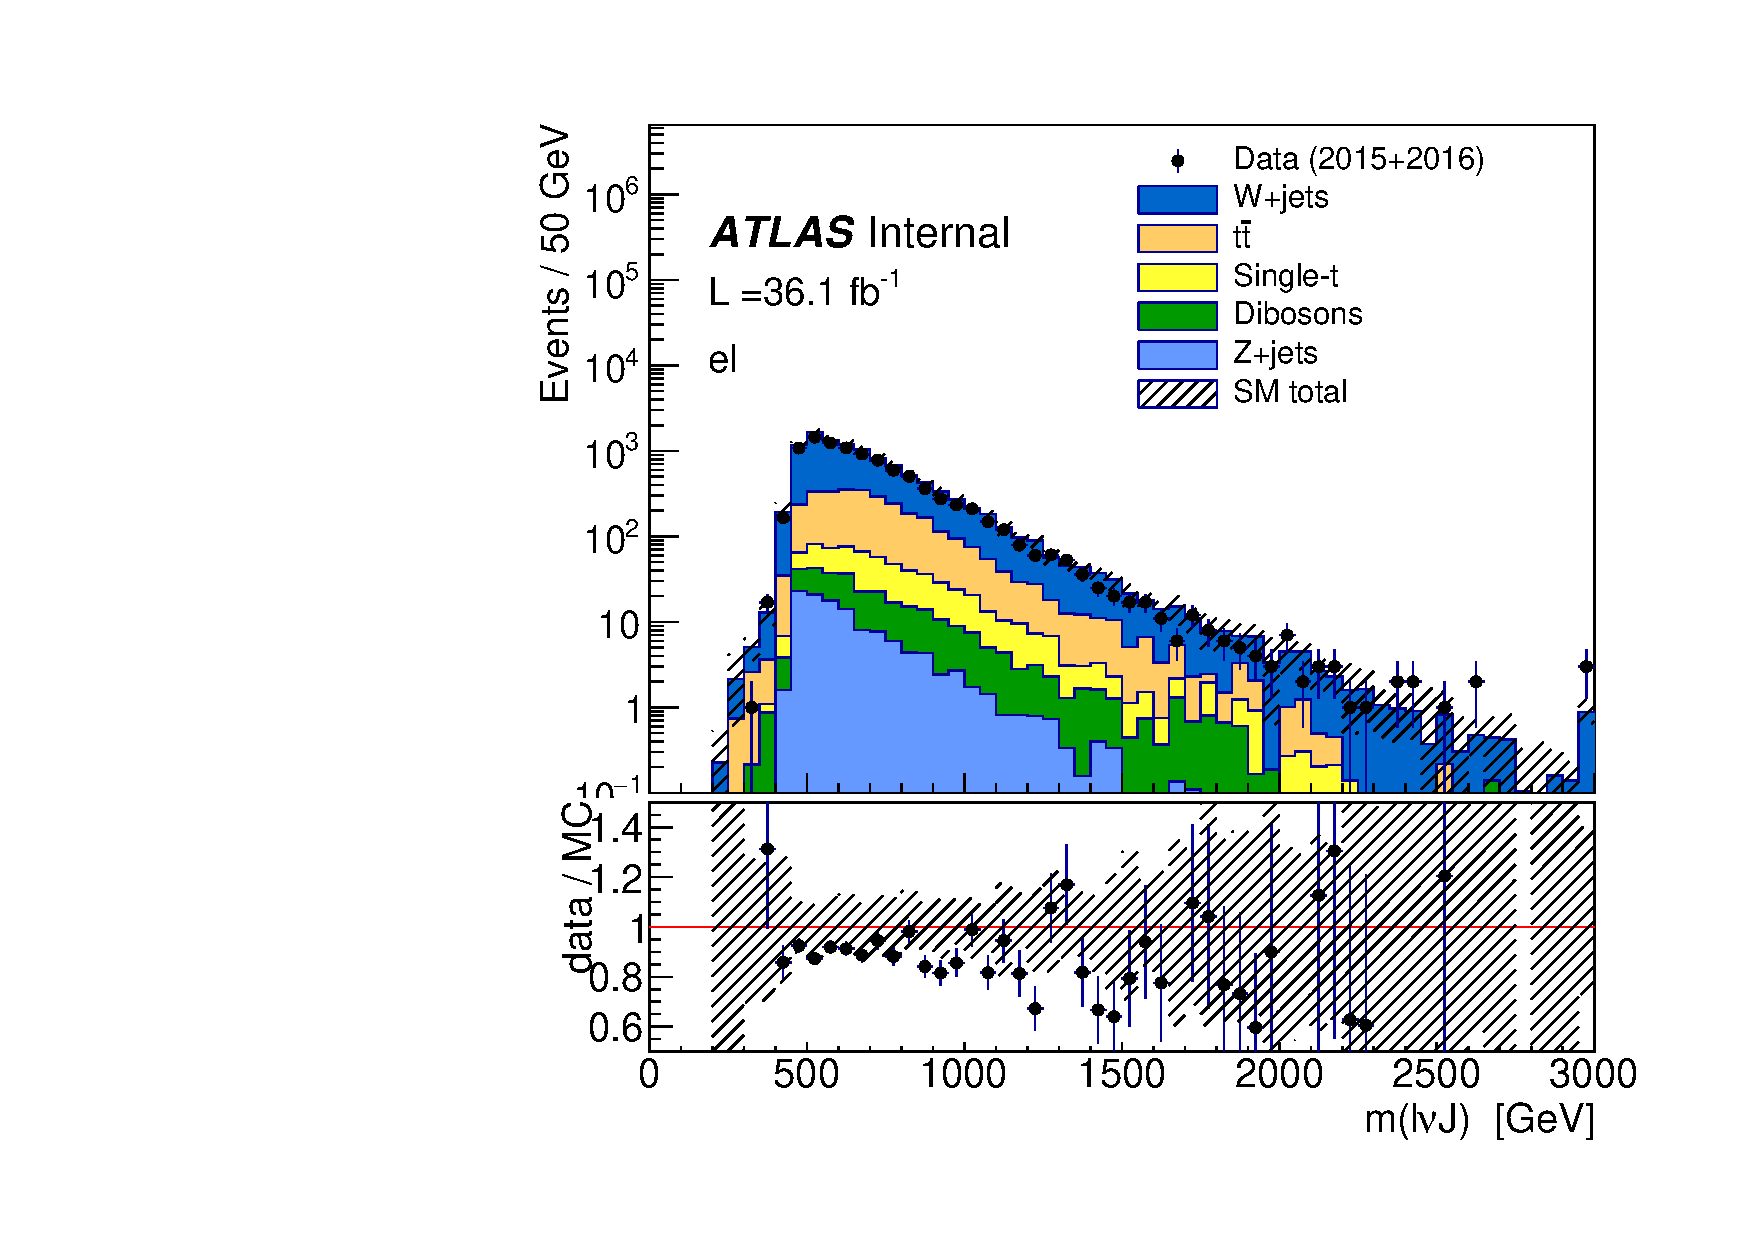
\includegraphics[width=0.43\textwidth]{Chapter3/LowPurityCR_36fb/VVM_12_el}}
	\subfloat[]{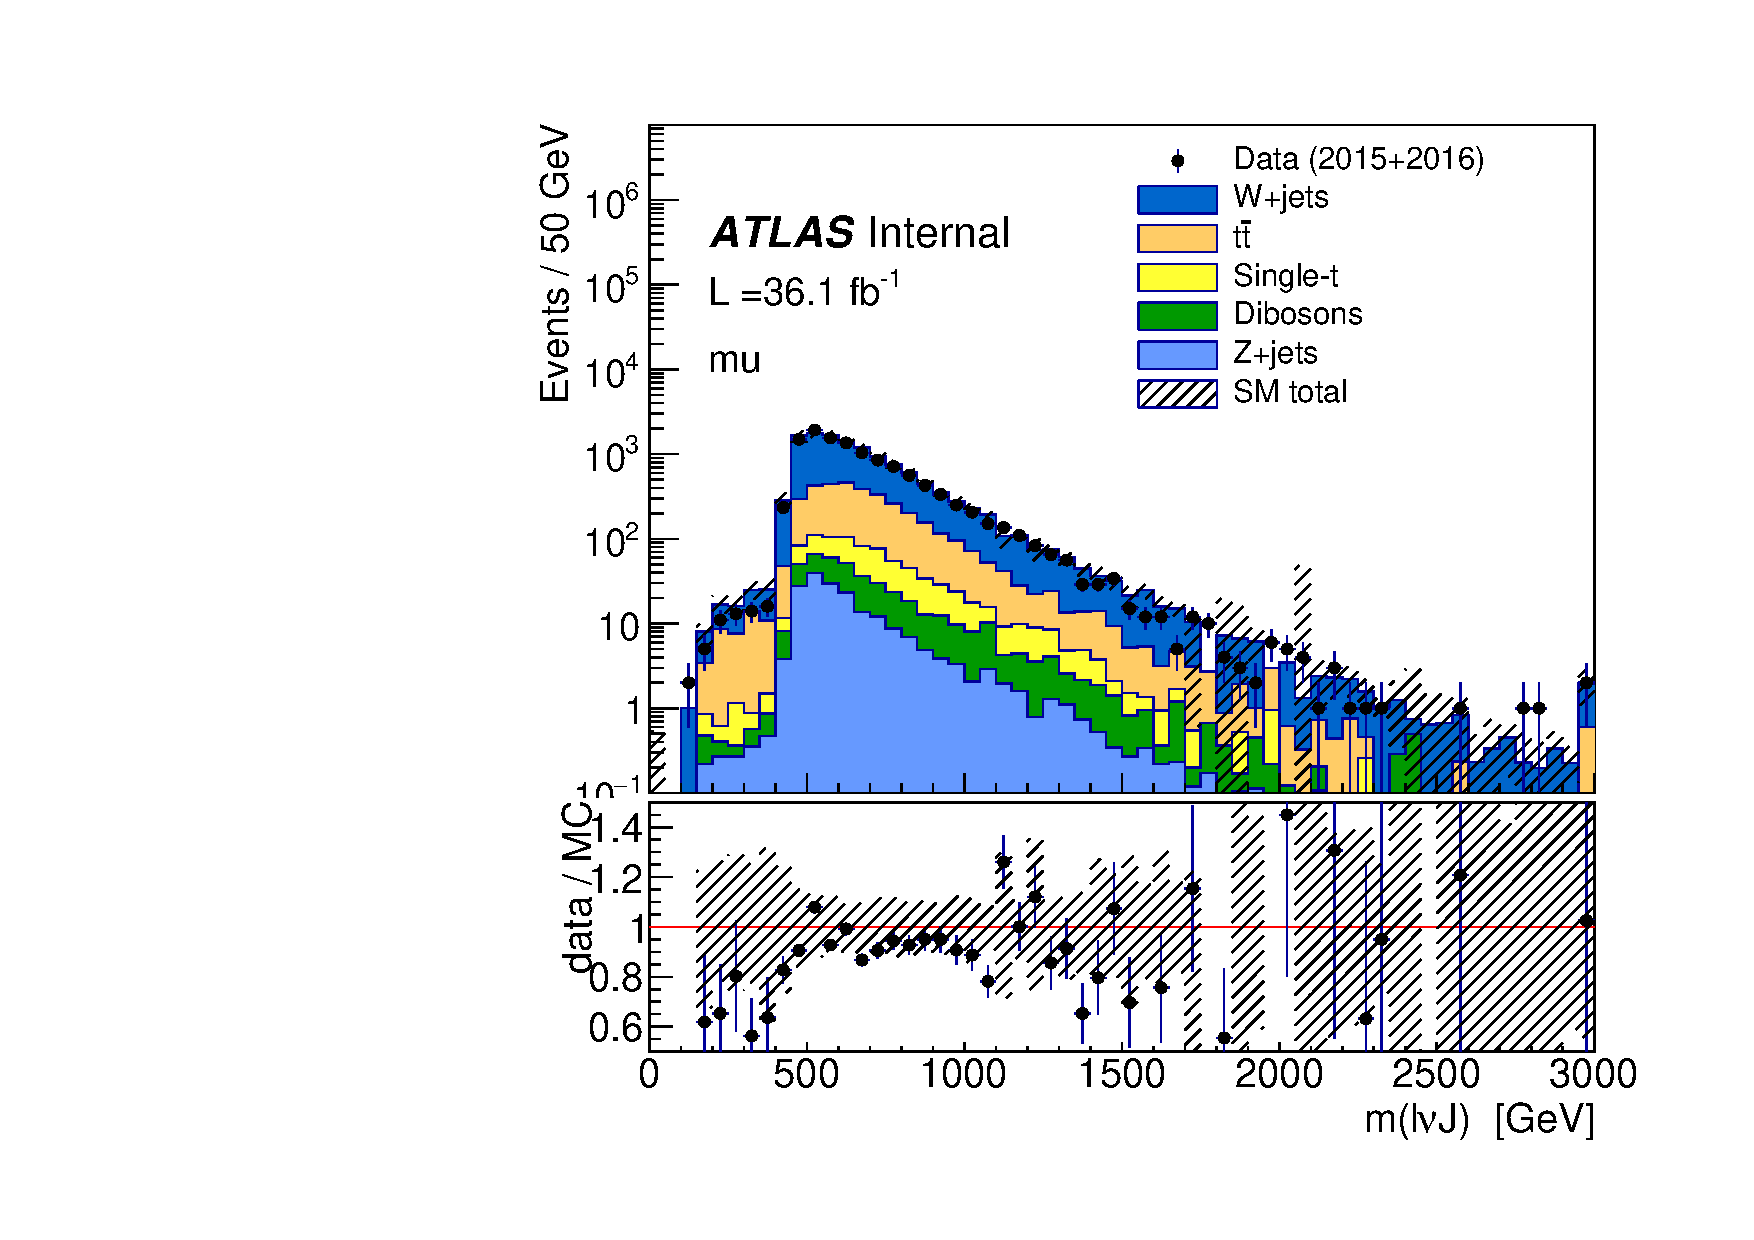
\includegraphics[width=0.43\textwidth]{Chapter3/LowPurityCR_36fb/VVM_12_mu}}\\
    \subfloat[]{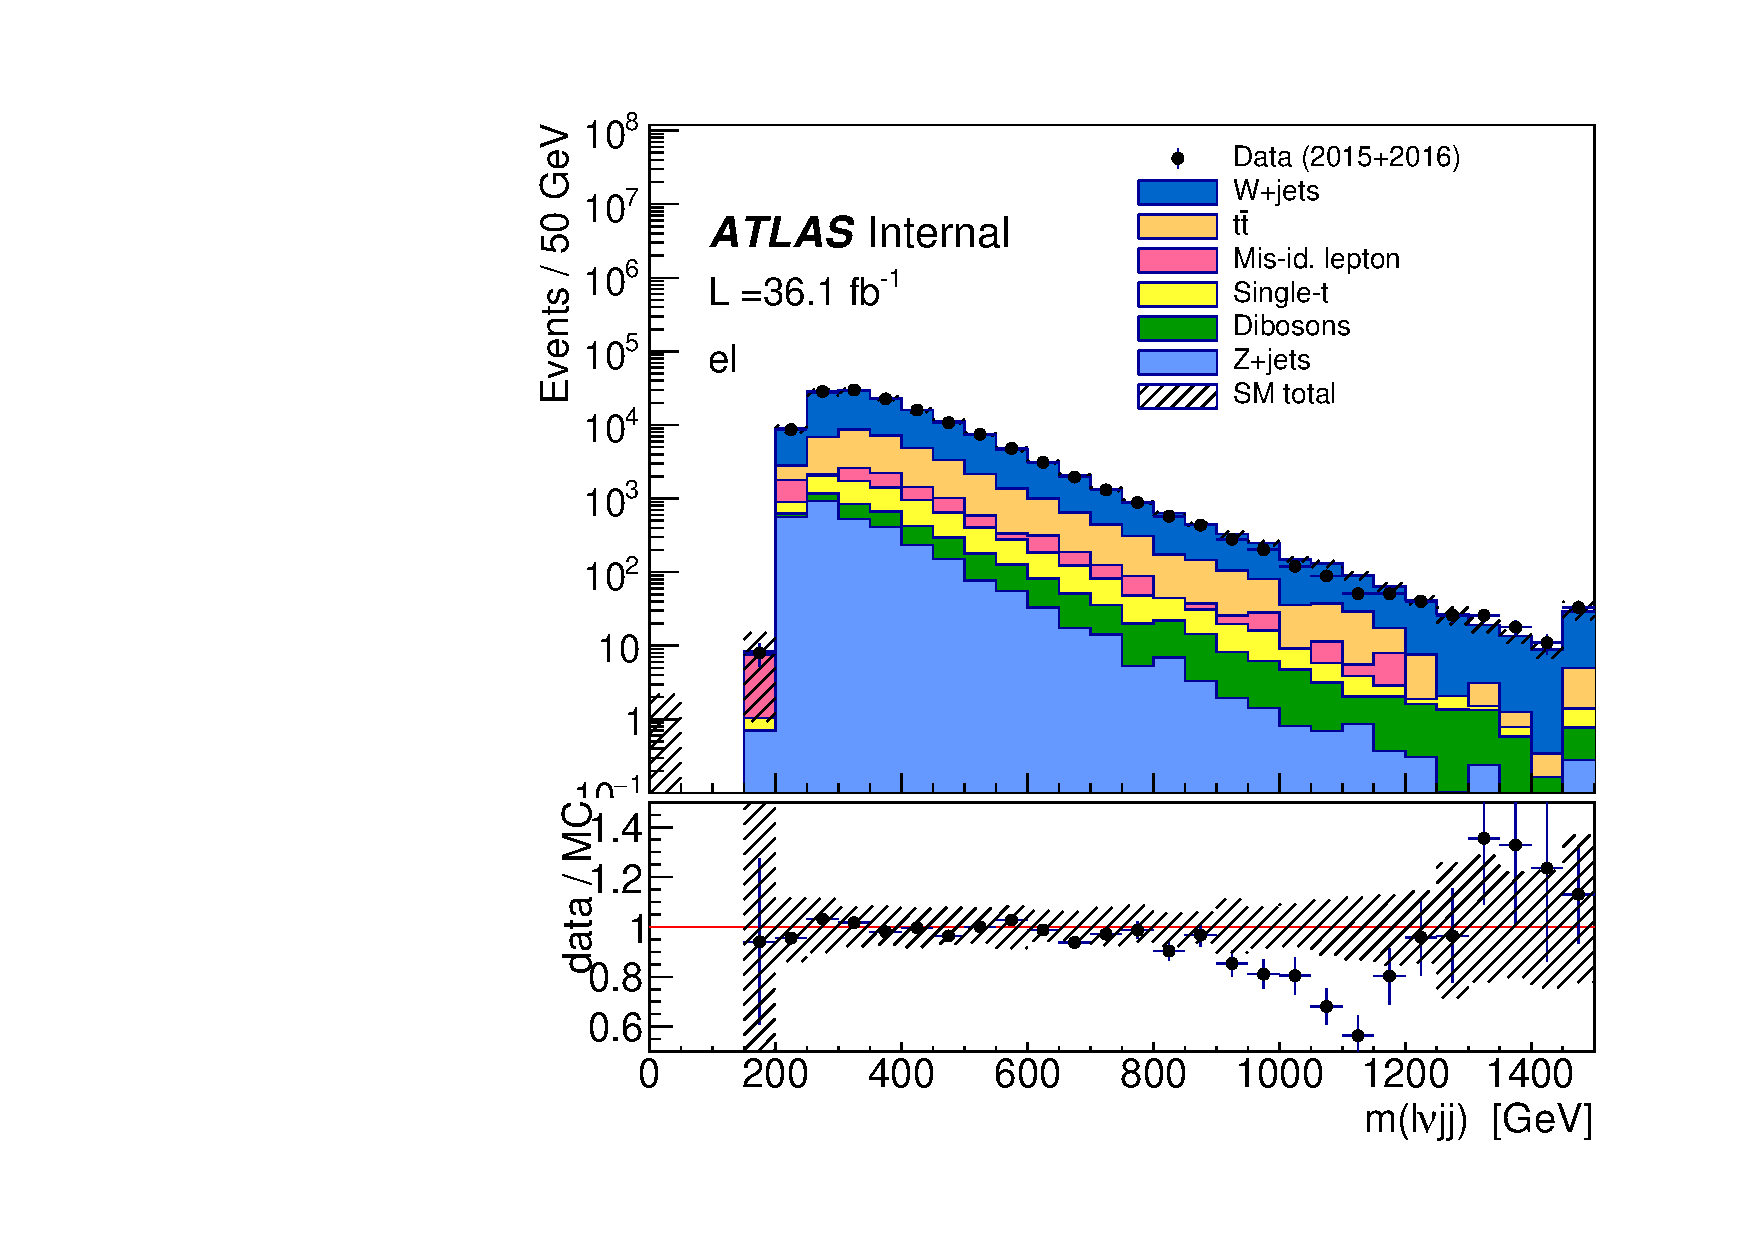
\includegraphics[width=0.43\textwidth]{Chapter3/ResolvedCR/ggF36fb/VVM_5_el}}
	\subfloat[]{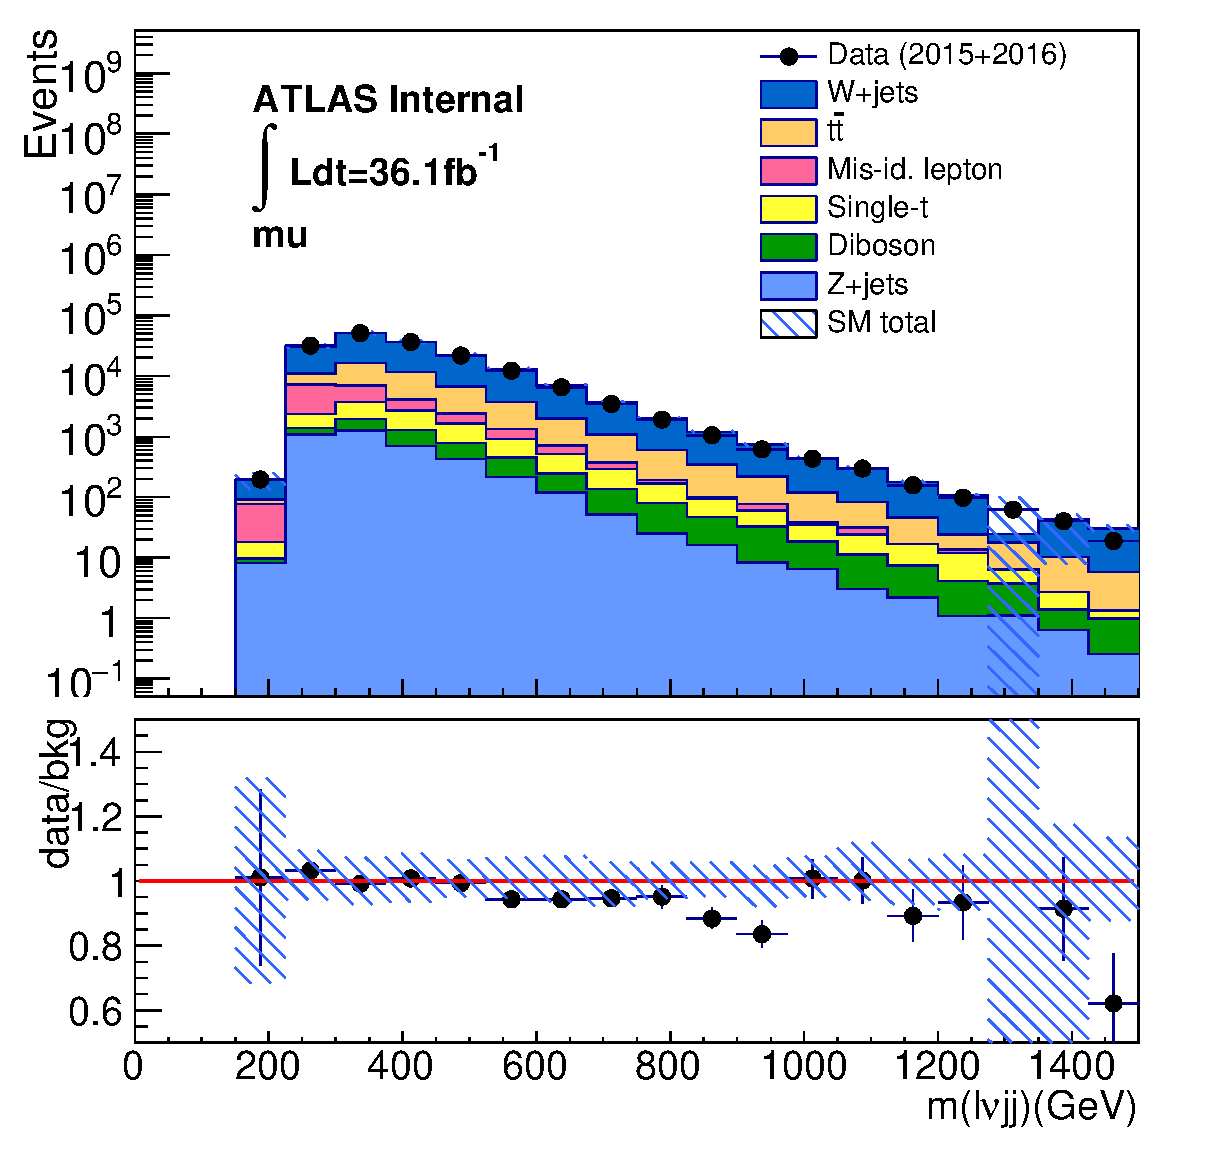
\includegraphics[width=0.43\textwidth]{Chapter3/ResolvedCR/ggF36fb/VVM_5_mu.eps}}
	\caption{The distribution of $m_{WV}$ in ggF high purity (top), low purity (middle), and resolved (bottom) W+jet control region for electron (left) and muon (right) channels respectively}
	\label{Fig:ggFWR}
\end{figure}



\begin{figure}[ht]
	\centering
	\subfloat[]{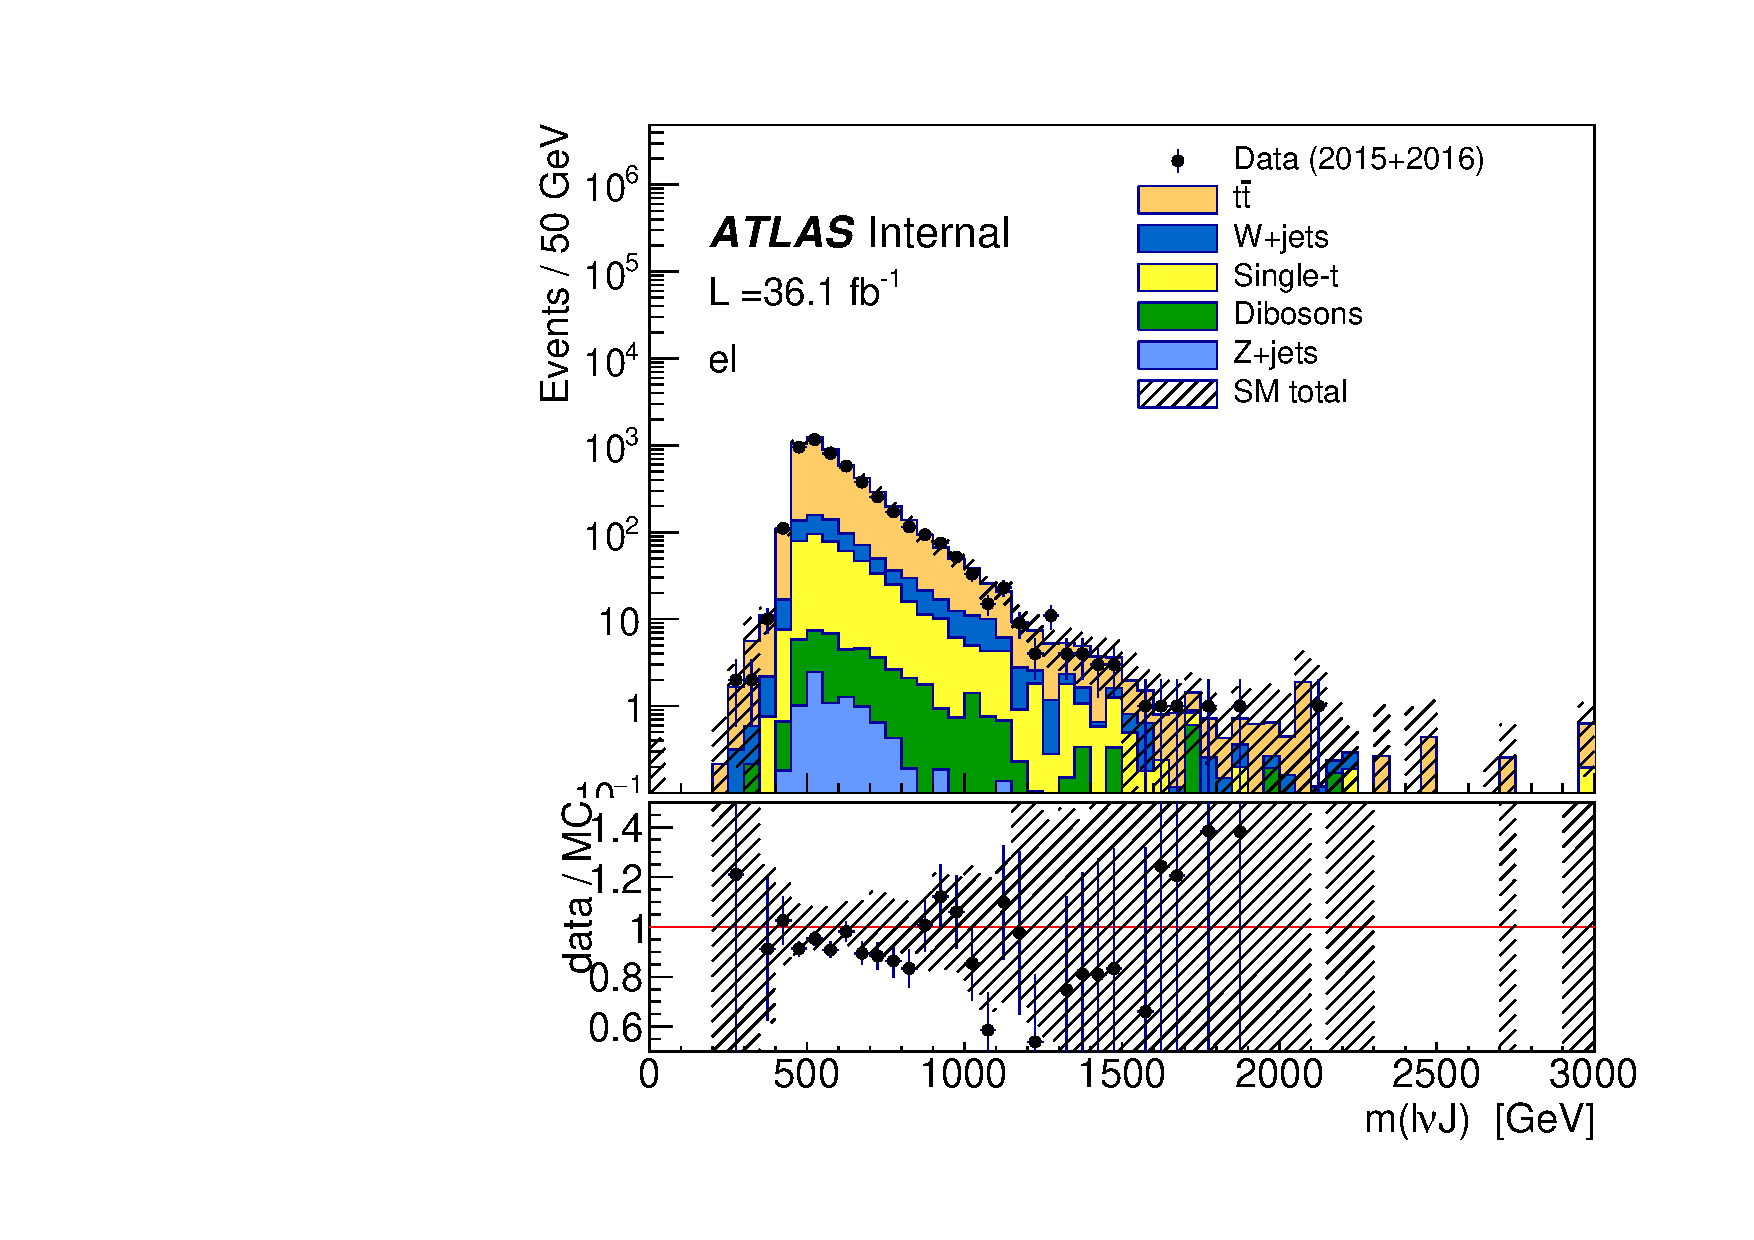
\includegraphics[width=0.43\textwidth]{Chapter3/HighPurityCR_36fb/VVM_2_el}}
	\subfloat[]{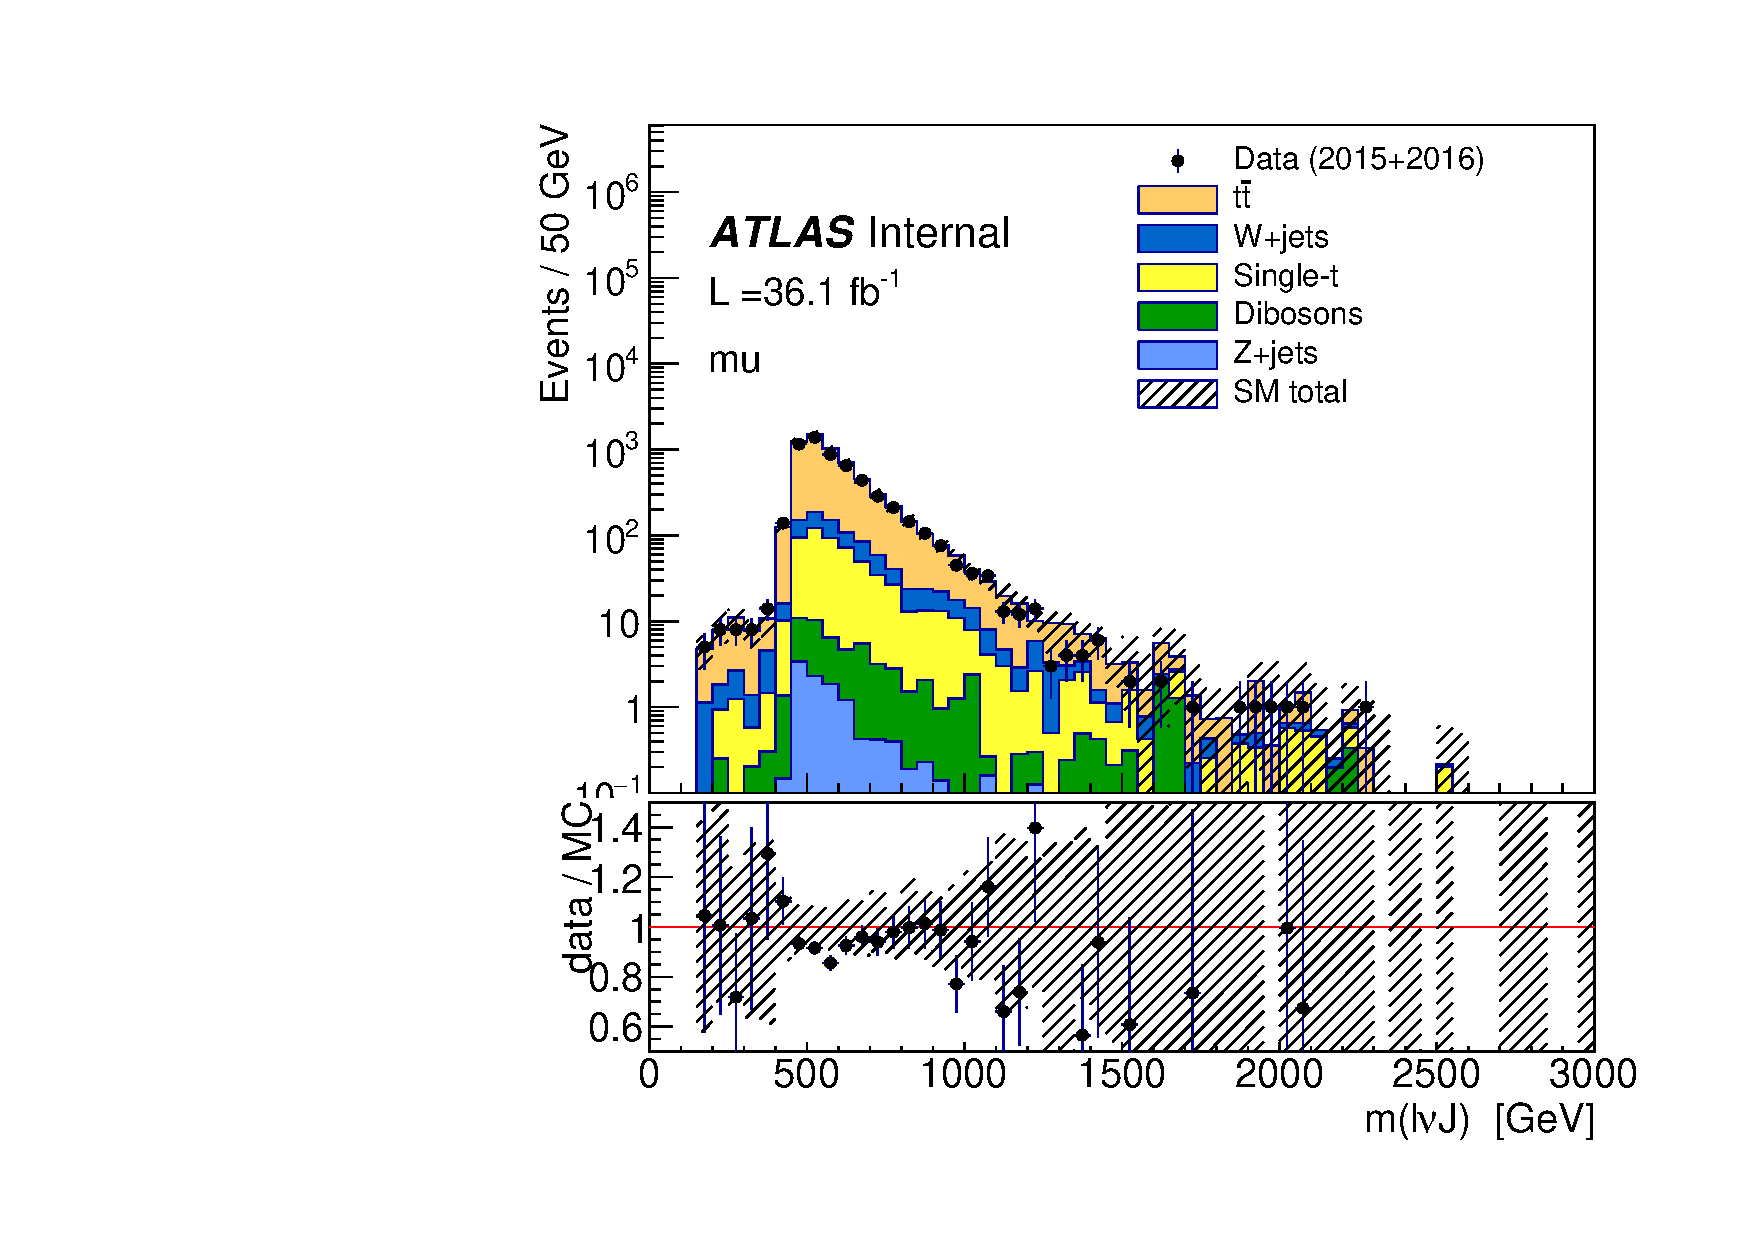
\includegraphics[width=0.43\textwidth]{Chapter3/HighPurityCR_36fb/VVM_2_mu}}\\
	\subfloat[]{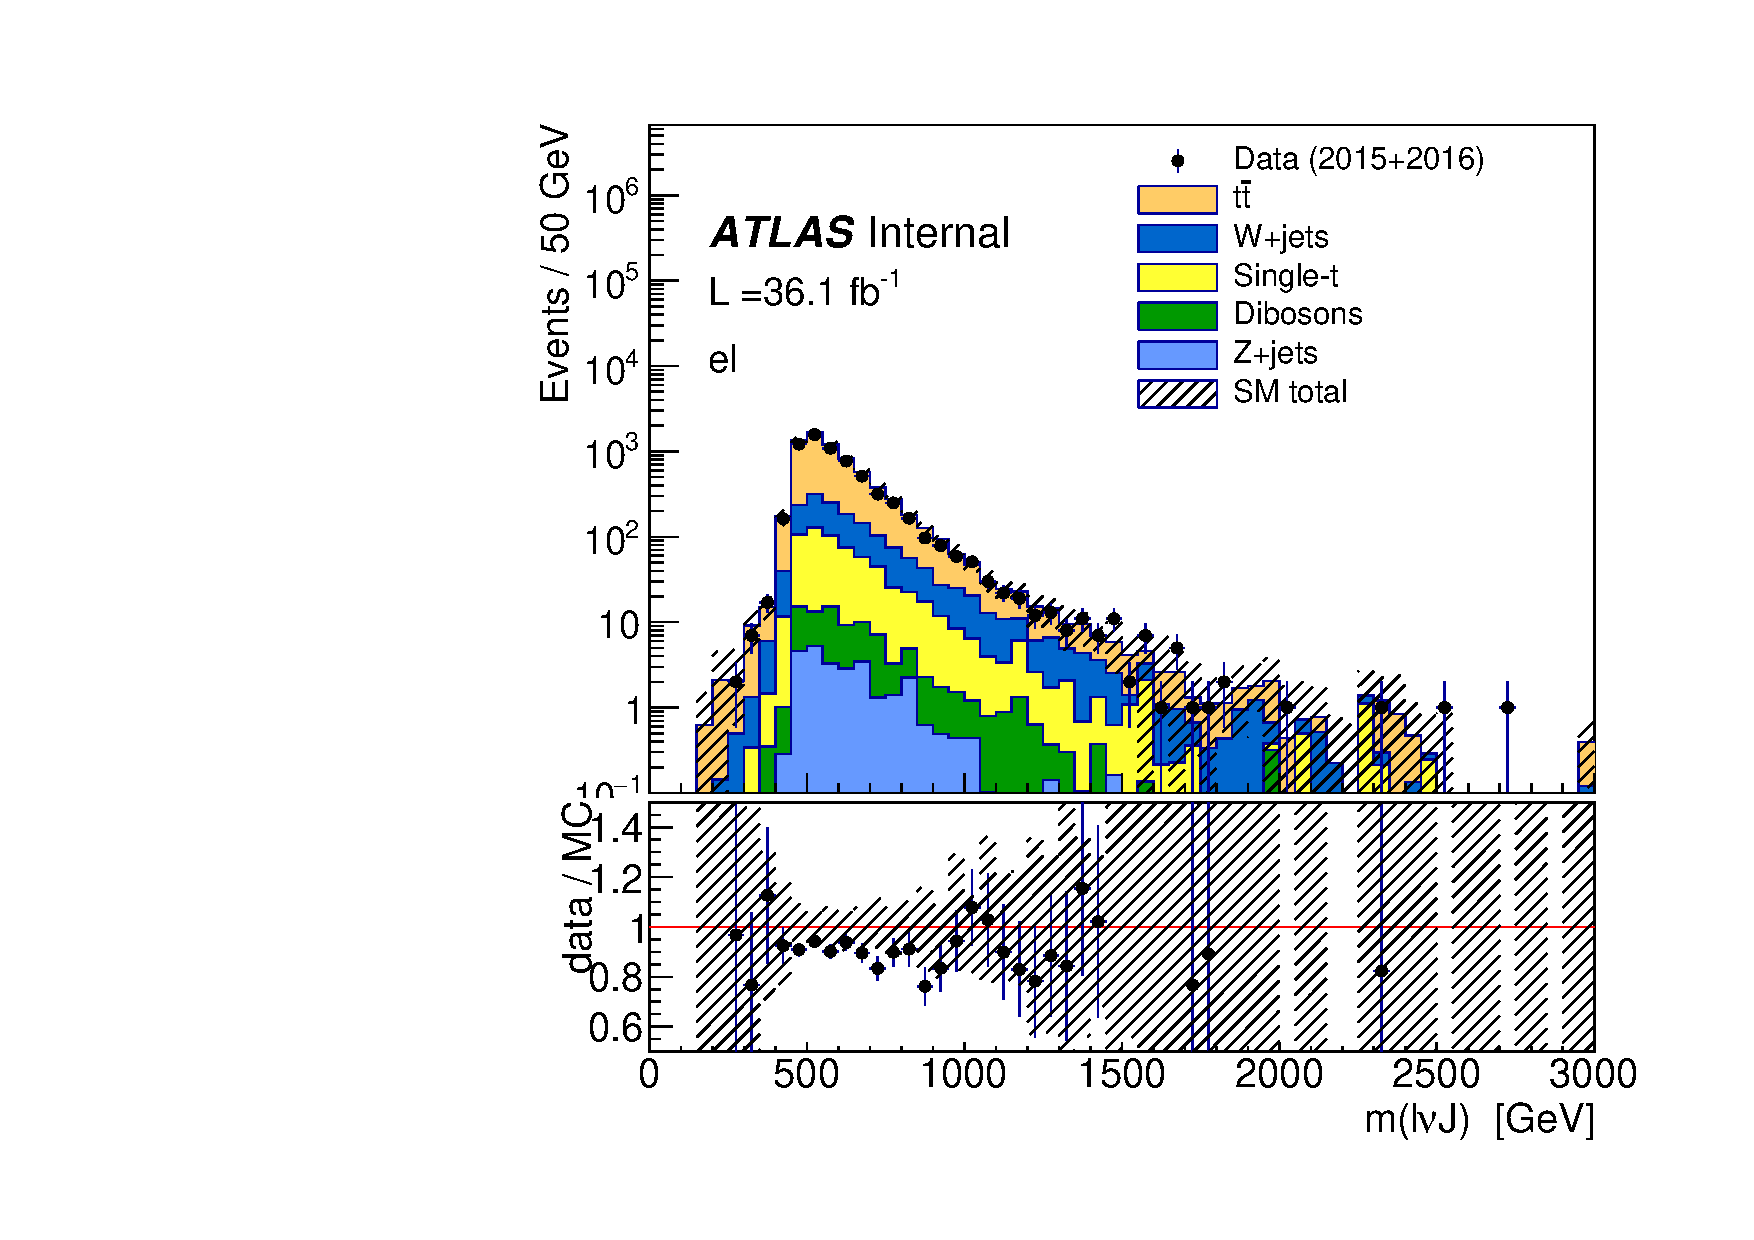
\includegraphics[width=0.43\textwidth]{Chapter3/LowPurityCR_36fb/VVM_13_el}}
    \subfloat[]{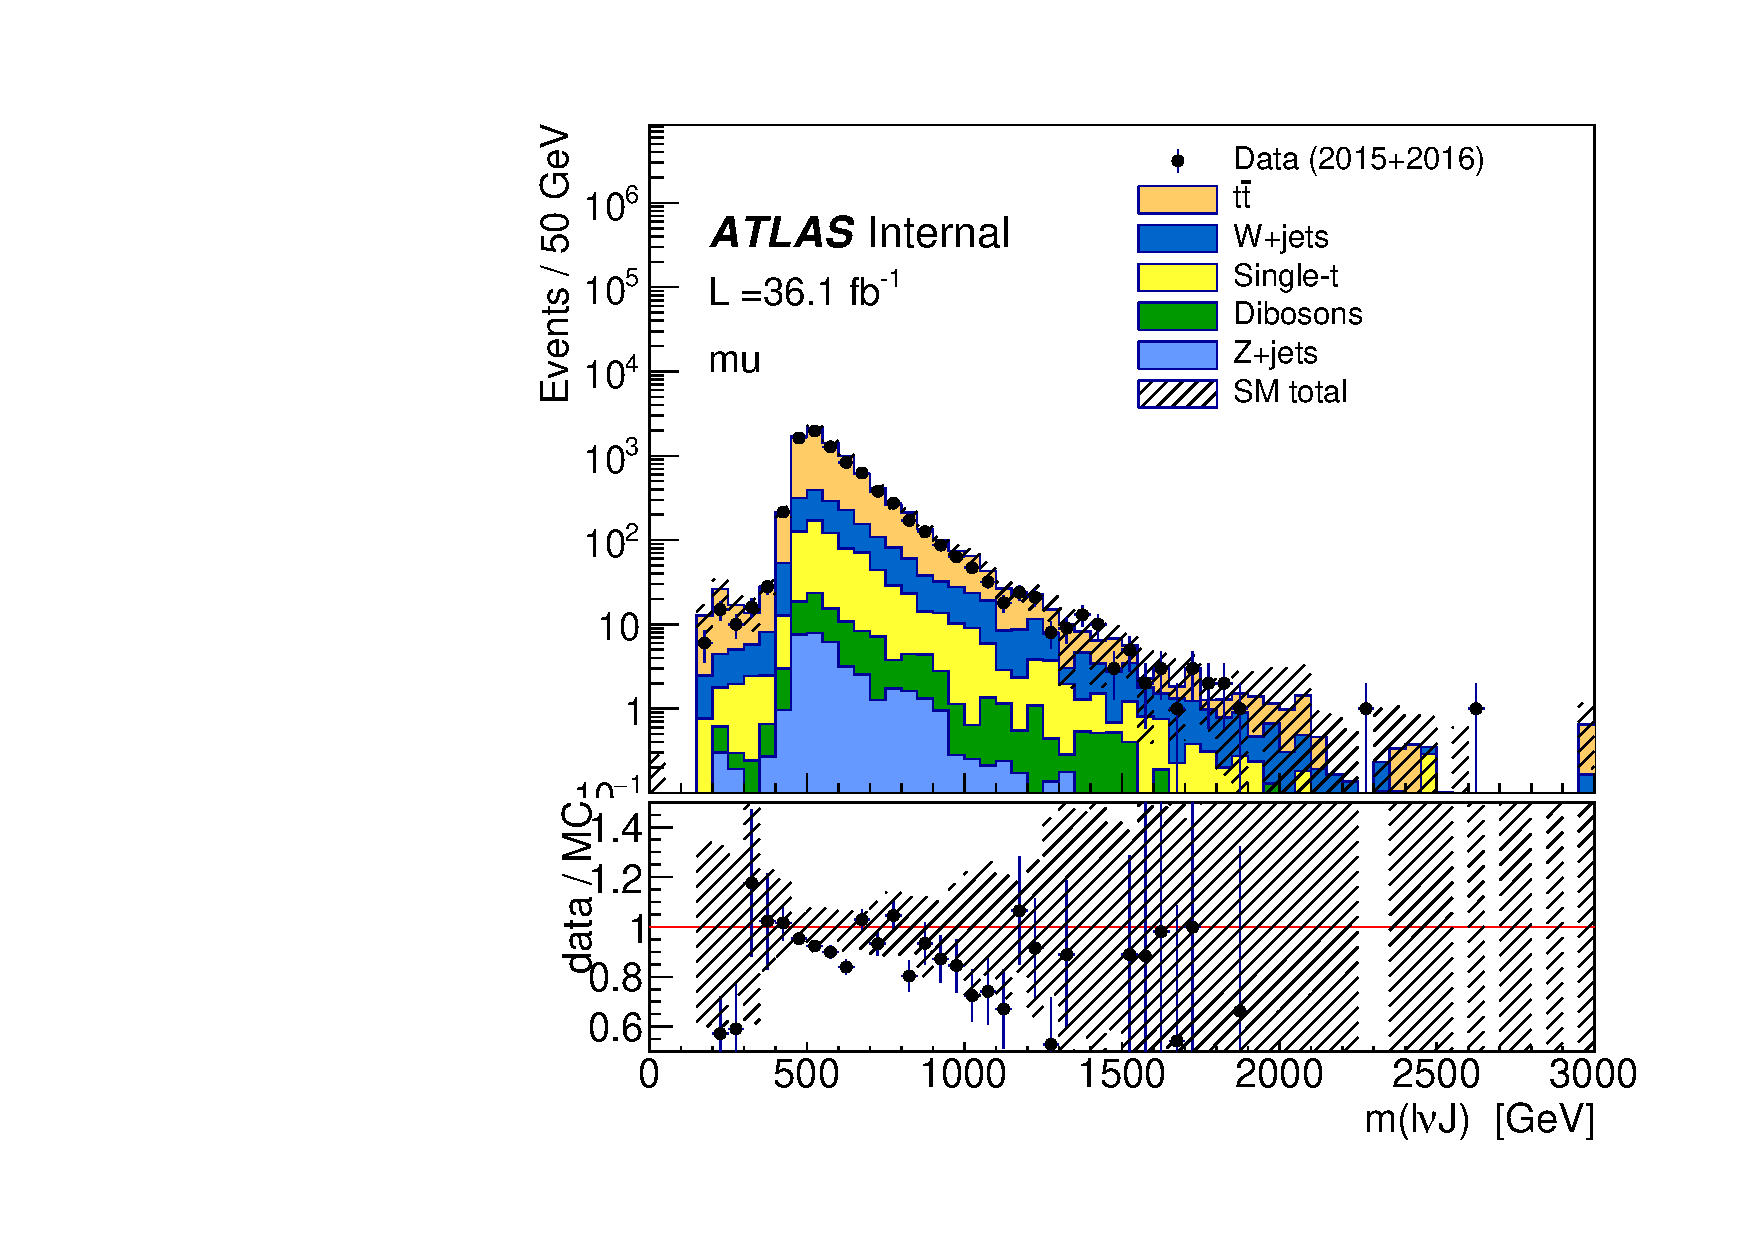
\includegraphics[width=0.43\textwidth]{Chapter3/LowPurityCR_36fb/VVM_13_mu}}\\
	\subfloat[]{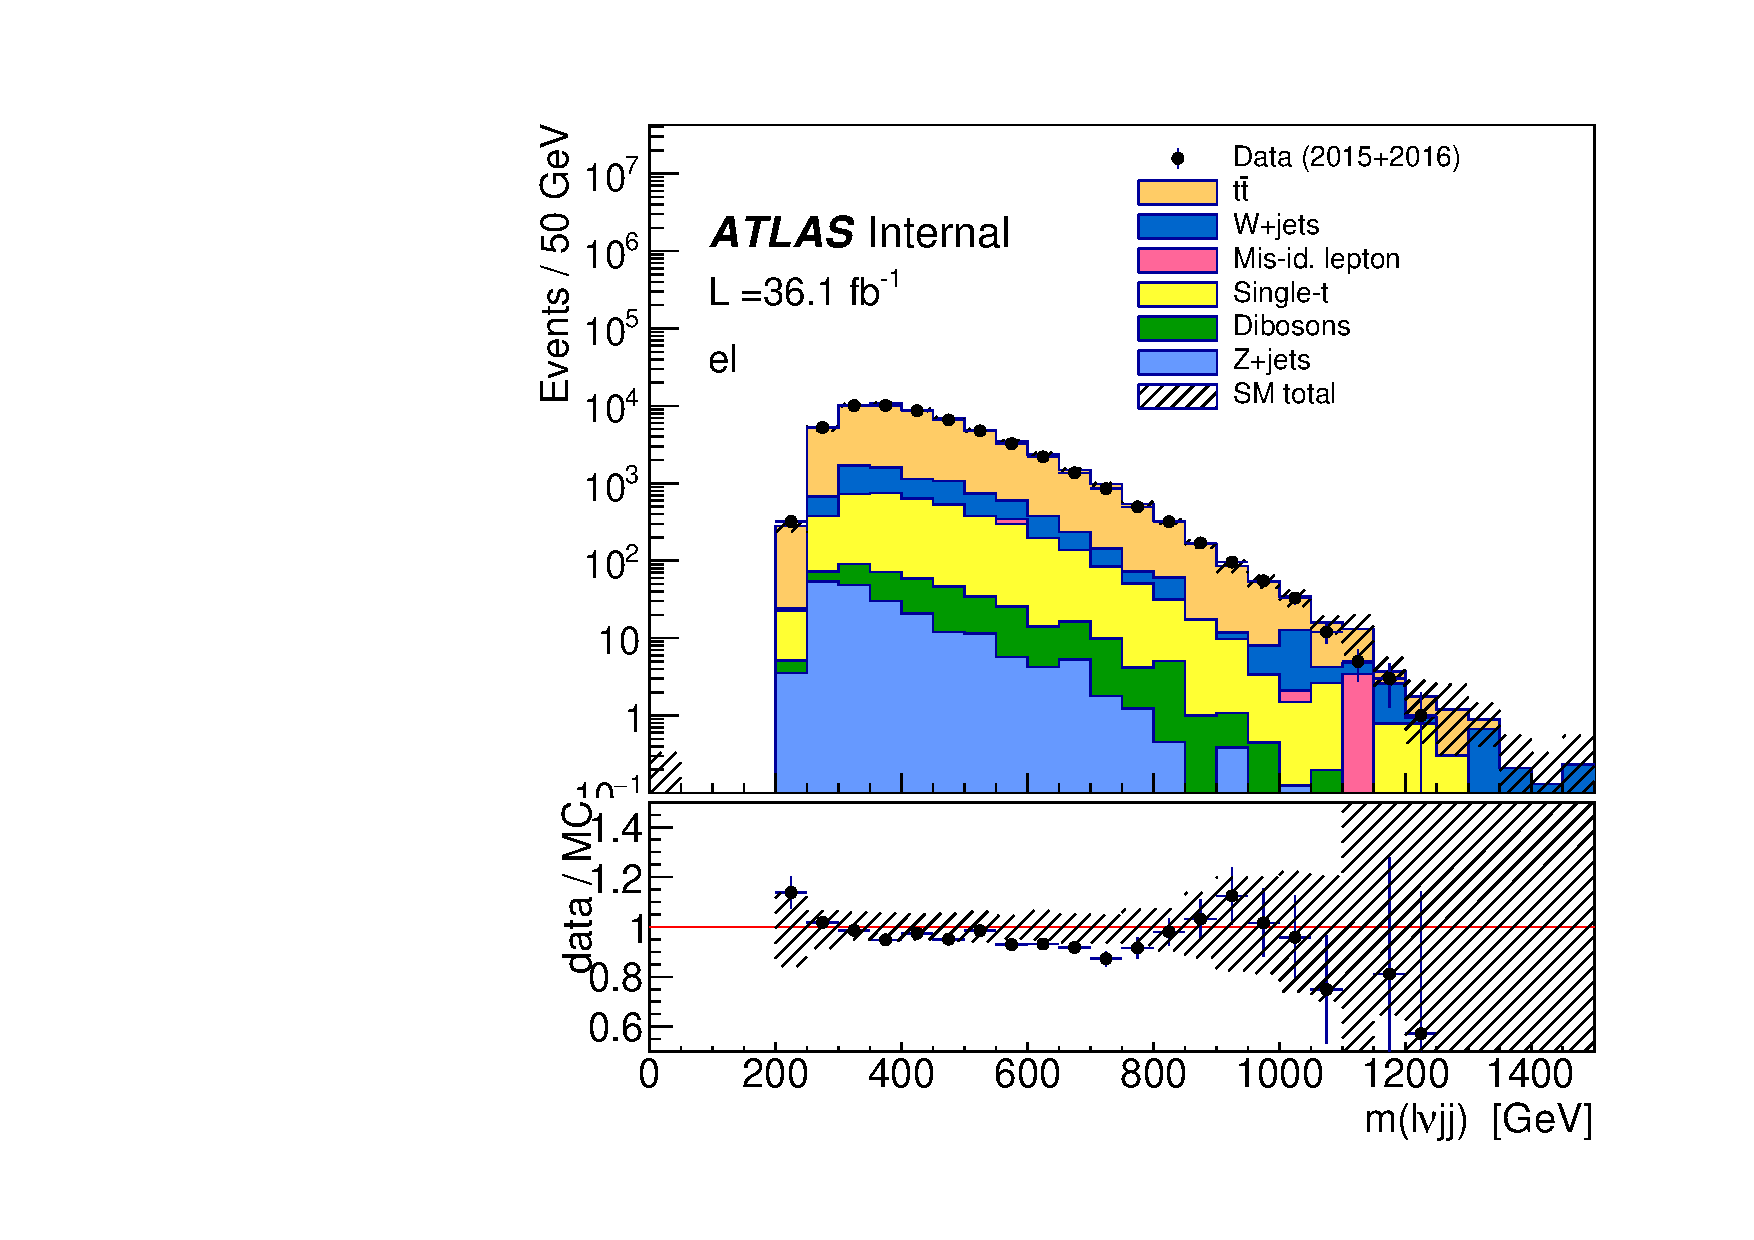
\includegraphics[width=0.43\textwidth]{Chapter3/ResolvedCR/ggF36fb/VVM_6_el}}
    \subfloat[]{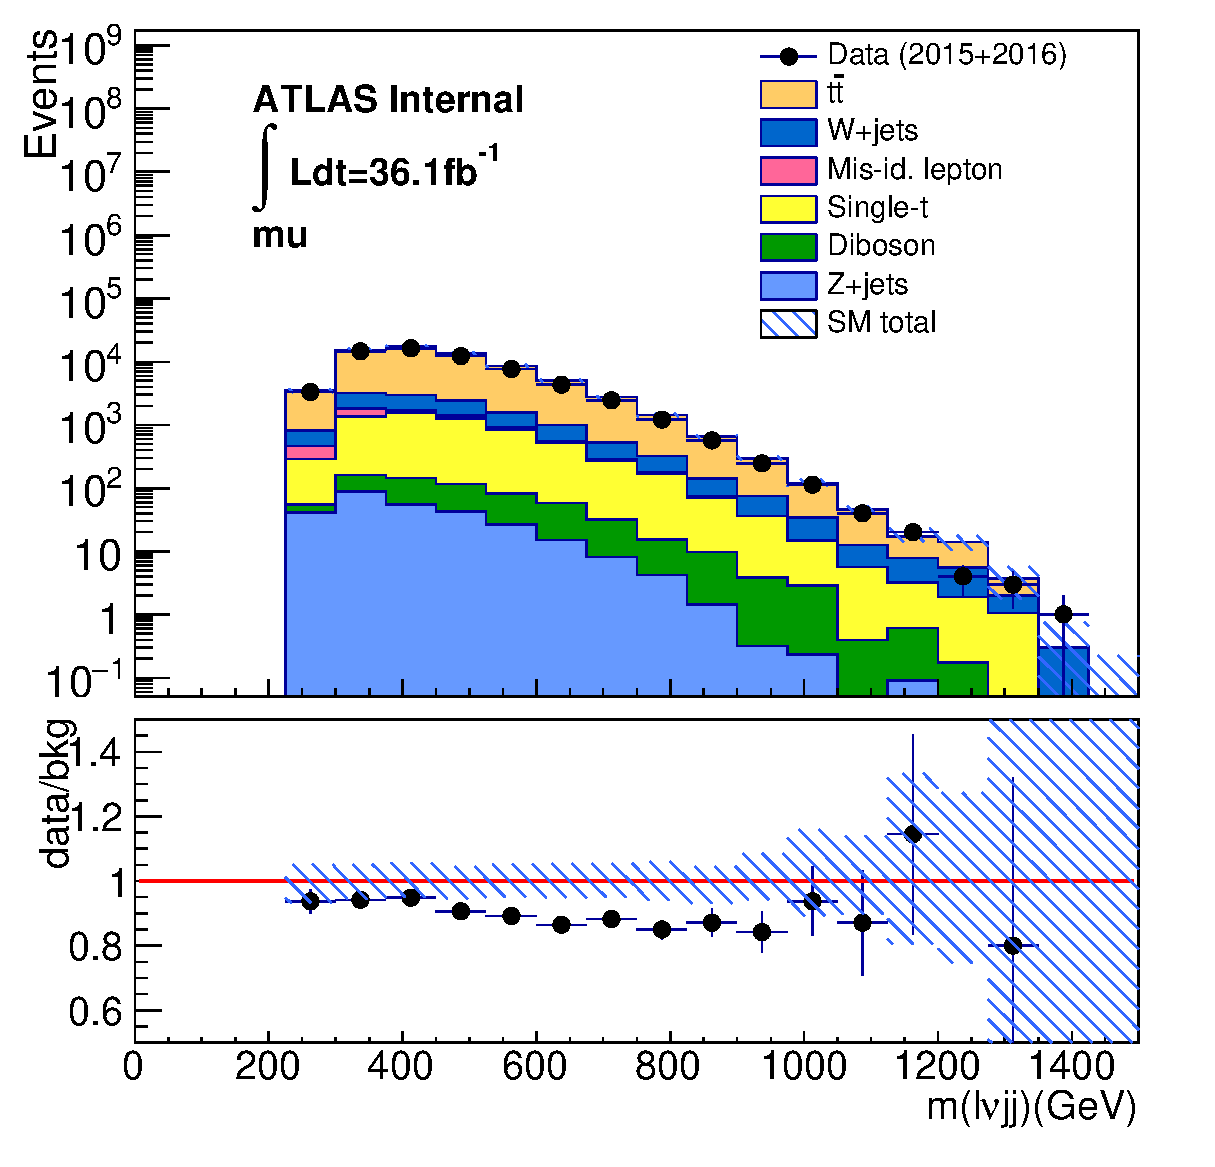
\includegraphics[width=0.43\textwidth]{Chapter3/ResolvedCR/ggF36fb/VVM_6_mu.eps}}
	\caption{The distribution of $m_{WV}$ in ggF high purity (top), low purity (middle), and resolved (bottom) top control region for electron (left) and muon (right) channels respectively}
	 \label{Fig:ggFTR}
\end{figure}


\begin{figure}[ht]
	\centering
	\subfloat[]{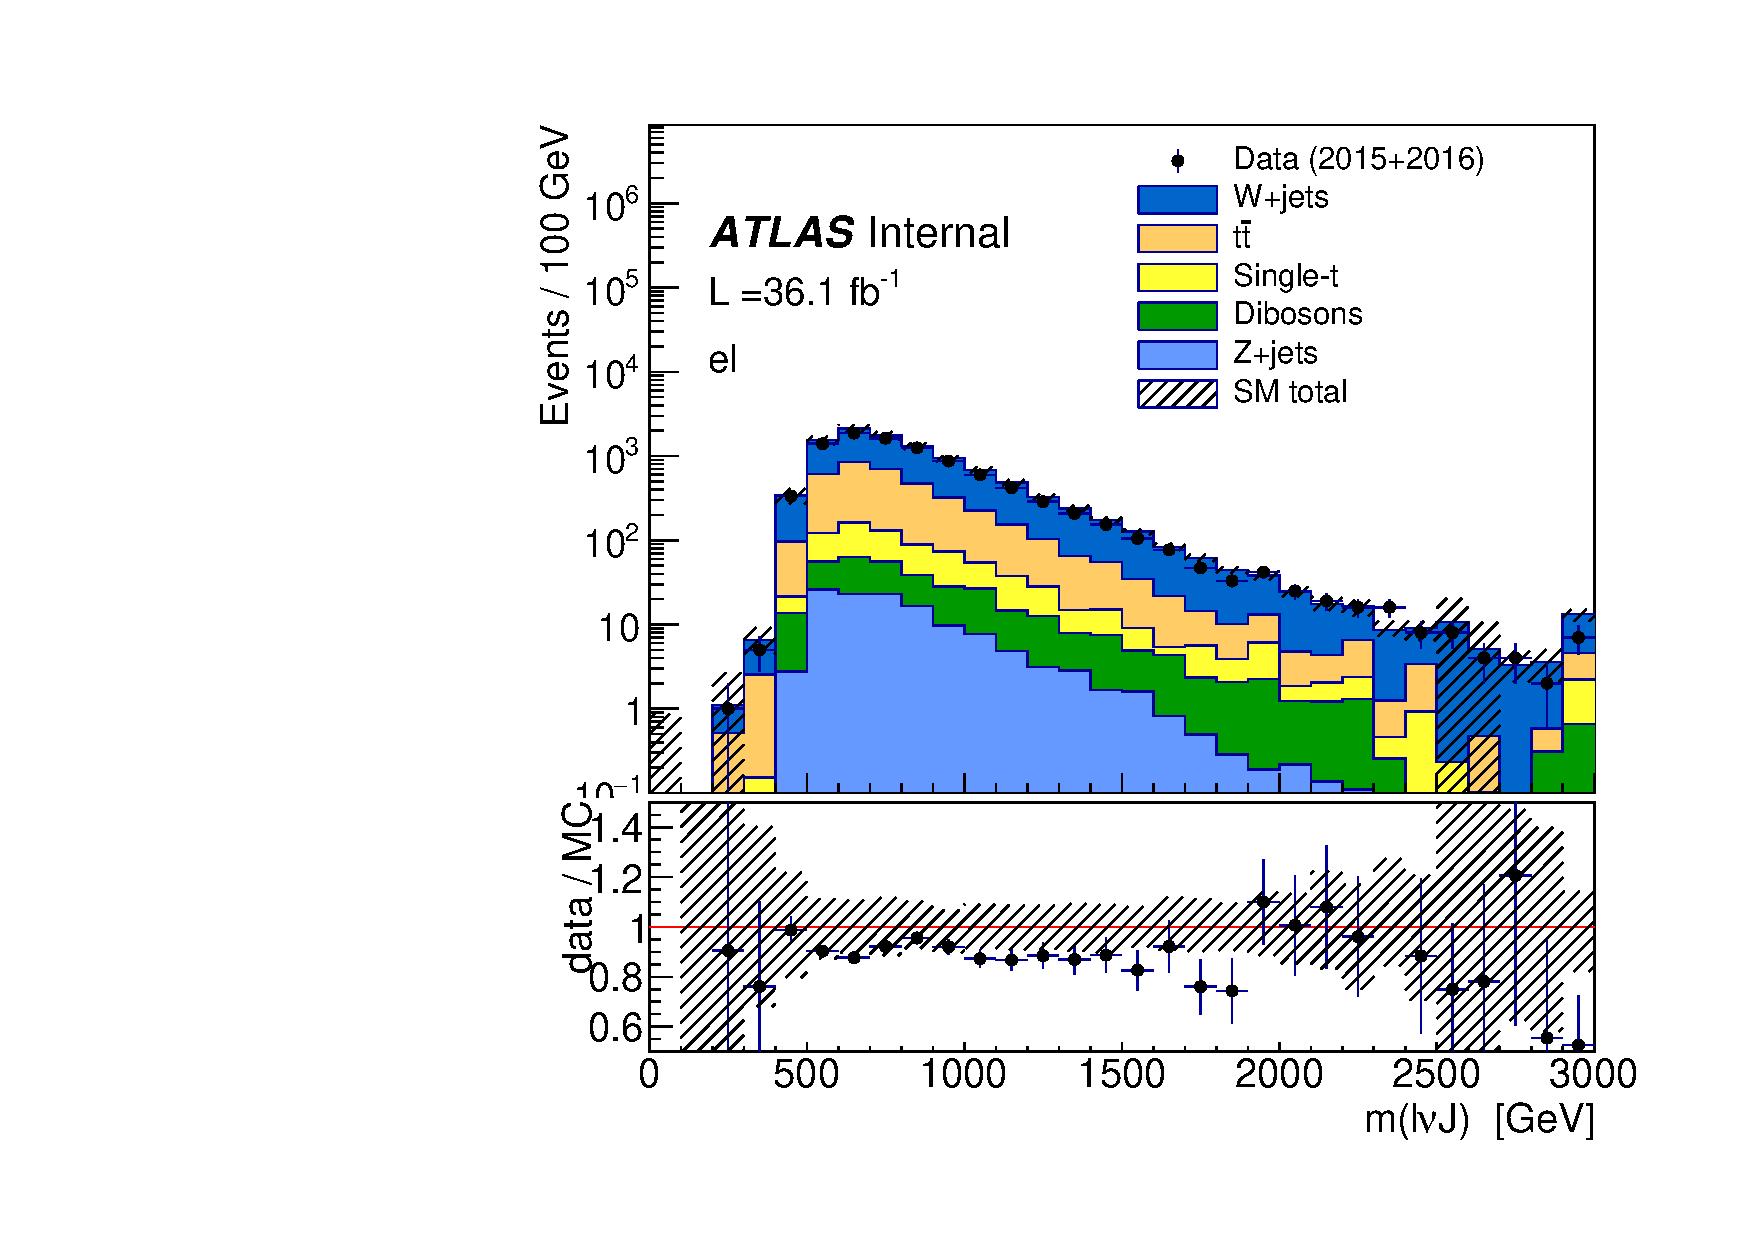
\includegraphics[width=0.43\textwidth]{Chapter3/VBF36fbHP/VVM_3_el}}
	\subfloat[]{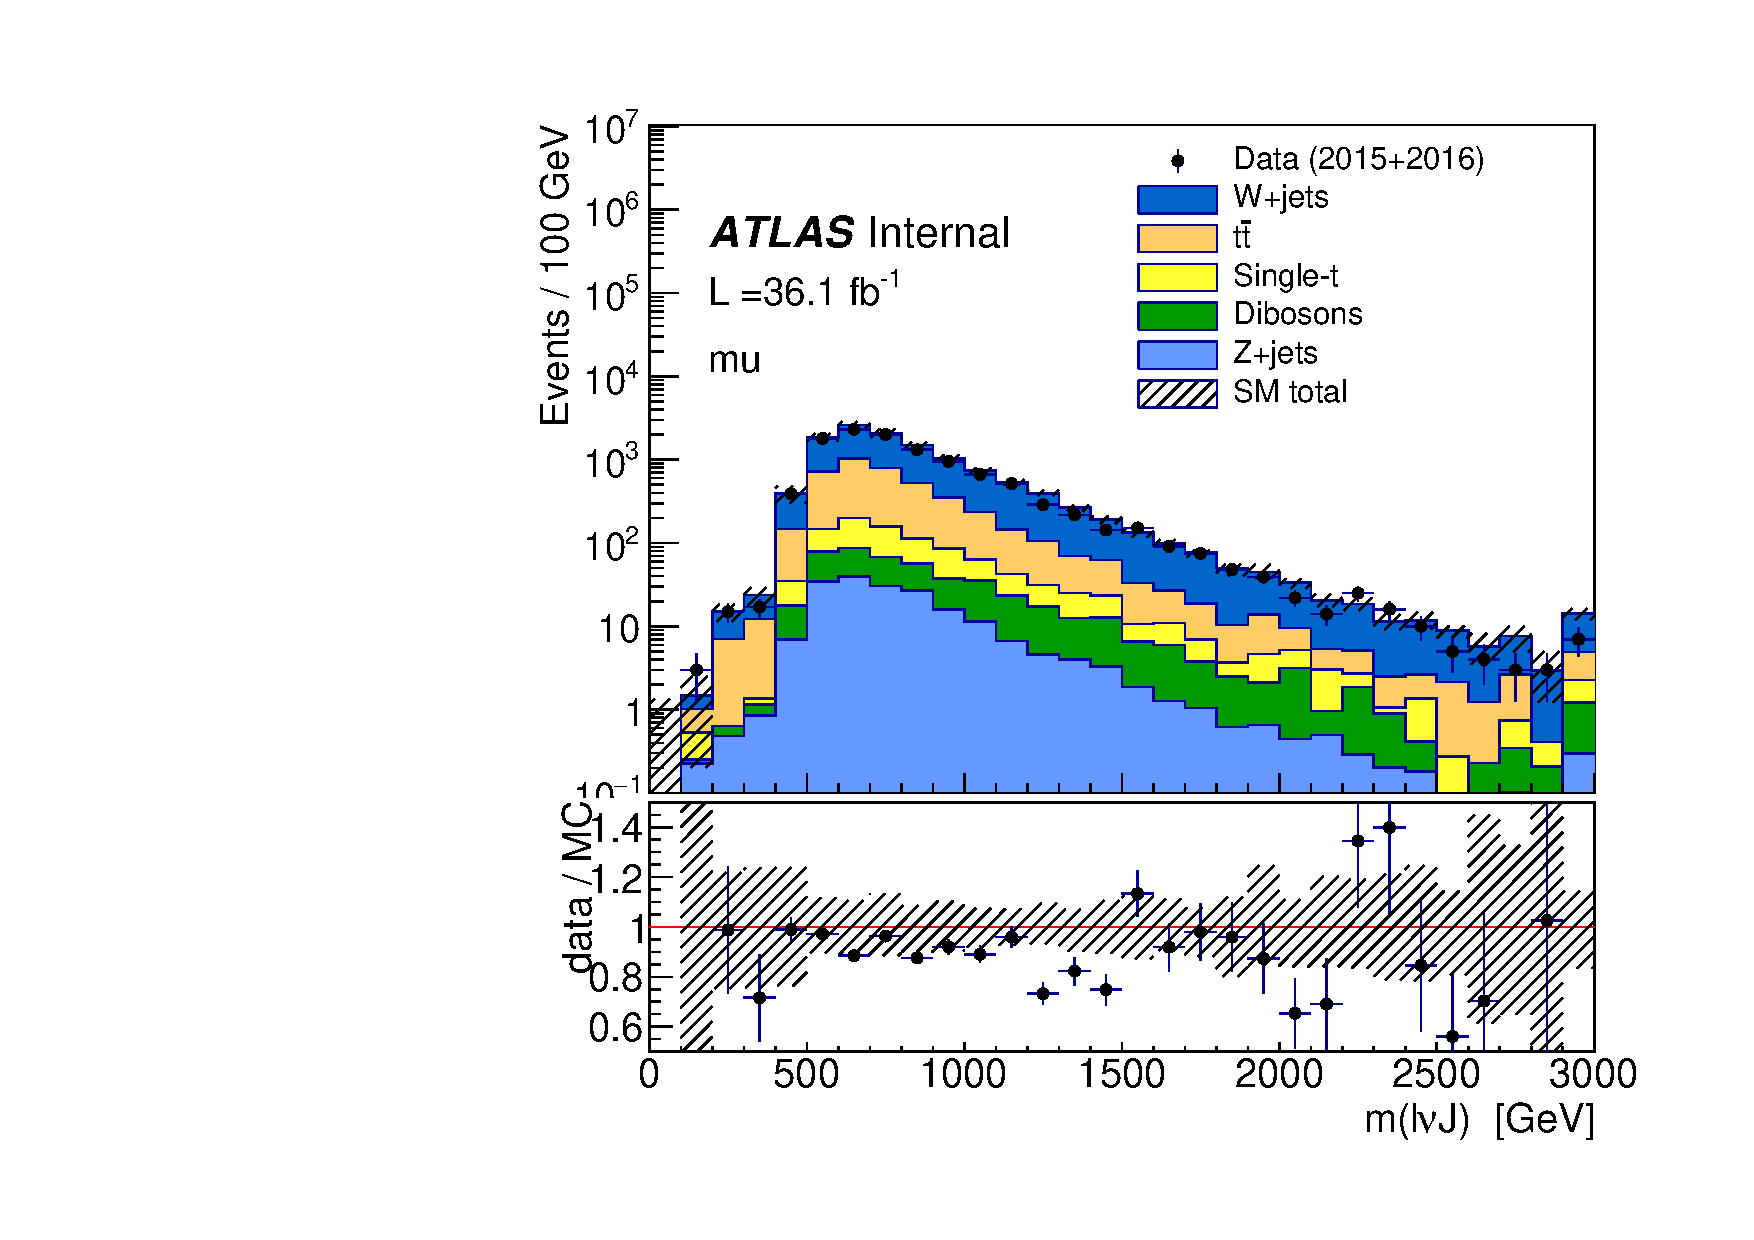
\includegraphics[width=0.43\textwidth]{Chapter3/VBF36fbHP/VVM_3_mu}}\\
	\subfloat[]{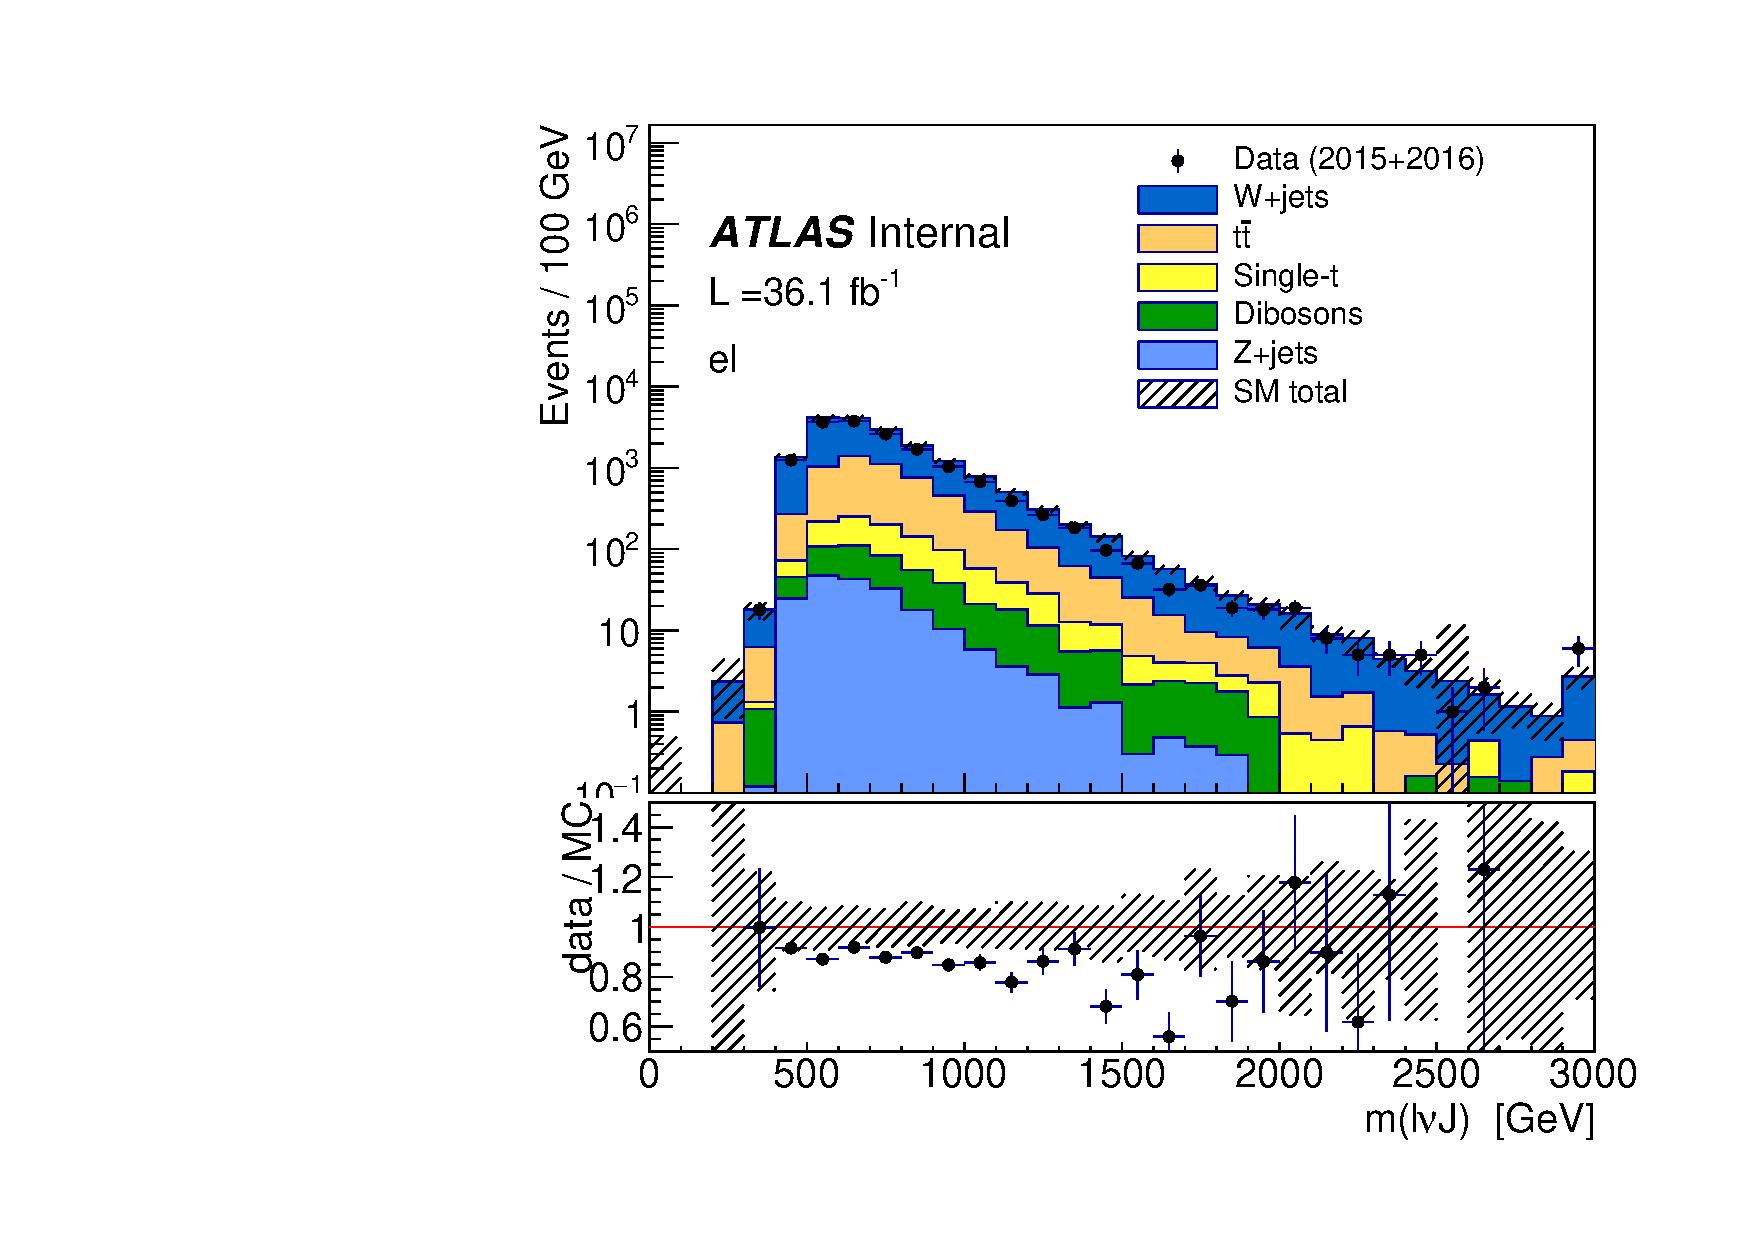
\includegraphics[width=0.43\textwidth]{Chapter3/VBF36fbLP/VVM_12_el}}
    \subfloat[]{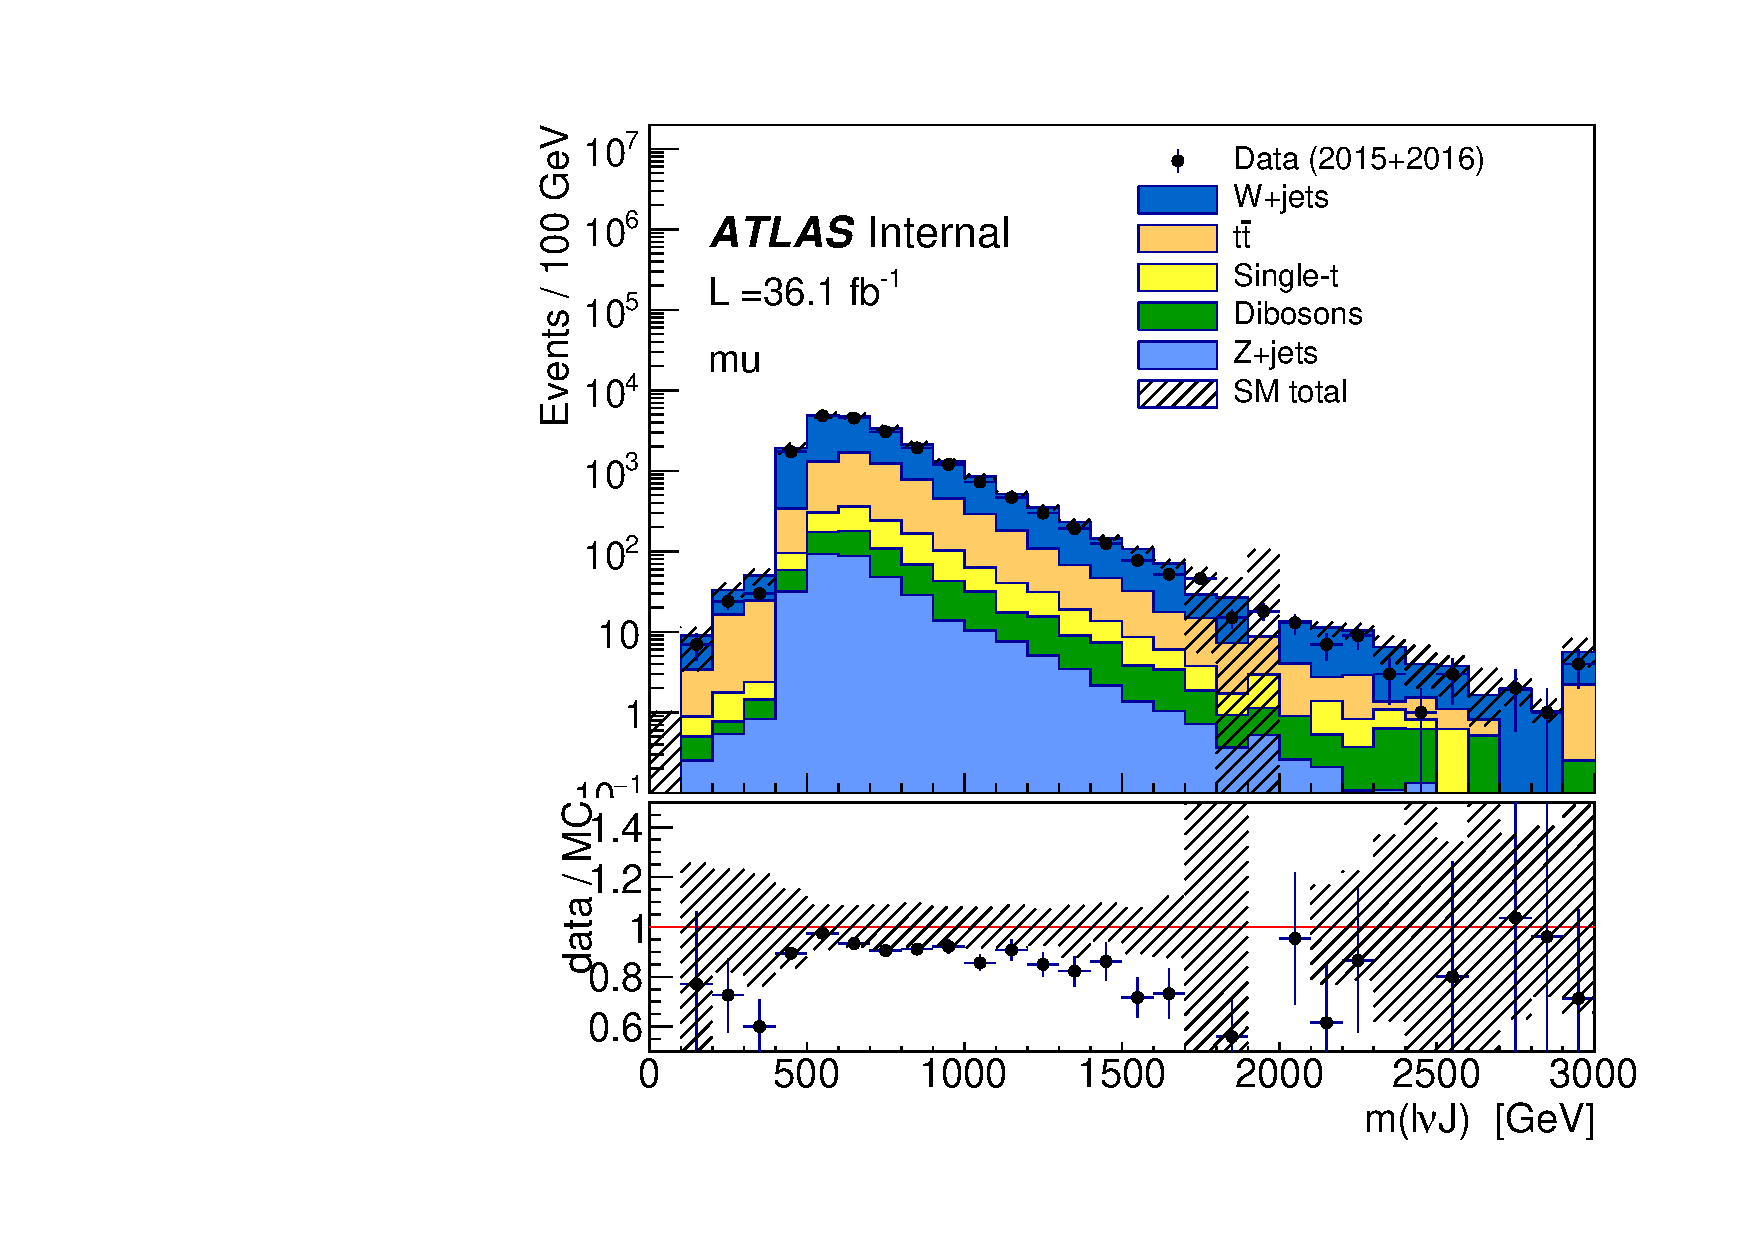
\includegraphics[width=0.43\textwidth]{Chapter3/VBF36fbLP/VVM_12_mu}}\\	
	\subfloat[]{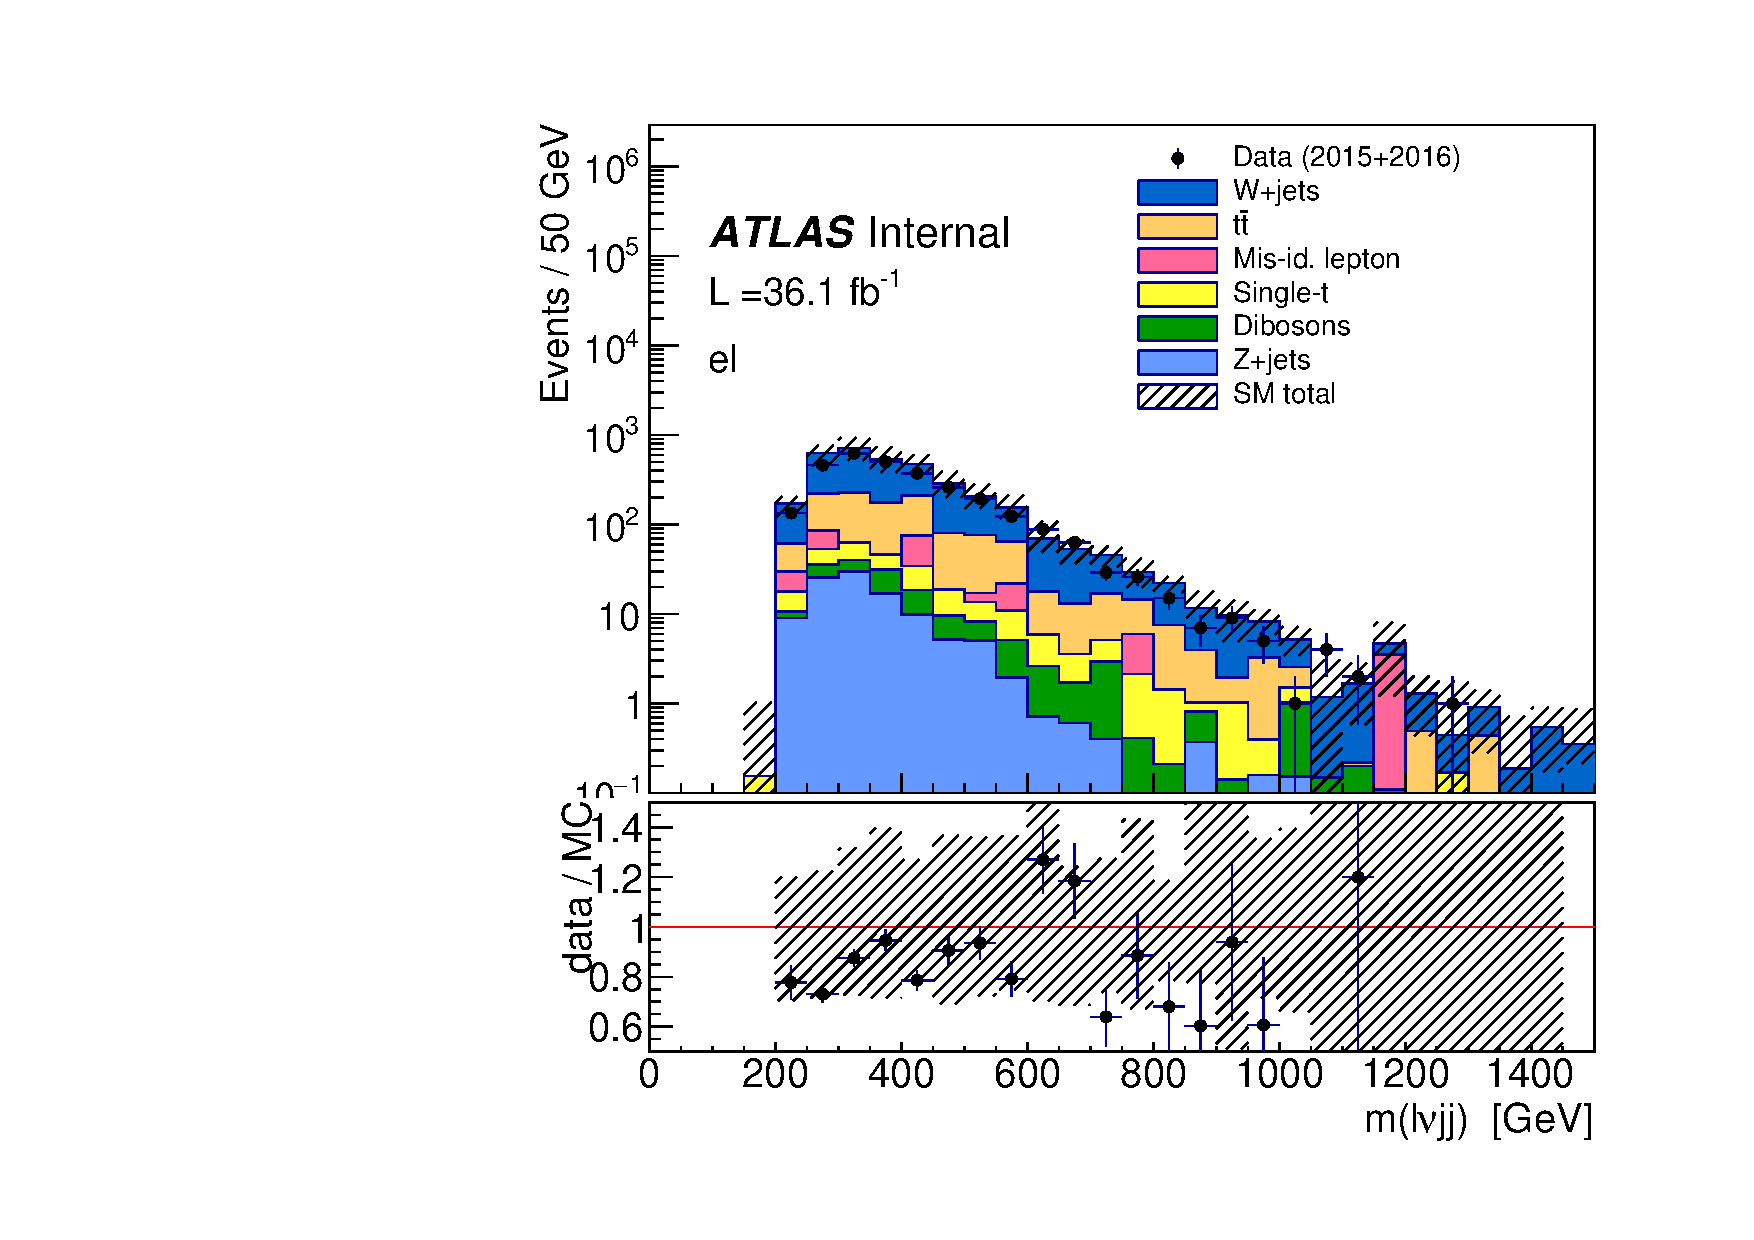
\includegraphics[width=0.43\textwidth]{Chapter3/ResolvedCR/VBF36fb/VVM_5_el}}
    \subfloat[]{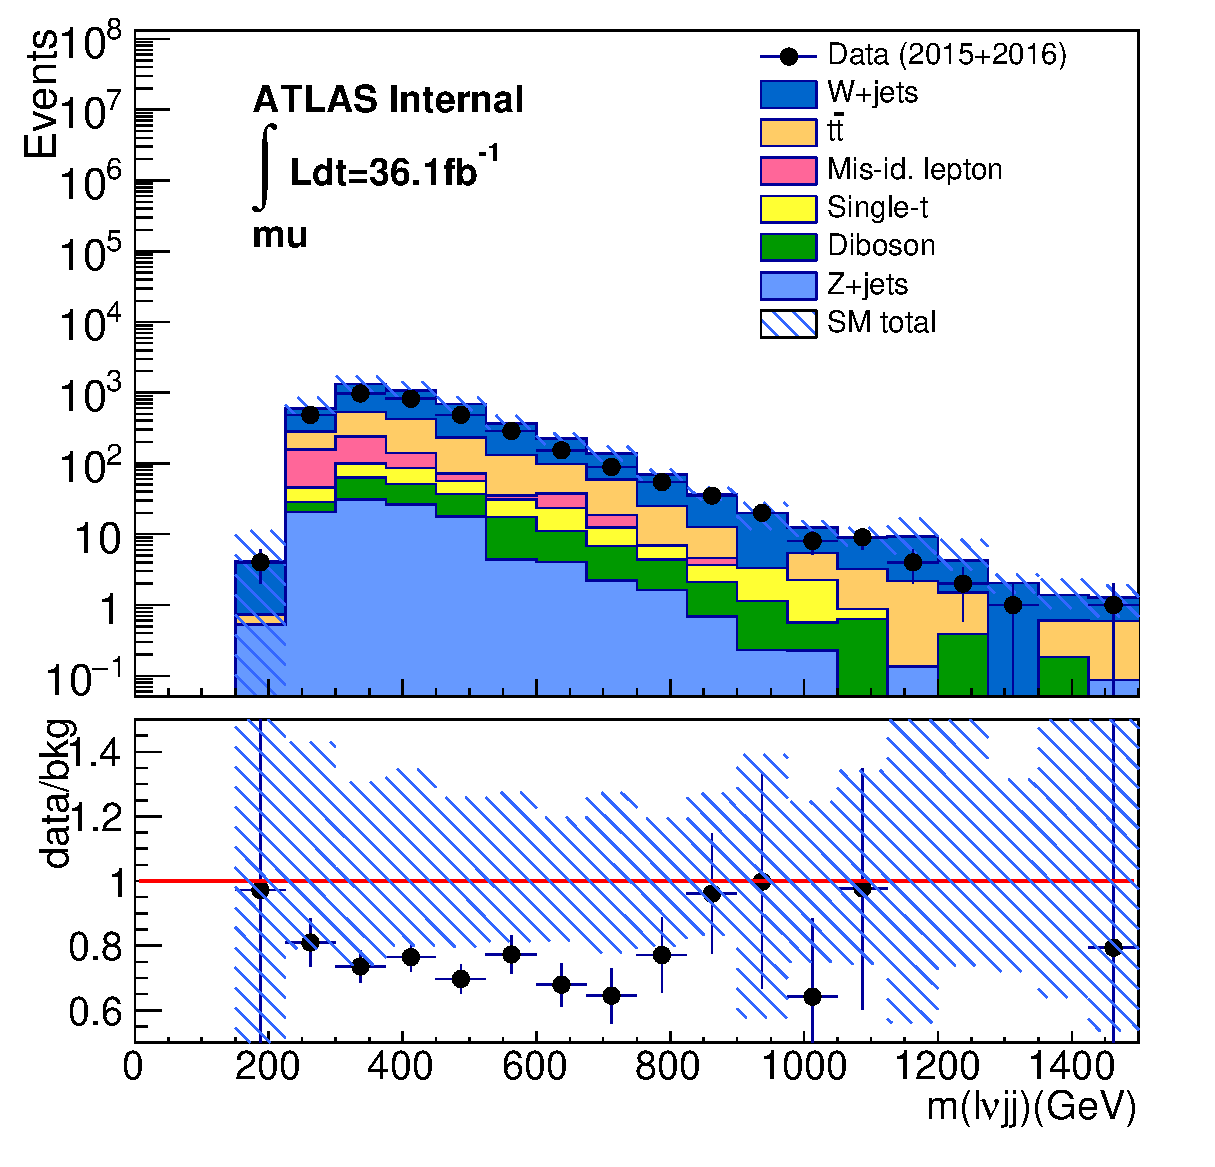
\includegraphics[width=0.43\textwidth]{Chapter3/ResolvedCR/VBF36fb/VVM_5_mu.eps}}    
	\caption{The distribution of $m_{WV}$ in VBF high purity (top), low purity (middle), and resolved (bottom) W+jet control region for electron (left) and muon (right) channels respectively}
	\label{Fig:mWVVBFWR}
\end{figure}
\clearpage
\begin{figure}[ht]
	\centering

	\subfloat[]{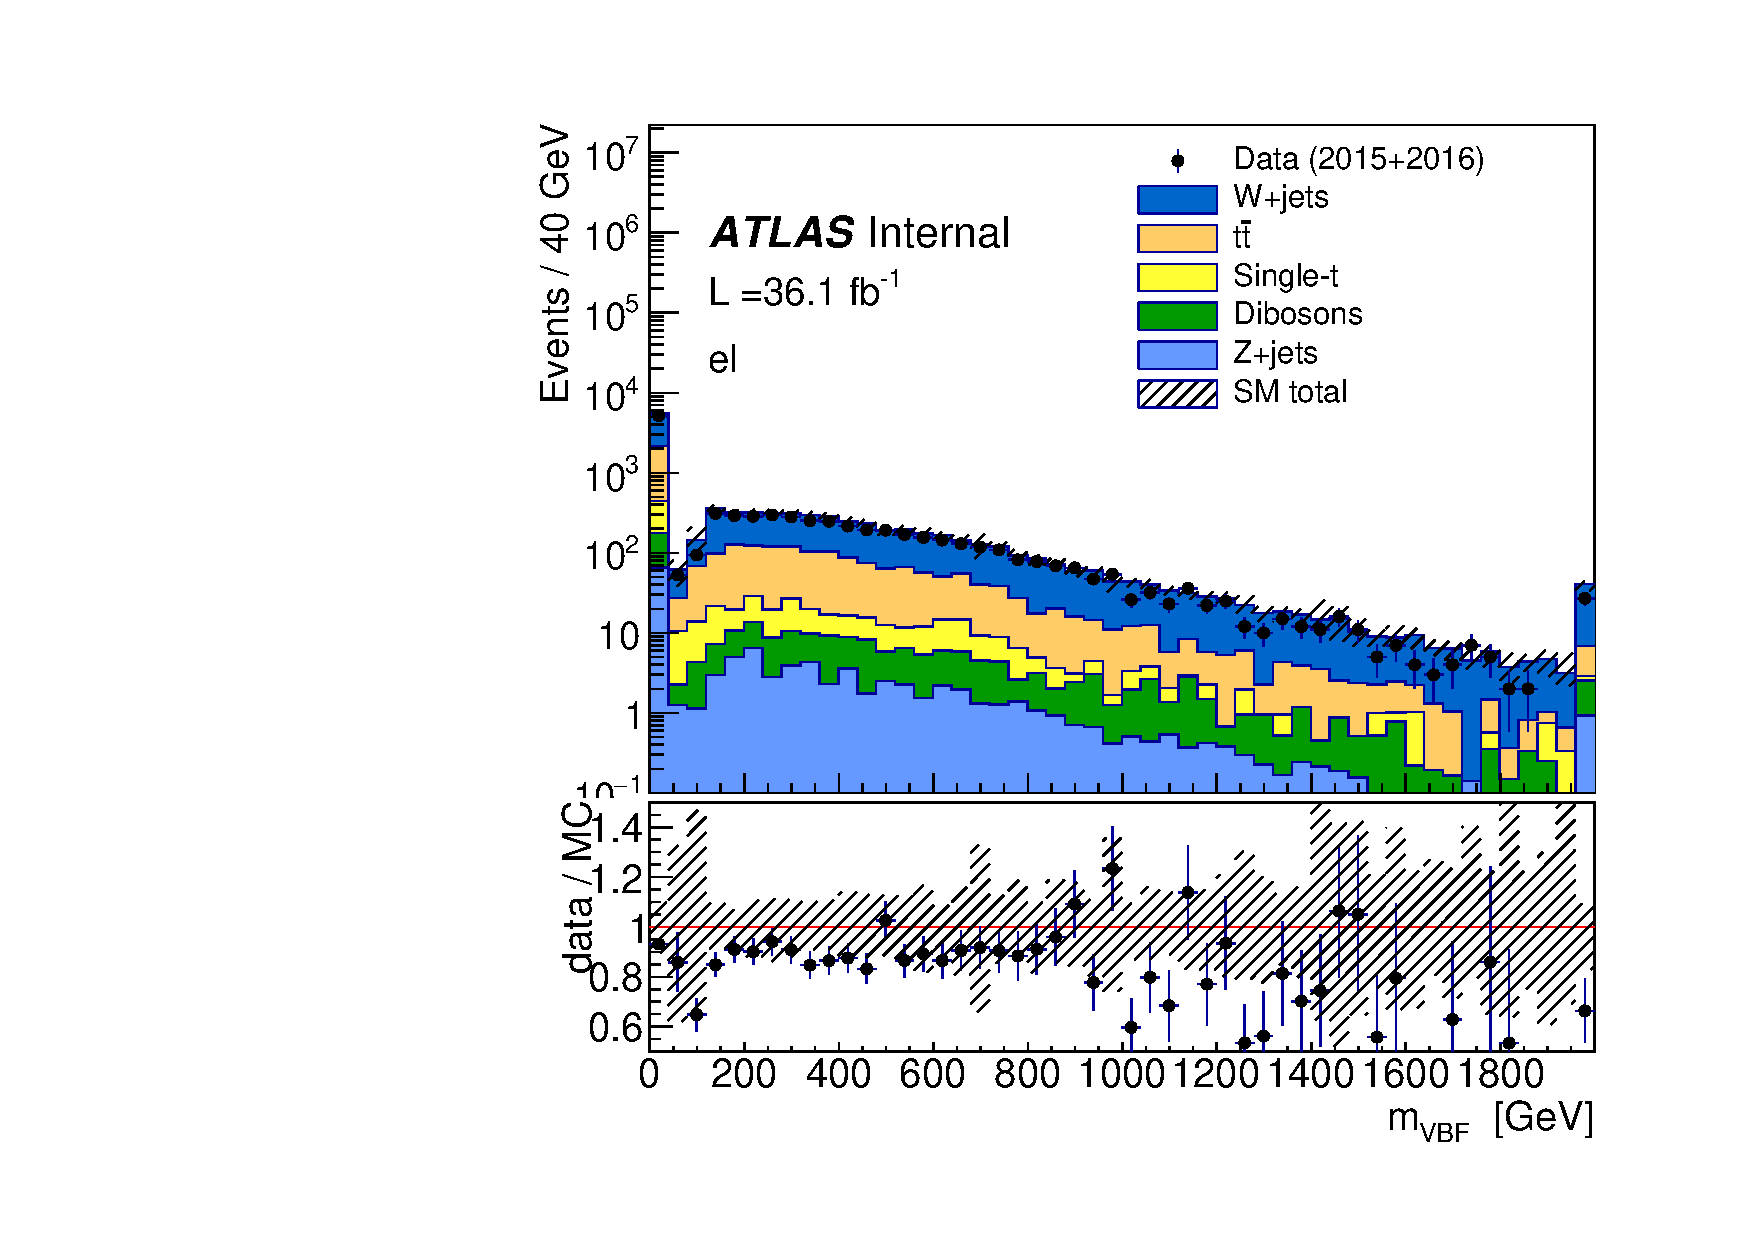
\includegraphics[width=0.43\textwidth]{Chapter3/VBF36fbHP/VBFmass_3_el}}
	\subfloat[]{\includegraphics[width=0.43\textwidth]{Chapter3/VBF36fbHP/VBFmass_3_mu}}\\
	\subfloat[]{\includegraphics[width=0.43\textwidth]{Chapter3/VBF36fbLP/VBFmass_12_el}}
    \subfloat[]{\includegraphics[width=0.43\textwidth]{Chapter3/VBF36fbLP/VBFmass_12_mu}}\\	
 	\subfloat[]{\includegraphics[width=0.43\textwidth]{Chapter3/ResolvedCR/VBF36fb/VBFmass_5_el}}
    \subfloat[]{\includegraphics[width=0.43\textwidth]{Chapter3/ResolvedCR/VBF36fb/VBFmass_5_mu}}\\   
	\caption{The distribution of $m_{jj}^{VBF}$ in VBF high purity (top), low purity (middle), and resolved (bottom) W+jet control region for electron (left) and muon (right) channels respectively}
	\label{Fig:mJJVBFWR}
\end{figure}


\begin{figure}[ht]
	\centering
	\subfloat[]{\includegraphics[width=0.43\textwidth]{Chapter3/VBF36fbHP/VVM_2_el}}
	\subfloat[]{\includegraphics[width=0.43\textwidth]{Chapter3/VBF36fbHP/VVM_2_mu}}\\
	\subfloat[]{\includegraphics[width=0.43\textwidth]{Chapter3/VBF36fbLP/VVM_13_el}}
    \subfloat[]{\includegraphics[width=0.43\textwidth]{Chapter3/VBF36fbLP/VVM_13_mu}}\\
	\subfloat[]{\includegraphics[width=0.43\textwidth]{Chapter3/ResolvedCR/VBF36fb/VVM_6_el}}
    \subfloat[]{\includegraphics[width=0.43\textwidth]{Chapter3/ResolvedCR/VBF36fb/VVM_6_mu.eps}}	
	\caption{The distribution of $m_{WV}$ in VBF high purity (top), low purity (middle), and resolved (bottom) top control region for electron (left) and muon (right) channels respectively}
	\label{Fig:mWVVBFTR}
\end{figure}
\clearpage
\begin{figure}[ht]
	\centering
	\subfloat[]{\includegraphics[width=0.43\textwidth]{Chapter3/VBF36fbHP/VBFmass_2_el}}
	\subfloat[]{\includegraphics[width=0.43\textwidth]{Chapter3/VBF36fbHP/VBFmass_2_mu}}\\
	\subfloat[]{\includegraphics[width=0.43\textwidth]{Chapter3/VBF36fbLP/VBFmass_13_el}}
    \subfloat[]{\includegraphics[width=0.43\textwidth]{Chapter3/VBF36fbLP/VBFmass_13_mu}}\\	
    \subfloat[]{\includegraphics[width=0.43\textwidth]{Chapter3/ResolvedCR/VBF36fb/VBFmass_6_el}}
    \subfloat[]{\includegraphics[width=0.43\textwidth]{Chapter3/ResolvedCR/VBF36fb/VBFmass_6_mu}}\\
	\caption{The distribution of $m_{jj}^{VBF}$ in VBF high purity (top), low purity (middle), and resolved (bottom) top control region for electron (left) and muon (right) channels respectivelyy}
	\label{Fig:mJJVBFTR}
\end{figure}

